\documentclass[whitelogo]{tudelft-report}
\usepackage{natbib}
%\bibliographystyle{abbrvnat}
\setcitestyle{authoryear,round,citesep={;},aysep={,},yysep={;}}
\usepackage{changes}
\usepackage{enumitem}
\usepackage{listings}
\usepackage{longtable}
\usepackage{amssymb}
\usepackage{pifont}
\usepackage[titletoc]{appendix}
\newcommand{\cmark}{\ding{51}}%
\newcommand{\xmark}{\ding{55}}%
\lstset{language=python, breaklines=true}
\setlist{nolistsep}

\renewcommand*{\sectionautorefname}{Section} % Rename the section hyperlink
\renewcommand*{\chapterautorefname}{Chapter} % Rename the section hyperlink

\begin{document}


%% Use Roman numerals for the page numbers of the title pages and table of
%% contents.
\frontmatter

% Uncomment following 19 lines for a cover with a picture on the lower half only
\title[tudelft-white]{Policy \\Emergence}
\subtitle[tudelft-cyan]{An agent-based approach - C\&F Update}
\author[tudelft-white]{R.\ Klein}
\affiliation{Technische Universiteit Delft}
\coverimage{newcover-01.png}
%\titleoffsetx{10cm}
%\titleoffsety{10cm}
\titleoffsetx{2cm}
\titleoffsety{23cm}
\afiloffsetx{1cm}
\afiloffsety{18cm}
\covertext[tudelft-white]{
    \textbf{Cover Text} \\
    possibly \\
    spanning 
    multiple 
    lines
    \vfill
    ISBN 000-00-0000-000-0
}
\makecover

%% Uncomment following 16 lines for a cover with a picture on the lower half only
%\title[tudelft-white]{Emergence of \\Policies}
%\subtitle[tudelft-black]{An agent-based \\approach}
%\author[tudelft-white]{R.\ Klein}
%\affiliation{Technische Universiteit Delft}
%%\coverimage{tank.jpg}
%\covertext[tudelft-white]{
%   % \textbf{Cover Text} \\
%   % possibly \\
%   % spanning 
%   % multiple 
%  %  lines
%   % \vfill
%    %ISBN 000-00-0000-000-0
%}
%\setpagecolor{tudelft-orange}
%\makecover[split]

\renewcommand*{\sectionautorefname}{Section} % Rename the section hyperlink
\renewcommand*{\chapterautorefname}{Chapter} % Rename the section hyperlink

%% Include an optional title page.
\begin{titlepage}


\begin{center}

%% Insert the TU Delft logo at the bottom of the page.

%% Print the title in cyan.
{\makeatletter
\largetitlestyle\fontsize{64}{94}\selectfont\@title
%\largetitlestyle\color{tudelft-cyan}\Huge\@title
\makeatother}

%% Print the optional subtitle in black.
{\makeatletter
\if\@subtitle\undefined\else
    \bigskip
   {\tudsffamily\fontsize{22}{32}\selectfont\@subtitle}    
    %\titlefont\titleshape\LARGE\@subtitle
\fi
\makeatother}

\bigskip
\bigskip

by
%door

\bigskip
\bigskip

%% Print the name of the author.
{\makeatletter
%\largetitlefont\Large\bfseries\@author
\largetitlestyle\fontsize{26}{26}\selectfont\@author
\makeatother}

\bigskip
\bigskip

to obtain the degree of Master of Science
%ter verkrijging van de graad van Master of Science

at the Delft University of Technology,
%aan de Technische Universiteit Delft,

to be defended publicly on Tuesday May 23, 2017 at 14:30 PM.
%in het openbaar de verdedigen op dinsdag 1 januari om 10:00 uur.

\vfill

\begin{tabular}{lll}
    Student number: & XXXXXXX \\
    Project duration: & \multicolumn{2}{l}{October 6, 2016 -- May 23, 2017} \\
    Thesis committee: & Dr.\ ir.\ I.\ Nikolic, & TU Delft, supervisor \\
    	& Prof.\ dr.\ ir.\ P.\ Herder, & TU Delft, chairwoman \\
        & Dr.\ P.\ Bots, & TU Delft
\end{tabular}
%% Only include the following lines if confidentiality is applicable.

\bigskip
\bigskip
%\emph{This thesis is confidential and cannot be made public until December 31, 2013.}
%\emph{Op dit verslag is geheimhouding van toepassing tot en met 31 december 2013.}

\bigskip
\bigskip
An electronic version of this thesis is available at \url{http://repository.tudelft.nl/}.
%\\[1cm]

%\centering{
\includegraphics{cover/logo_black}}


\end{center}

\begin{tikzpicture}[remember picture, overlay]
    \node at (current page.south)[anchor=south,inner sep=0pt]{
        
\includegraphics{cover/logo_black}
    };
\end{tikzpicture}

\end{titlepage}



\setcounter{tocdepth}{1}
\tableofcontents

%% Use Arabic numerals for the page numbers of the chapters.
\mainmatter

\renewcommand*{\sectionautorefname}{Section} % Rename the section hyperlink
\renewcommand*{\chapterautorefname}{Chapter} % Rename the section hyperlink

% This corresponds to the file with the old explanations on the template of this report.
%\chapter{Introduction}

%\cite{zahariadis2014ambiguity, zahariadis2007multiple, witting2012role}

This document is intended to be both an example of the TU Delft \LaTeX{} template for reports and theses, as well as a short introduction to its use. It is not intended to be a general introduction to \LaTeX{} itself,\footnote{We recommend \url{http://en.wikibooks.org/wiki/LaTeX} as a reference and a starting point for new users.} and we will assume the reader to be familiar with the basics of creating and compiling documents.

Instructions on how to use this template under Windows and Linux, and which \LaTeX{} packages are required, can be found in \texttt{README.txt}.

\section{Document Structure}

Since a report, and especially a thesis, might be a substantial document, it is convenient to break it up into smaller pieces. In this template we therefore give every chapter its own file. The chapters (and appendices) are gathered together in \texttt{report.tex}, which is the master file describing the overall structure of the document. \texttt{report.tex} starts with the line
\begin{quote}
    \texttt{\textbackslash documentclass\{tudelft-report\}}
\end{quote}
which loads the TU Delft report template. The template is based on the \LaTeX{} \texttt{book} document class and stored in \texttt{tudelft-report.cls}. The document class accepts several comma-separated options. The default language is English, but this can be changed to Dutch (\emph{e.g.}, for bachelor theses) by specifying the \texttt{dutch} option:
\begin{quote}
    \texttt{\textbackslash documentclass[dutch]\{tudelft-report\}}
\end{quote}
Furthermore, hyperlinks are shown in blue, which is convenient when reader the report on a computer, but can be expensive when printing. They can be turned black with the \texttt{print} option. This will also turn the headers black instead of cyan.

If the document becomes large, it is easy to miss warnings about the layout in the \LaTeX{} output. In order to locate problem areas, add the \texttt{draft} option to the \texttt{\textbackslash documentclass} line. This will display a vertical bar in the margins next to the paragraphs that require attention. Finally, the \texttt{nativefonts} option can be used to override the automatic font selection (see below).

This template has the option to automatically generate a cover page with the \texttt{\textbackslash makecover} command. See the next section for a detailed description.

The contents of the report are included between the \texttt{\textbackslash begin\{document\}} and \texttt{\textbackslash end\{document\}} commands, and split into three parts by
\begin{enumerate}
\item\texttt{\textbackslash frontmatter}, which uses Roman numerals for the page numbers and is used for the title page and the table of contents;
\item\texttt{\textbackslash mainmatter}, which uses Arabic numerals for the page numbers and is the style for the chapters;
\item\texttt{\textbackslash appendix}, which uses letters for the chapter numbers, starting with `A'.
\end{enumerate}
The title page is defined in a separate file, \emph{e.g.}, \texttt{title.tex}, and included verbatim with \texttt{\textbackslash input\{title\}}.\footnote{Note that it is not necessary to specify the file extension.} Additionally, it is possible to include a preface, containing, for example, the acknowledgements. An example can be found in \texttt{preface.tex}. The table of contents is generated automatically with the \texttt{\textbackslash tableofcontents} command. Chapters are included after \texttt{\textbackslash mainmatter} and appendices after \texttt{\textbackslash appendix}. For example, \texttt{\textbackslash input\{chapter-1\}} includes \texttt{chapter-1.tex}, which contains this introduction.

The bibliography, finally, is generated automatically with
\begin{quote}
    \texttt{\textbackslash bibliography\{report\}}
\end{quote}
from \texttt{report.bib}. The bibliography style is specified in \texttt{tudelft-report.bst}, which is a modified version of \texttt{apsrev4-1.bst} (from REVTeX) designed to also display the titles of referenced articles. The template will automatically generate clickable hyperlinks if a URL or DOI (digital object identifier) is present for the reference. As an example, we cite the paper by Nobel laureate Andrei Geim and his pet hamster \citep{Geim2001}. Although it is possible to manage the bibliography by hand, we recommend using EndNote (available from Blackboard) or JabRef (available from \url{http://jabref.sourceforge.net/}).

\section{Cover and Title Page}

This template will automatically generate a cover page if you issue the \texttt{\textbackslash makecover} command. There are two formats for the cover page: one with a page-filling (`bleeding')
illustration, with the title(s) and author(s) in large ultrathin typeface, and the other where the illustration fills the lower half of the A4, whereas title(s), author(s) and additional
text are set in the standard sans-serif font on a plain background with a color chosen by the user. The last option is selected by the optional key \texttt{split}: \texttt{\textbackslash makecover[split]} yields
a page with the illustration on the lower half. All illustrations are bleeding, in accordance with the TU Delft style.

Before generating the cover, you need to provide the information to put on it. This can be done with the following commands:
\begin{itemize}
\item\texttt{\textbackslash title[Optional Color]\{Title\}} \\
    This command is used to provide the title of the document. The title
    title is also printed on the spine. If you use a title page (see below), this information will be used there as well.
    As the title, subtitle and author name are printed directly over the cover photo, it will often be necessary to adjust the print color in order to have
    sufficient contrast between the text and the background. The optional color argument is used for this.
\item\texttt{\textbackslash title[Optional Color]\{Subtitle\}} \\
    This command is used to provide a subtitle for the document. If you use a title page (see below), this information will be used there as well.
    It possible to adjust the print color in order to have
    sufficient contrast between the text and the background -- the optional color argument is used for this.
\item\texttt{\textbackslash author\{J.\ Random Author\}} \\
    This command specifies the author. The default color is \texttt{tudelft-white}, but this may be adjusted in the same way as the titles.
\item\texttt{\textbackslash affiliation\{Technische Universiteit Delft\}} \\
    The affiliation is the text printed vertically on the front cover. It can be the affiliation, such as the university or department name, or be used for the document type (\emph{e.g.}, Master's thesis). The default color is again \texttt{tudelft-white}, adjustable through the \texttt{color} option.
\item\texttt{\textbackslash coverimage\{cover.jpg\}} \\
    With this command you can specify the filename of the cover image. The image is stretched to fill the full width of the front cover (including the spine if a back cover is present).
\item\texttt{\textbackslash covertext\{Cover Text\}} \\
    If a back cover is present, the cover text is printed on the back. Internally, this text box is created using the \LaTeX{} \texttt{minipage} environment, so it supports line breaks.
\item\texttt{\textbackslash titleoffsetx\{OffsetX\},\textbackslash titleoffsety\{OffsetY\}}
    If the cover page contains a page-filling picture (i.e., \texttt{split} is not specified with the \texttt{makecover} command, the best position of the title depends a lot on the picture chosen for it. The lower left corner of the minipage containing title, subtitle and author is 
    specified by these two commands. The offsets are measured from the top left corner of the page. 
\item\texttt{\textbackslash afiloffsetx\{AfilX\}, \textbackslash afiloffsety\{AfilY\}}
    specifies the lower left corner of the text containing the affiliation, measured from the top left corner of the page. 
\end{itemize}

In addition to \texttt{[split]}, the \texttt{\textbackslash makecover} command accepts several additional options for customizing the layout of the cover. 
The most important of these is \texttt{back}. Supplying this option will generate a back cover as well as a front, including the spine. Since this requires a page size slightly larger than twice A4 (to make room for the spine), and \LaTeX{} does not support different page sizes within the same document, it is wise to create a separate file for the cover. \texttt{cover.tex} contains an example. The recommended page size for the full cover can be set with
\begin{quote}
    \textbackslash geometry\{papersize=\{1226bp,851bp\}\}
\end{quote}
after the document class and before \texttt{\textbackslash begin\{document\}}.

The other options \texttt{\textbackslash makecover} accepts are
\begin{itemize}
\item\texttt{nospine} \\
    If a back cover is generated, the title will also be printed in a black box on the spine. However, for smaller documents the spine might not be wide enough. Specifying this option disables printing the title on the spine.
\item\texttt{frontbottom} \\
    By default the black box on the front is situated above the blue box. Specifying this option will place the black box below the blue one.
\item\texttt{spinewidth} \\
    If a back cover is present, this option can be used to set the width of the spine. The default is \texttt{spinewidth=1cm}.
\item\texttt{frontboxwidth}, \texttt{frontboxheight}, \texttt{backboxwidth}, \texttt{backboxheight} \\
    As their names suggest, these options are used to set the width and height of the front (black) and back (blue) boxes. The default widths and heights are \texttt{4.375in} and \texttt{2.1875in}, respectively.
\item\texttt{x}, \texttt{y} \\
    The blue and black boxes touch each other in a corner. The location of this corner can be set with these options. It is defined with respect to the top left corner of the front cover. The default values are \texttt{x=0.8125in} and \texttt{y=3in}.
\item\texttt{margin} \\
    This option sets the margin between the borders of the boxes and their text. The default value is \texttt{12pt}.
\end{itemize}

For a thesis it is desirable to have a title page within the document, containing information like the thesis committee members. To give you greater flexibility over the layout of this page, it is not generated by a command like \texttt{\textbackslash makecover}, but instead described in the file \texttt{title.tex}. Modify this file according to your needs. The example text is in English, but Dutch translations are provided in the comments. Note that for a thesis, the title page is subject to requirements which differ by faculty. Make sure to check these requirements before printing.

\section{Chapters}

Each chapter has its own file. For example, the \LaTeX{} source of this chapter can be found in \texttt{chapter-1.tex}. A chapter starts with the command
\begin{quote}
    \texttt{\textbackslash chapter\{Chapter title\}}
\end{quote}
This starts a new page, prints the chapter number and title and adds a link in the table of contents. If the title is very long, it may be desirable to use a shorter version in the page headers and the table of contents. This can be achieved by specifying the short title in brackets:
\begin{quote}
    \texttt{\textbackslash chapter[Short title]\{Very long title with many words which could not possibly fit on one line\}}
\end{quote}
Unnumbered chapters, such as the preface, can be created with \texttt{\textbackslash chapter*\{Chapter title\}}. Such a chapter will not show up in the table of contents or in the page header. To create a table of contents entry anyway, add
\begin{quote}
    \texttt{\textbackslash addcontentsline\{toc\}\{chapter\}\{Chapter title\}}
\end{quote}
after the \texttt{\textbackslash chapter} command. To print the chapter title in the page header, add
\begin{quote}
    \texttt{\textbackslash setheader\{Chapter title\}}
\end{quote}

Chapters are subdivided into sections, subsections, subsubsections, and, optionally, paragraphs and subparagraphs. All can have a title, but only sections and subsections are numbered. As with chapters, the numbering can be turned off by using \texttt{\textbackslash section*\{\ldots\}} instead of \texttt{\textbackslash section\{\ldots\}}, and similarly for the subsection.
\section{\textbackslash section\{\ldots\}}
\subsection{\textbackslash subsection\{\ldots\}}
\subsubsection{\textbackslash subsubsection\{\ldots\}}
\paragraph{\textbackslash paragraph\{\ldots\}}
Lorem ipsum dolor sit amet, consectetur adipisicing elit, sed do eiusmod tempor incididunt ut labore et dolore magna aliqua. Ut enim ad minim veniam, quis nostrud exercitation ullamco laboris nisi ut aliquip ex ea commodo consequat. Duis aute irure dolor in reprehenderit in voluptate velit esse cillum dolore eu fugiat nulla pariatur. Excepteur sint occaecat cupidatat non proident, sunt in culpa qui officia deserunt mollit anim id est laborum.

\section{Fonts and Colors}

The fonts used by this template depend on which version of \LaTeX{} you use. Regular \LaTeX, \emph{i.e.}, if you compile your document with with \texttt{latex}, \texttt{pslatex} or \texttt{pdflatex}, will use Utopia for text, Fourier for math and Latin Modern for sans-serif and monospaced text. 
However, if you want to adhere to the TU Delft house style, you will need to use \XeLaTeX, as it supports TrueType and OpenType fonts. Compiling with \texttt{xelatex} will use Arial for most titles and text, Courier New for monospace and Cambria for math. If you want to haf a sans-serif font for the
main text, while using \texttt{latex}, \texttt{pslatex} or \texttt{pdflatex}, you can use the option \texttt{noroman} in the report style: \texttt{\textbackslash usepackage[\ldots,noroman]{tudelft-report}}. For document and part titles,  TU Delft Ultra Light is used. For quotes, columns and text in boxes, you use Georgia. If you want to use \XeLaTeX, but do not want to use the TU Delft house style fonts, you can add the \texttt{nativefonts} option to the document class. This will still use  TU Delft Utra Light and Arial on the cover, but not for the body of the document. If you need to use these fonts for certain sections in the main text, they are available via \texttt{\textbackslash tudrmfamily} (Georgia) and \texttt{\textbackslash tudtitlefamily} (TU Delft Utra Light).

\begin{quote}
  You have to learn the rules of the game. And then you have to play better than anyone else.\\
  \emph{Albert Einstein}
\end{quote}

The corporate colors of the TU Delft are cyan, black and white, available via \texttt{\textbackslash color\{{\color{tudelft-cyan}tudelft-cyan}\}}, \texttt{\textbackslash color\{{\color{tudelft-black}tudelft-black}\}} (which differs slightly from the default \texttt{\textbackslash color\{black\}}) and \texttt{\textbackslash color\{tudelft-white\}}, respectively. Apart from these three, the house style defines the basic colors \texttt{\color{tudelft-sea-green}tudelft-sea-green}, \texttt{\color{tudelft-green}tudelft-green}, \texttt{\color{tudelft-dark-blue}tudelft-dark-blue}, \texttt{\color{tudelft-purple}tudelft-purple}, \texttt{\color{tudelft-turquoise}tudelft-turquoise} and \texttt{\color{tudelft-sky-blue}tudelft-sky-blue}, as well as the accent colors \texttt{\color{tudelft-lavendel}tudelft-lavendel}, \texttt{\color{tudelft-orange}tudelft-orange}, \texttt{\color{tudelft-warm-purple}tudelft-warm-purple}, \texttt{\color{tudelft-fuchsia}tudelft-fuchsia}, \texttt{\color{tudelft-bright-green}tudelft-bright-green} and \texttt{\color{tudelft-yellow}tudelft-yellow}.



%====== Revised conceptualisation
\chapter{The Conceptualisation}
\label{cha:conceptualisationRevised}
This chapter presents the entire revised conceptualisation. It was revised after reflection on the actions. The formalisation is similarly revised in the next appendix.

\section{Common core}
\label{sec:conceptualisationCommonCoreRevised}

The policy emergence process is a process composed of several {\bfseries iterative stages}. Different iterative stages can be differentiated. There are iterative stages where the {\bfseries actors} present in the {\bfseries policy arena} interact with each other. The policy arena is the environment in which these connected actors evolve. Additionally, different types of actors are present within the policy arena. They are the {\bfseries policy makers}, the {\bfseries policy entrepreneurs} and the {\bfseries external parties}. The policy makers are the actors that have decision making power. This means that they can decide what is placed on the {\bfseries agenda} or what {\bfseries policy instrument} should be implemented. The former is performed in the round called the {\bfseries agenda setting} while the latter is perform during the round called the {\bfseries policy formulation}. They can also work to influence the {\bfseries beliefs} of the other actors present in the policy arena which are connected to them through their {\bfseries policy network}. The policy network is the network that connects the actors present in one policy arena. The actors are connected based on their awareness of one another. The likelihood of actors to interact with one another is dependent on their awareness of one another. Over time the policy network of the actors will deteriorate. To maintain their network, the actors are able to perform simple actions using their {\bfseries resources}. These resources represent their financial and political resources.

Each policy maker possesses a belief hierarchy that defines its beliefs on the issues being discussed in the policy arena. This hierarchy is composed of field wide beliefs at the top and beliefs on increasingly detailed issues when progressing downwards in the hierarchy. Example of issues are public transportation or the amount of plastic present with a size less than 2 millimetres present in the oceans. For each of these issues, the actors have an understanding of the current {\bfseries states of the world} and a goal for where they would like to see this issue be. Furthermore, each level in the hierarchy is connected to the next through causal relations up to the highest level. These causal relations help the actor understand how different issues affect each other and therefore how the world works.

The impact of the influence of the policy makers on the other actors is dependent on the resources spent by the policy makers, the difference in beliefs they have with the actor they are influencing and the affiliation of both influencing and influenced actor. However, before influencing other actors, a decision must be made on what influence should be performed and on which actor. The likelihood that a policy maker will influence another actor will vary depending on their {\bfseries political affiliation} in relation to the affiliation of the actor influenced, their perceived {\bfseries conflict level} on the issues concerned with the actor influenced, their policy network (awareness level) and whether the actor being influenced is a policy maker or another actor. Within the policy arena, actors will prefer influencing policy makers as they have decision making power (they decide on the agenda and the policy instrument to be implemented). The political affiliation of the actors relates them to specific {\bfseries constituencies}. Furthermore, it affects the likelihood of actors of different affiliation of interacting with one another. The resources available to the policy makers are dependent on the size of their affiliated constituencies. There is a conflict level for each issue represented in the beliefs of a policy maker. This conflict level is the difference in the views of the world of the policy maker and what the policy maker thinks the beliefs of the actors influenced are. This perception of actor B’s beliefs by actor A is referred to as the {\bfseries partial knowledge} of the actor A. The amount of conflict level will affect the likelihood of the two actors interacting with one another about certain issues. Actors are more likely to discuss issues for which they have a mild conflict level and less likely to discuss issues for which they have a high conflict level.

There are different types of actions which the policy makers can perform on the other actors. They can perform {\bfseries framing actions}. These actions are attempts to influence other actors on their beliefs of how the world works (the causal relations in their beliefs hierarchies). The policy makers can also {\bfseries directly influence} the actors on their beliefs for the issues. They can influence them on the way they see the world or on their aims of what the world should be. Because the {\bfseries attention span} of the actors in the policy arena is limited, these actors tend to only influence other actors on one selected issue. This issue is selected based on the appearance of {\bfseries urgency}. This urgency is determined by the actors based on the gap between the current states of the world and their aim but also in relation to the impact that this issue ultimately has on their normative beliefs. The ultimate goals of the policy makers being to reach their normative belief goals. 

The partial knowledge of the actors is updated whenever an influencing action is performed. Both the actor influencing and the actor being influenced have been part of the interaction and therefore get a better, but not perfect, understanding of each other’s beliefs on the topic of the interaction.

As mentioned earlier, the policy makers can also decide what is on the agenda. This is done by selecting the issue that they consider to be the most urgent to them. The issue that is ultimately placed on the agenda is the issue that most policy makers believe is urgent. The choice of issue on the agenda will go on to define which issues can be discussed in iterative stages looking at lower level issues in the belief hierarchies. The issues all have to be related to the issue on the agenda. This is however subjective to the actors depending on their personal beliefs. The process of agenda setting therefore helps narrow down the problems observed by the policy makers and to ultimately decide on a {\bfseries policy instrument} that can be used to address such problem.

The policy entrepreneurs are actors that seek to influence the beliefs of the policy makers primarily but also to influence the beliefs of the other actors within the policy arena through their policy network. Their aim is to push their beliefs onto the other actors present in the arena. Similarly to the policy makers, the policy entrepreneurs have a belief hierarchy, a political affiliation and use resources to influence other actors. These resources are also defined based on their constituencies. They can also perform different actions on the policy makers, external parties and other policy entrepreneurs. They can frame how the world works, influence on the beliefs of other actor’s view of the world and their goals. The likelihood of performing an action and its actual impact are determined in a similar way as for the policy makers.

The external parties are actors that have multiple roles within the policy arena. The external parties represent actors such as the media, but also research institute or academic institutions. They help inform other external parties, the policy makers, the policy entrepreneurs about the current state of the world. They can also influence other external parties, policy makers and policy entrepreneurs on their beliefs of how the world works, on issue states and on issue aims. Finally, they can influence the goals of the constituencies. Similarly to the policy makers, the external parties have a certain political affiliation and resources stemming from that affiliation.

The external parties have direct access to the states of the world. They can therefore transmit this information to the actors within the policy arena along with the constituencies. However, not all external parties are interested in all states of the world, some external parties are only interested in specific states. Furthermore, this transmission of the states is dependent on the policy network, and the affiliation of the external parties and the actors to whom they are transmitting this information. Different actors will perceive the external parties as more or less trust worthy depending on their affiliation.

The external parties can also influence other external parties, the policy makers and the policy entrepreneurs. They can do this through framing actions, influence on aim actions and influence on state actions that affect all actors present in the policy arena called blanket actions. The likelihood of performing a blanket action is defined the same way as for the policy makers. The impact is  obtained as shown earlier on. The impact is however spread on all actors concerned. 

Finally, the external parties can influence the goals of the different constituencies through blanket influence. This is similar to the blanket framing that is used on the actors within the policy arena but this time they affect the others' goals. The likelihood of an action being performed will depend on the difference in beliefs between the constituencies and the external party concerned and the affiliation of the external party performing this action. The impact will depend on the resources spent and the difference in beliefs.

Each constituency represent a sector of the electorate and is associated to a political affiliation. Each constituency represents a certain percentage of the total voter population. This representativeness of a constituency is what affects the amount of resources that is distributed to the different actors within the policy arena as mentioned previously. The constituencies can influence the policy makers present in the policy arena. The policy maker’s goal beliefs tend to move towards the goals of their constituencies to increase their chance of remaining in office.

A second round can also be identified as a policy formulation round. In this round, the aim is to adopt a policy instrument based on the chosen agenda such that it is implemented in the world. Policy instruments are the specific mechanisms policy makers put in place in order to impact the issues discussed within the iterative stages. During the policy formulation round, the actors influence each other’s beliefs similarly to the agenda setting round. The aim here is however different. Each actor selects a policy instrument based on its expected impact in the world. This impact is assessed by the actors based on their beliefs of the change the instrument will have on the states of each issues compared to their own goals. Because the actors have a limited attention span, they can only select what they perceive as being the most appropriate policy instrument. They decide that based on the impact that the instrument have on their beliefs and based on which issues need to be addressed the most urgently. The interactions of the different actors are the same as for the agenda setting round. The likelihood of an action happening is however now determined based on the expected impact that each instrument has on the urgent issues in the actors’ beliefs within the narrower field of issues selected in the agenda setting stage.

One main difference is that the policy formulation round does not end with the selection of an issue but the selection of a policy instrument. Furthermore, the policy instrument selected is only implemented if the number of policy makers that support that instrument is superior to the threshold required for the implementation of the instrument. This threshold can be a majority, a two third majority or unanimity.

The last round considered is a round that does not involve the actors. It is the world. In this round, the instrument that has been selected is implemented. The world is affected by that instrument and the states of the world change accordingly. This then has an impact on the belief of the actors present in the policy arena as the change in the states is conveyed by the external parties to the different actors.

Finally external events can be introduced in the model. Such external events can affect anything from the goal of specific agents for a specific issue to a new distribution of the constituencies. These external events are devised based on case studies. The modeller must then adopt the impact of an election into the model’s framework to appropriately represent that election.

\section{Three streams theory}
\label{sec:conceptualisation3SRevised}

The introduction of the three streams theory changes some of the aspects presented in the common core. These changes are performed to account for the concept of streams and of policy window. The iterative stages considered are the same as the iterative stages mentioned in the common core. The difference is present in what the actors present in the policy arena choose as an issue. The actors can now choose from a policy or a problem as called for in the three streams theory. The problems are obtained in the belief hierarchy of the actors while the policy are obtained in a {\bfseries policy hierarchy}. 

The policy hierarchy is a hierarchy containing policy instruments. These policy instruments have specific impacts on the issues present in the belief hierarchy of the actors. The concept of policy instrument is therefore the same as the one presented in the common core. Within the three streams theory, policy instruments are present in all iterative stages. Each of these impact is now subjective which means that they also represent beliefs on the effectiveness of the different policies. These beliefs can also be influenced by the different actors present in the policy arena.

Each actor first selects a policy or a problem. The problems are graded similarly to what was previously presented in the common core: based on the perceived urgency of the chosen issue. The policy are graded based on their impact on their associated issues. Whichever grade is the highest will be chosen by the actor. If the actor chooses a problem first, then s/he will have to choose an associated policy based on the effectiveness of the policies. Furthermore, all actions performed by that actor from now on will be on the beliefs of other actors concerning the selected problem. These actions re the same as the ones in the common core. If an actor chooses a policy first, s/he will have to choose an associated problem based on urgency. Similarly to the problem, all actions performed by that actor from now on will be on the beliefs of other actors concerning the selected policy.

The policy actions are similar to the problem actions presented in the common core for the different actors but with one change to the framing action. The aim of the actor is now to affect the impact beliefs of other actors in their policy network. The actions on policies are therefore akin to the framing actions related to the problems. This can only be done by actors having first selected a policy as mentioned earlier. There are some important caveats to this approach. First, the constituencies do not possess any beliefs on the policy hierarchy. This means that external parties cannot influence the constituencies if they have selected a policy first, they will then move on to their problem (which they selected based on the policy first chosen) and influence the constituencies on that problem. Second, the constituencies cannot influence the instrument hierarchy of the policy makers, the influence remains focused only on the belief hierarchy.

Additionally to the introduction of streams, the policy entrepreneurship model which is tied to the three streams theory introduces the concept of {\bfseries teams}. Teams are small, short-term groups of actors which try to influence other actors on a specific problem or policy. These teams are constituted by actors when they consider that a policy or a problem is very urgent and when they can find other actors that share their beliefs on that policy or problem and the urgency of it. Once a problem or policy has been sufficiently pushed (enough actors have been influenced), then the team will disband and the actor will return to acting separately. Teams use the same actions as the individual actors. They provide actors with a larger policy network. This is because the team network consists of the sum of the networks of all actors present in the team. The teams obtain their resources from their members based on their feeling of belonging within a team. The actions performed by the team have to be agreed by the entire team as team are non-centralised entities. This means that no actor is powerful enough to impose his/her will on the other actors. Teams can also perform influencing actions on their own members. This helps increase the cohesiveness of the team so that they can last longer within the policy arena. The actions performed by team members on team members are blanket framing, influence on goals an influence on states.

Although there are also a set of iterative stages in the three streams theory, the actions performed in both iterative stages are not different anymore. Because each actor must have chosen either a policy or a problem, the actions are exactly the same in both iterative stages for all actors present in the policy network. The difference remains in the fact that for the agenda setting iterative stages, an agenda is set at the end which defines what is discussed thereafter. The agenda is composed of a problem and a policy. Each is chosen as being the most selected by the policy makers. The problems and policies discussed thereafter must relate to the problem and policy on the agenda. They must therefore be on a lower level in their respective hierarchies. For the policy formulation, the policy instrument chosen by the policy maker is the one that meets the threshold requirement once again. This disregard the fact that a policy maker might have chosen a problem first.

\section{The advocacy framework coalition}
\label{sec:conceptualisationACFRevised}

The introduction of the advocacy coalition framework adds some different changes to the common core. The main addition is the concept of {\bfseries coalitions}. The coalitions are groups to which actors are assigned based on their normative beliefs. They are long term entities that perform actions on other actors or other coalitions to influence them into similar beliefs. Actors only change coalitions when their normative beliefs vary which happens only rarely. The actions performed by coalitions are similar to the ones performed by teams. However, coalitions are centralised entities. This means that the {\bfseries coalition} leader is the only actor that decides which actions are implemented. The coalition leader is the actor within a coalition that has the largest policy network. Finally, the number of coalitions present within a policy arena is usually limited to only a few according to the literature. 

The ACF also introduces the policy broker. Policy brokers are actors that look in their network to put in contact actors which are badly connected within the policy arena. Policy makers, policy entrepreneurs and external parties can all be elevated to the role of policy broker which grants them additional actions. Two actions are added. With the first action, the policy broker can connect two actors which are not connected (but to which s/he is connected). In the second action, the policy broker can raise the awareness level between two actors (if his/her own awareness level is high enough). To perform these actions, the policy brokers is provided with additional resources fitting with the strength of his/her policy network.

Finally, which action is chosen by the policy broker is decided based on the type of policy broker. Neutral policy brokers will select the actions that will lead to the largest impact. This means that connecting actors that are not yet connected will come first, followed by raising the awareness between actors that are already aware of each other. If the policy broker plays an advocacy role, then s/he will select actions with actors that share his beliefs.

\section{Feedback theory}
\label{sec:conceptualisationFeedbackRevised}

For the feedback theory, the policy instruments implemented by the actors are supplemented with feedback effects. The feedback effects have an additional specified effect on different parts of the world or of the policy arena. When choosing for a policy instruments, the actors are not aware of the feedback effects. There are three feedback effects considered.

Some feedback effects have an impact on the constitution of the constituencies. The percentage distribution of each constituency will be affected. Some feedback effects have an impact on the belief hierarchy of the actors opening new issues to consideration in the hierarchy or removing others. Finally, a third feedback effect relates to the link between constituencies and the resources of the actors within the model. This links is affected by this type of feedback effects.

\section{Diffusion theory}
\label{sec:conceptualisationDiffusionRevised}

The introduction of the diffusion theory requires the consideration of multiple policy subsystems. These subsystems can represent different nations or cities for example but they are all regarding the same issues. The diffusion theory specifies the impact that the actors in a subsystem might have on actors of another subsystem. The subsystems share specific relationships ranging from {\bfseries friendly} to {\bfseries competitive} while considering {\bfseries coercive} and {\bfseries dominant}. These relationships help define the actions that can be considered between the actors of the different subsystems. Each subsystem also possesses a certain {\bfseries status}. This status helps define the amount of resources that is provided to each of their actors.

The actors in the different subsystems are all part of a {\bfseries super-policy network}. This network connects actors between the different subsystems. Through this network actors can influence each other depending on the relationships between the arenas. An actor will consider all possible actions. The actions that is most likely to be performed is implemented.

The subsystems themselves are part of a network. Each subsystem has a link with another. Each of these links are one directional and can be of one type from friendly to competitive. Links that are coercive or dominant also gain a {\bfseries strength} attribute. This strength attribute defines the influence that a subsystem will have on another when actors from one arena influence actors in the other. The actions that actors can perform is defined by the link that links their respective subsystems.

In the case of friendly relationship, the actor will be able to perform all actions that are available within the common core. These are actions of framing, influence on states and goals for the beliefs of the other actor. The likelihood of performing these actions along with their impact is assessed the same way as presented previously. When considering the diffusion theory with the common core or the ACF, then the actions are only performed on the issues. When it is considered with the three streams theory, then problems and policies actions are possible.

In the case of a coercive or dominant relationship, the actors will force their own goal beliefs onto selected actors in the other subsystem. The likelihood of this forced influence to be selected will depend on the conflict level between the actors and the type of actors that is being influenced (policy makers are more likely to be influence). Considering actions with an equal impact, actions on a dominant relationship will be most likely to happen, followed by coercive actions and finally friendly actions. The actual impact will only include the amount of resources spent, the difference in beliefs between the two actors and the strength of the considered subsystems. Once again, for similar actions, the impact will be largest in a dominant relationship.

In the case of a competitive relationship, the actors within one subsystem will seek to get a better world that the ones in other subsystems. To achieve this, they will change their goals to match the ones of other subsystems. This is also done through interactions. The likelihood of performing such an action along with their impact will is calculated similarly to the actions between friendly subsystems. The main difference with respect to the impact is that the impact of the actions are on the actor performing the action (the actor influences him/herself based on the beliefs of an actor in another subsystem).

%====== Revised formalisation
\chapter{The Formalisation}
\label{cha:formalisationRevised}
%Due to the iterative process and after a reflection period, several parts of the formalisation was modified. This was done after the code had been implemented, it is therefore not mentioned in the main body of this report. The changes considered are presented here.

Most of the changes considered are related to the way the actions are assessed by the actors and how their likelihood and impact are calculated. In the formalisation presented earlier on, the actions are graded based on their impact on the preferences of the agents being influenced. This is considered to be a stretch when considering real life actions. Instead, it was decided thereafter to use the likelihood of performing an action. This is determined by the agent based on conflict level, awareness of other agents or type of agents. The modified actions and equations are presented below.

Furthermore, as it was mentioned several times within the report, the actions of the external parties are harmonised with the other active actors. They can therefore perform four types of actions but all under a blanket form. The equations for these actions are also provided below.

%0
\paragraph{Individual framing}

The agents can attempt to influence the causal relation belief of other agents. This is an individual framing action. For this action, all causal relations related to the issue selected by the agent are considered. The likelihood to perform such an action depends on several parameters which are outlined below:

\begin{equation}\label{eq:likelihoodFraming2}
G_{CW, n_m} = conflictLevel_{CW, n, m} \cdot affiCoef_{Aff_n,Aff_m} \cdot awareness_{n,m} \cdot actionWeight_{n,m}
\end{equation}

where $G$ stands for the grade, $n$ is the influencing agent, $m$ is the influenced agent. $n_m$ is the perfection of the beliefs of the influenced agent by the influencing agent and $CW$ is the causal weight of the causal relation

If this action is selected, as it has the highest grade, then the impact of the action on the beliefs of the influenced agents is given by:

\begin{equation}\label{eq:impactFraming2}
CW_{m} := CW_{m} + \left(CW_{n} - CW_{m} \right) \cdot resources \cdot affiCoef_{Aff_n,Aff_m}
\end{equation}

%0
\paragraph{Individual action - Aim change}

The agents can also attempt to influence the aim beliefs on the different issues of the hierarchy of other agents. The likelihood that such action be performed is obtained in a similar way as shown below:

\begin{equation}\label{eq:likelihoodAimChange2}
G_{A, n_m} = conflictLevel_{A, n, m} \cdot affiCoef_{Aff_n,Aff_m} \cdot awareness_{n,m} \cdot actionWeight_{n,m}
\end{equation}

The impact of such action is then calculated with:

\begin{equation}\label{eq:impactAimChange2}
A_{m} := A_{m} + \left(A_{n} - A_{m} \right) \cdot resources \cdot affiCoef_{Aff_n,Aff_m}
\end{equation}

%0
\paragraph{Individual action - State change}

Similarly to the influence on the aims of an agent, the states can also be influenced. The likelihood of such an action being performed is given as follows:

\begin{equation}\label{eq:likelihoodStateChange2}
G_{S, n_m} = conflictLevel_{S, n,m} \cdot affiCoef_{Aff_n,Aff_m} \cdot awareness_{n,m} \cdot actionWeight_{n,m}
\end{equation}

And the impact is calculated as follows:

\begin{equation}\label{eq:impactStateChange2}
S_{m} := S_{m} + \left(S_{n} - S_{m} \right) \cdot resources \cdot affiCoef_{Aff_n,Aff_m}
\end{equation}

%0
\paragraph{Blanket framing of the external parties}

The actions of the external parties are all blanket actions. The likelihood of performing a blanket framing action is calculated as follows:

\begin{equation}\label{eq:likelihoodBlanketFraming2}\begin{split}
G_{CW, n_m} &= conflictLevel_{CW, n, m} \cdot affiCoef_{Aff_n,Aff_m} \cdot awareness_{n,m} \cdot actionWeight_{n,m}\\
G_{CW, n} &= \sum_{m = 1}^{nagents-1} G_{CW, n_m}
\end{split}\end{equation}

where $CW$ is the causal weight selected, $n$ the external party performing the framing, $m$ the affected agents considered and $nagents$ the total number of agents.

And the impact is calculated as follows:

\begin{equation}\label{eq:impactBlanketFraming2}
CW_{m} := CW_{m} + \left( CW_{n} - CW_{m} \right) \cdot resources \cdot affiCoef_{Aff_n,Aff_m} \cdot \frac{1}{nagents}
\end{equation}

%0
\paragraph{Blanket aim change of the external parties}

Similarly to the blanket framing, the aims can also be influenced. The likelihood of such an action being performed is given as follows:

\begin{equation}\label{eq:likelihoodBlanketFraming2}\begin{split}
G_{A, n_m} &= conflictLevel_{A, n, m} \cdot affiCoef_{Aff_n,Aff_m} \cdot awareness_{n,m} \cdot actionWeight_{n,m}\\
G_{A, n} &= \sum_{m = 1}^{nagents-1} G_{A, n_m}
\end{split}\end{equation}

And the impact is calculated as follows:

\begin{equation}\label{eq:impactBlanketFraming2}
A_{m} := A_{m} + \left( A_{n} - A_{m} \right) \cdot resources \cdot affiCoef_{Aff_n,Aff_m} \cdot \frac{1}{nagents}
\end{equation}

%0
\paragraph{Blanket state change of the external parties}

Similarly to the blanket aim change, the states can also be influenced. The likelihood of such an action being performed is given as follows:

\begin{equation}\label{eq:likelihoodBlanketFraming2}\begin{split}
G_{S, n_m} &= conflictLevel_{S, n, m} \cdot affiCoef_{Aff_n,Aff_m} \cdot awareness_{n,m} \cdot actionWeight_{n,m}\\
G_{S, n} &= \sum_{m = 1}^{nagents-1} G_{S, n_m}
\end{split}\end{equation}

And the impact is calculated as follows:

\begin{equation}\label{eq:impactBlanketFraming2}
S_{m} := S_{m} + \left( S_{n} - S_{m} \right) \cdot resources \cdot affiCoef_{Aff_n,Aff_m} \cdot \frac{1}{nagents}
\end{equation}

%-
\paragraph{The actions (active agents) - three streams theory}

For the agents that have selected a policy, an additional action is added. This action is an action that influences the impact beliefs of the policy instrument selected by the agent. For all agent, this action replaces the framing or blanket framing action. The aim and state influence actions remain the same. The likelihood of performing each action is calculated. Whichever action is most likely to be performed is implemented with a certain calculated impact.

The likelihood of performing a policy action is given as follows:

\begin{equation}\label{eq:likelihoodImpact2}
G_{I_{issue}, n_m} = conflictLevel_{I_{issue}, n, m} \cdot affiCoef_{Aff_n,Aff_m} \cdot awareness_{n,m} \cdot actionWeight_{n,m}
\end{equation}

where $n$ is the agent performing the action, $m$ is the agent on which the action is performed, $I$ stands for the impact that the action has on the mentioned issue. Note that if the instrument has an impact on four separate issues, then the agent will assess the likelihood of influencing each of the four impacts contained in that policy instrument.

The impact of the action is then given as follows:

\begin{equation}\label{eq:impactImpact2}
I_{m, issue} := I_{m, issue} + \left( I_{n, issue} - I_{m, issue} \right) \cdot resources \cdot affiCoef_{Aff_n,Aff_m}
\end{equation}

where $n$ is the agent performing the action, $m$ is the agent on which the action is performed.

%-
\paragraph{Intra-team belief actions - Three streams theory}

The blanket framing action on causal relation is used in the case where the team has selected a problem as the issue it is advocating for. The likelihood and impact of such actions are the same as the ones presented in \autoref{eq:likelihoodBlanketFraming2} and \autoref{eq:impactBlanketFraming2} respectively.

The blanket framing action on the policy impact is used in the case where the team has selected a policy as their issue. The likelihood of performing such action is calculated as follows:

\begin{equation}\label{eq:likelihoodBlanketFraming2}\begin{split}
G_{I, n_m} &= conflictLevel_{I, n, m} \cdot affiCoef_{Aff_n,Aff_m} \cdot awareness_{n,m} \cdot actionWeight_{n,m}\\
G_{I, n} &= \sum_{m = 1}^{nagents-1} G_{I, n_m}
\end{split}\end{equation}

where $I$ is the impact selected, $n$ the agent considering the action, $m$ the affected agents considered and $nagents$ the total number of agents in the team.

The blanket framing action on the problem is used in the case where the team has selected a problem as their issue. The likelihood of performing this action on the states is given by the following equation:

\begin{equation} \begin{split}
G_{S, n_m} &=  conflictLevel_{I, n, m} \cdot affiCoef_{Aff_n,Aff_m} \cdot awareness_{n,m} \cdot actionWeight_{n,m}\\
G_{S, n} &= \sum_{m = 1}^{nagents-1} G_{S, n_m}
\end{split} \end{equation}

The likelihood for the influence of the aims of the problem is calculated the same way but through substitution of the conflict level from the states to the conflict level of the aims.

For each of these actions, the grade is the sum for all agents of the action. The total grades for each action is compared and the action with the highest impact is selected to be implemented.

The impact of all these actions is then given, in order, as:

\begin{equation} \begin{split}
CW_{m} &:= CW_{m} + \left( CW_{n} - CW_{m} \right) \cdot resources \cdot affiCoef_{Aff_n,Aff_m} \cdot \frac{1}{nagents} \\
I_{m} &:= I_{m} +  \left(I_{n} - I_{m} \right)  \cdot resources \cdot affiCoef_{Aff_n,Aff_m} \cdot \frac{1}{nagents} \\
S_{m} &:= S_{m} + \left(S_{n} - S_{m} \right) \cdot resources \cdot affiCoef_{Aff_n,Aff_m} \cdot \frac{1}{nagents} \\
A_{m} &:= A_{m} + \left(A_{n} - A_{m} \right) \cdot resources \cdot affiCoef_{Aff_n,Aff_m} \cdot \frac{1}{nagents} \\
\end{split}\end{equation}

%-
\paragraph{Inter-team belief actions - Three streams theory}

The framing on causal relation likelihood grade is obtained using \autoref{eq:likelihoodFraming2}, the state influence likelihood using \autoref{eq:likelihoodStateChange2}, the aim influence likelihood using \autoref{eq:likelihoodAimChange2} and the impact influence likelihood using \autoref{eq:likelihoodImpact2}

All of the actions are graded and the action with the highest likelihood to occur is the action that will be performed. The impact of each of these actions is then given by \autoref{eq:impactFraming2}, \autoref{eq:impactStateChange}, \autoref{eq:impactAimChange2} and \autoref{eq:impactImpact2}.


Due to the iterative process and after a reflection period, several parts of the formalisation was modified. This was done after the code had been implemented, it is therefore not mentioned in the main body of this report. The changes considered are presented here with a full rewrite of the formalisation.

% THE COMMON CORE
\section{Common core}

The common core is the centre part of the model which contains the concepts that can be placed in common for all policy making theories. The different parts of the common core are addressed here in the same order as they were addressed in the conceptualisation in \autoref{cha:conceptualisation}.

%- PARAMETERS - The system and subsystems	
\subsection{The subsystems}

The policy arena is designed as a subsystem in this formalisation. This term is borrowed from the advocacy coalition framework and represents the arena in which all the actors interact and influence on another. Each subsystem contains the different rounds: agenda setting, policy formulation and world.

%- PARAMETERS - The agents
\subsection{The agents}

The model is composed of five types of permanent agents and one temporary agent. These are divided in two main categories: the agents considered as they have to spend resources to perform actions and the agents that are passive as all the actions they perform happen regardless of resources or of the situation. One agent fits in both categories.

%0
\paragraph{Active agents}

The active agents are the policy makers, the policy entrepreneurs and the external parties. Note that the external parties also have a passive role in which they provide the states from the truth agent, to the policy makers, the policy entrepreneurs and the electorate. This is considered to be a passive action as it is independent of resources.

The active agent's attributes are given as follows:

\begin{enumerate}

\item The \emph{active agent} is represented as an 10-tuple given by \texttt{agent = (ID, subsystem, type, beliefHierarchy, affiliation, advocacy, resources, coalition, team, networkStrategy)} where
\texttt{ID} is the unique ID of the agent,
\texttt{subsystem} is the subsystem ID in which the agent is present,  
\texttt{type} is the choice of agent type, 
\texttt{beliefHierarchy} is the agent's personalised belief hierarchy, 
\texttt{affiliation} is the political entity the agent identifies with,  
\texttt{advocacy} is the list of the issues the agent is supporting, 
\texttt{resources} is the agent's resources (a relative value), 
\texttt{coalition} is the coalition ID to which the agent is a member of, and 
\texttt{team} is the team ID to which the agent is a member of,
\texttt{networkStrategy} is the strategy that the agent will use for his/her networking actions.

\item A \emph{type} corresponds to a choice of agent. This can either be a policy maker, a policy entrepreneur or an external party. Depending on the type of agent, the actions will change from one agent to another.

\item The \emph{belief hierarchy} is made of two main parts: the agent's own belief hierarchy structure and associated values, and the belief hierarchies of all other agents and their values based on the agent's perceived knowledge of their beliefs (also referred as partial knowledge). The entire \emph{belief hierarchy} structure is therefore a list of belief hierarchies which is as long as the number of agents present in the model. The details of the hierarchy structure itself are provided later on.

\item The \emph{advocacy} is represented as a 4-tuple \texttt{(prob\_as, pol\_as, prob\_pf, prob\_as)} where \texttt{prob\_pf} is the problem chosen by the agent during the agenda setting process, \texttt{pol\_as} is the policy chosen by the agent during the agenda setting process, similarly \texttt{prob\_pf} and \texttt{pol\_pf} are the problem and policy selected by the agent during the policy formulation process. Note that some of these might not be used depending on the theories considered at any point. For the common core, only the problem is used.

\item The \emph{resources} are represented as a decimal on the interval [0, 1]. Resources are distributed to the agents based on their affiliation and on that affiliation's representation within the model. These resources are used by the agent to perform actions on other agents. The resources are relative amongst all agents.

\item The \emph{team} is represented as a 3-tuple given by \texttt{(team ID, belonging, strategy)} where \texttt{team ID} is the team to which the agent belongs, \texttt{belonging} is the agent’s feeling of belonging in a team and \texttt{strategy} is the agent's strategy when wanting to create a new team.  This attribute is only used in the three streams theory. The \emph{belonging} value relates to how much the agent feel (s)he is part of a team and defines the amount of resources the agent is willing to commit to his team. The \emph{strategies} refers to the strategy selected by the modeller for an agent when it comes to the creation of a team.

\item The \emph{coalition} is represented as a 2-tuple given by \texttt{(coalition ID, belonging)} where \texttt{coalition ID} is the coalition to which the agent belongs and \texttt{belonging} is the agent’s feeling of belonging in the coalition.

\end{enumerate}

%0
\paragraph{Passive agents}

The passive agents are the truth agent and the electorate. Both types of agents only perform passive actions.

\emph{The truth agent: } The truth agent is an agent not mentioned in the conceptualisation but required for the formalisation. This agent helps make the link between the world and the agents within the model. It gathers all the states of the world and provides them, as they are, to the external parties. One truth agent is present per subsystem. The only attribute of the truth agent is the belief hierarchy. This is a different one that for the active agents. It only contains the overall similar structure without any causal relations. Furthermore, it only contains the states for each of the issues.

\emph{The electorate: } The electorate represents the different constituencies within a subsystem. There are as many electorate agents as there are political affiliations in the model per subsystem. The role of the electorate is to influence the policy makers in their aims. The following defines the attributes of the electorate.

The \emph{electorate} can be given as a 6-tuple written as: \texttt{electorate = (ID, subsystem, affiliation, beliefHierarchy, representation)} where \texttt{ID} is the unique name of the electorate, \texttt{subsystem} considers in which subsystem it is, \texttt{affiliation} is its associated affiliation, \texttt{beliefHierarchy} is the associated belief hierarchy of the electorate and \texttt{representation} is the percentage of the total population which this electorate represents within the model. The sum of all \emph{representation} from all electorates must always be equal to 100. The \texttt{representation} parameter affects the amount of resources received by the agents in the model. The belief hierarchy of the electorate is similar in structure to the one of the truth agent. It only contains the issues.

%- PARAMETERS - The belief hierarchy
\subsection{Belief hierarchy}

The belief hierarchy is composed of two main parts: the issues and the causal relations. The issues are categorised in multiple layers: the deep core issues (the top layer), the policy core issues (the middle layers) and the secondary issues (the bottom layer). Secondary issues are linked to policy core issues through causal relations while policy core issues are linked to deep core beliefs through different causal relations. If multiple layers of policy core issues are present, each layer is also linked to each other with causal relations. The overall representation of this hierarchy structure is shown in \autoref{fig:Formalisation-04} for a three layered hierarchy.

Each issue is categorised by four parameters: the state, the aim, the preference and the awareness. The state defines the view of the agent of a certain issue as it is in the world. This view does not have to match reality and can be influenced by other agents. The aim shows what the agent would like to see happening in the world. The preference  which is a derived parameter, defines the urgency that the agent places on the each issues. It is calculated depending on the state of the issue, the aim of the agent and the causal relations linked to this issue. The sum of all preference weights on any single layer of the belief hierarchy have to be equal to 1. Finally, the awareness represents the fact that agents are aware of a specific issue or not. It can take the value of 0 or 1. If an agent is not aware of an issue, it will not consider it in any calculation as if it did not exist. The belief hierarchy structure also contains causal relations. These link the issues on the different layers of the structure. These are the representation, in the agent's mind, of how each of the issues are related to each other within the technical model and which issues affect which other issue.

\begin{figure}
\centering
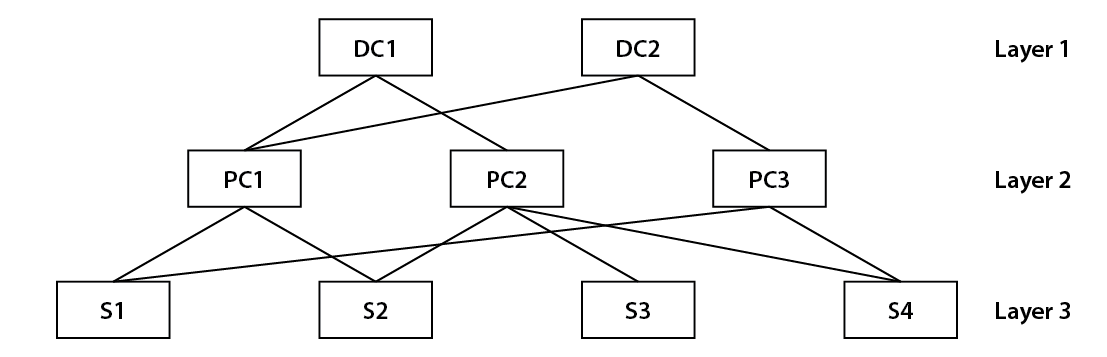
\includegraphics[scale = 0.75, angle = 0]{figures/Formalisation-04}
\caption{Example representation of a belief system with the three layers and several links between the layers. Not all possible causal relations are represented.}
\label{fig:Formalisation-04}
\end{figure}

Each agent has an attribute called \texttt{beliefHierarchy}. This attributes contains two parts as mentioned previously: the agent’s own belief hierarchy and the perceived hierarchies of all other agents in the model. It can be written as follows:

\begin{equation}
beliefHierarchy = [own_{hierarchy}, others_{hierarchy, n}]
\end{equation}

where $n$ represents the number of agents present in the model.

To further specify the hierarchy of the agent considered, the following can be said:

\begin{equation}\begin{split}
own_{hierarchy} &= [issues_k, causal\text{ }relations_l]\\
issues &= [state, aim, preference, awareness]
\end{split}\end{equation}

where $k$ defines the number of issues present in the belief hierarchy structure and $l$ the number of causal relations.

And it is also possible to specify the structure used to saved the perceived knowledge of the belief of the other agents:

\begin{equation}\begin{split}
other_{hierarchy} &= [issues_k, causal\text{ }relations_l]\\
issues &= [state, aim]
\end{split}\end{equation}

In both cases, the issues are specified with deep core issues first, policy cores following and ending with secondary issues. The causal relations are specified in the following example order: DC1-PC1, DC1-PC2, DC2-PC1, DC2-PC2, PC1-S1, PC1-S2, .... The state, preference and causal relation parameters are then specified on the interval of [-1, 1]. The preference is a percentage based parameters and is therefore calculated to be a number on the interval [0, 1].

%- PARAMETERS - The policy network
\subsection{Policy network}

The policy network is the network that links all agents within a subsystem. This network is composed of links with the following attributes: 

\begin{enumerate}
\item A \emph{policy network link} is represented as a 7-tuple \texttt{link = (agent1, agent2, awareness, awarenessDecay, conflictLevel)} where \texttt{agent1} and \texttt{agent2} are the agents at the end of a link, \texttt{awareness} is the awareness value, \texttt{awarenessDecay} is the decay value at which the awareness diminishes per time interval and \texttt{conflictLevel} is the conflict level characterising the relation between two agents for specific issues.

\item The \emph{awareness} value can take three main values. The value -1 refers to the fact that both agents are not aware of each other’s existence. They cannot network together without external introduction from a third party. For the value 0, the actors have no connection but know each other exist. They cannot network together until they have raised their awareness level to a non-negative value through networking actions. Any positive integer relates the value of awareness between the two agents. The awareness is given on the interval $]0,1]$. Note that awareness is relative amongst all links. The policy network links between policy makers can never be -1 as policy makers are public figures. Furthermore, a link cannot be downgraded to -1, it can only start at -1. As the awareness decays over time at a specific rate, there are several actions or events that can lead to a growth or stop the decay in the awareness between two agents. This is detailed later on.

\item The \emph{awareness decay} is represented by a 3-tuple \texttt{(value, time)} where \texttt{value} is the current value of the decay coefficient and \texttt{time} is a countdown. This countdown is by default set at 0, at which point decay of the awareness will happen. The countdown can be set at different values depending on actions that agents performed. The countdown will then go down to 0 every tick by 1. Whenever the countdown is not at 0, the decay is stopped.

\item The \emph{conflict level} parameter is determined for each agent for each issue's aim and state and for causal relations. Note that the conflict level between two agents will be difference depending on which agents is considered as the conflict level is obtained based on the perception of another agent's beliefs. The conflict level is therefore given as a 2-tuple for each link: \texttt{(agent 1, agent 2)}. Then for each agent, the conflict level is defined per issue for the state and then for the aim, and all causal relations. The conflict level is then calculated using:

\begin{equation}\begin{split}
CW \text{ }conflict \text{ } level_{n,n_m} &= |CW_n - CW_{n_m}| \\
aim \text{ } conflict \text{ } level_{n,n_m} &= |A_n - A_{n_m}| \\
state \text{ }conflict \text{ } level_{n,n_m} &= |S_n - S_{n_m}|
\end{split}\end{equation}

where $CW$ the causal weight, $A$ is the aim, $S$ is the state, $n$ is the agent for which the conflict level is calculated and $n_m$ is the perceived belief of agent $n$ on agent $m$ for that specific issue.

The resulting value is then formatted into a coefficient to be used in the grading of actions as is shown later on. When the result obtained is between 0 and 0.25, the conflict level is considered to be low, the coefficient is then set at 0.75. When the result obtained is between 0.25 and 1.75, the conflict level is considered to be medium, the coefficient is set to 0.85. Finally for a result higher than 1.75, the conflict level is considered high and the coefficient is set to 0.95. Note that both the intervals and the resulting coefficients can be varied by the modellers during experimentations to better tailor their model to their case studies.

\end{enumerate}

%-
\paragraph{Network upkeep and maintenance}

Each agent must maintain his/her policy network. For this, 20\% of agent’s resources can be used. The agents are allowed five actions, each time spending 4\% of the total amount of resources for each action. The order in which agents are selected to perform their network actions is random. These numbers can be changed by the modellers for the purpose of theirs cases.

Two strategies are differentiated for these actions. The modellers have to specified which strategy each agent uses in the model inputs. They are given as follows:

\begin{enumerate}
\item Largest network strategy - the agent will look into increasing his/her network as much possible:
	\begin{enumerate}
	\item The agent first wants to keep all links active. Any link that is below 30\% awareness level will be targeted for action. The lowest, but still above 0, will have priority.
	\item If all links are above 30\% awareness, the agent will look into introducing new links which had 0\% awareness. The priority is placed on the link with agents with the closest beliefs.
	\item If there are still resources left after step 1 and 2 are complete, the agent will maintain the links with the lowest awareness level in the network.
	\end{enumerate}

\item Focused network strategy - the agent will focus on maintaining a network of agents sharing its beliefs: (note that when it is stated similar belief, this relates to the problem that the agent is advocating for and no other issue)
	\begin{enumerate}
	\item The agent will look first for link where an agent with a similar belief (one of the agents has his belief within 0.2 of the other agent's aim belief) or higher belief level and with a awareness which is lower than 70\%. The agent will prioritise based only on the awareness level as long as the belief criteria is met.
	\item If no link qualifies, then the agent will seek to introduce new links in his/her network. The agent will select agents that have a similar belief or higher belief level.
	\item If both step 1 and 2 are met, the agent will look into maintaining an awareness level above 70\% for links still in service. The priority is put on the links with the lowest awareness value.
	\item If all previous steps are met, then the agent will simply look for new links with the priority placed on agents sharing his/her beliefs.
	\end{enumerate}
\end{enumerate}

The different actions mentioned above are performed as follows:

\begin{itemize}
\item An agent can increase the awareness in a network link if he feels the awareness level is too low. This awareness maintenance is dependent on three main parameters: the resources spent and the affiliation of both agents. The total increase in awareness for such an actions is calculated as:

\begin{equation}
awareness := awareness + resources \cdot affiCoef_{Aff_n,Aff_m}
\end{equation}

where the $affiCoef_{Aff_n,Aff_m}$ is the weight related to the affiliation of the two agents. If they share the same affiliation, then it is equal to 1.

\item Agents can also establish links with other agents for which they know they exist. This action can only be performed when the \texttt{link.awareness} parameter is equal to 0.

If this is the case, then the awareness can be increased through the spending of resources. The new awareness level is then calculated similarly to the awareness maintenance but with a small malus to account for the initial investment costs. The equation is given as follows:

\begin{equation}
awareness := resources \cdot affiCoef_{Aff_n,Aff_m} \cdot 0.5
\end{equation}

\item The notion of similar belief is defined as agents being close for the aim on issues at the policy core level. There are several steps to seek agents with similar beliefs:

\begin{enumerate}
\item Seek all links with awareness equal to 0 or higher and select their associated agents.
\item Select the aim parameter of the problem of the original agent.
\item For each associated agent, check its aim parameter for this same problem issue.
\item Calculate the difference of the parameter between the original agent and the associated agent for this issue.
\item Rank all differences from lowest to highest where the lowest is considered to be an agent of similar beliefs.
\end{enumerate}

This ranking is calculated based on the agent’s partial knowledge of other agent’s beliefs.
\end{itemize}

%- PARAMETERS - The affiliation network
\subsection{Affiliation network}

The affiliation network is a network that looks at the political affiliation of the different actors. Its links are represented as a 3-tuple given by \texttt{(affiliation1, affiliation2, affiCoef)} where \texttt{affiliation1} and \texttt{affiliation2} are the affiliations that are connected by the link and \texttt{affiCoef} represents the influence that an actor with an affiliation 1 can have on an actor with affiliation 2. The \emph{affiliation coefficient} is given on the interval $[0,1]$.

%- Actions
\subsection{The actions - Policy Makers}

There is a set of actions that policy maker agents can perform within the model. These actions are individual framing where the causal relations are the target of the influencing action, aim influence where the issue aim is the target of the influencing acton and state influence where the issue state is the target of the influencing action. These three times of actions are presented below in more details.

When selecting an action, the agent will perform all possible actions and calculate the likelihood grade of all actions. The agent will then select the action with the highest grade as the action to be implemented. The calculation of the likelihood of perfuming an action is mostly based on the beliefs of the influencing agent and his perception of the beliefs of the influenced agent. However, the actual impact of the action is based on the beliefs of the influencing agent and the beliefs of the influenced agent. This is an important difference that can sometimes justify why meaningless actions are performed. This can be due to a false perception of another agent’s beliefs.

%0
\paragraph{Individual framing}

The agents can attempt to influence the causal relation belief of other agents. This is an individual framing action. For this action, all causal relations related to the issue selected by the agent are considered. The likelihood to perform such an action depends on several parameters which are outlined below:

\begin{equation}\label{eq:likelihoodFraming}
G_{CW, n_m} = conflictLevel_{CW, n, m} \cdot affiCoef_{Aff_n,Aff_m} \cdot awareness_{n,m} \cdot actionWeight_{n,m}
\end{equation}

where $G$ stands for the grade, $n$ is the influencing agent, $m$ is the influenced agent. $n_m$ is the perfection of the beliefs of the influenced agent by the influencing agent and $CW$ is the causal weight of the causal relation

If this action is selected, as it has the highest grade, then the impact of the action on the beliefs of the influenced agents is given by:

\begin{equation}\label{eq:impactFraming}
CW_{m} := CW_{m} + \left(CW_{n} - CW_{m} \right) \cdot resources \cdot affiCoef_{Aff_n,Aff_m}
\end{equation}

%0
\paragraph{Individual action - Aim change}

The agents can also attempt to influence the aim beliefs on the different issues of the hierarchy of other agents. The likelihood that such action be performed is obtained in a similar way as shown below:

\begin{equation}\label{eq:likelihoodAimChange}
G_{A, n_m} = conflictLevel_{A, n, m} \cdot affiCoef_{Aff_n,Aff_m} \cdot awareness_{n,m} \cdot actionWeight_{n,m}
\end{equation}

The impact of such action is then calculated with:

\begin{equation}\label{eq:impactAimChange}
A_{m} := A_{m} + \left(A_{n} - A_{m} \right) \cdot resources \cdot affiCoef_{Aff_n,Aff_m}
\end{equation}

%0
\paragraph{Individual action - State change}

Similarly to the influence on the aims of an agent, the states can also be influenced. The likelihood of such an action being performed is given as follows:

\begin{equation}\label{eq:likelihoodStateChange}
G_{S, n_m} = conflictLevel_{S, n,m} \cdot affiCoef_{Aff_n,Aff_m} \cdot awareness_{n,m} \cdot actionWeight_{n,m}
\end{equation}

And the impact is calculated as follows:

\begin{equation}\label{eq:impactStateChange}
S_{m} := S_{m} + \left(S_{n} - S_{m} \right) \cdot resources \cdot affiCoef_{Aff_n,Aff_m}
\end{equation}

%0
\subsection{Preference calculation (issues)}

As mentioned earlier on, the policy maker has a limited attention span. This results in having to select one issue at a time for which (s)he thinks is the most urgent issue. This urgency is defined as the preference of an agent and is calculated for each layer in the belief hierarchy of the policy maker. Two cases must be distinguished for calculating this urgency: whether the layer considered is at the top or in the rest of the hierarchy. The preference is calculated for each issue and the sum of all preferences on each layer must be equal to 1.

\paragraph{Preference calculation for the principle beliefs}

For the top layer which is composed of the principle beliefs, the preference is calculated differently than for the other layers. This is because these beliefs are on the highest layer and can therefore not be connected to higher layers with causal relations. The calculation of the preference for each issue is given by:

\begin{equation}
P_i = \frac{ |A_i - S_i|}{\sum_{j=1}^n |A_j - S_j|}
\end{equation}

where $j$ is defined at the number of principle belief issues and $i$ characterises the principle belief issue being selected for the calculation.

\paragraph{Preference calculation for the policy core and secondary beliefs}

The preference calculation for the other layers in the belief hierarchy is adapted to include the causal relations that link these layers to higher up layers. This calculation applies to the policy core beliefs which are in the middle of the hierarchy and the secondary beliefs at the bottom.

To calculate the preference, the gap between aim and state for the issues is considered along with the impact of the causal relation on the gap of the issue on the above layers. The causal relations are not always helping bridge the gap between the aim and the state of issues on a higher layer. If this is the case, then the causal relations are not considered within the calculation as there effort is counter productive within the mind of the agent. The resulting equation that can be used to calculate the preference for these layers is given by:

\begin{equation}\label{eq:preference2}
P_k= \frac{ |A_k - S_k| + \sum_{j=1}^n |CW_j \left( A_j - S_j \right)|}{\sum_{l=1}^p \left[ |A_l - S_l| + \sum_{j=1}^n \left|CW_{j,l} \left( A_{j,l} - S_{j,l} \right) \right| \right]}
\end{equation}

The sums only include these terms if $CW_j$ and $\left( A_j - S_j \right)$ have the same sign. If it is not the case, these terms are not considered. And where $p$ is defined at the number of policy core issues, $k$ characterises the policy core issue being selected for the calculation, $j$ specifies the associated deep core and $CW$ represents the weight of the causal relation.

Based on these preferences obtained, the agent will select one issue to advocate for as mentioned earlier. For each layer, the agent will choose the issue with the highest preference. This is the case for each layer. The actions that the agent will then perform will be to influence other agents on the issue they have selected specifically.

%0
\subsection{Partial knowledge and awareness decay}

The likelihood of performing an action is based almost entirely on the perception of an agent on another agent’s beliefs. This is also referred as the partial knowledge of an agent. This partial knowledge is the representation that agents have of other agent’s beliefs. To perform better informed decisions, the agents must update their partial knowledge about other agents.

This update is performed after two agents have interacted with one another. When an action is performed, both agents have come into contact and have learnt about each other’s beliefs on the issue they have interacted on. This allows them to gain knowledge about the other’s belief. Therefore, for each action implemented, each agent will have access to the belief of the other agent concerning the issue influenced during the action. This access is not complete, the agents will gain the beliefs of the other agent with a small uncertainty amount.

Furthermore, because the two agents have interacted, their awareness of one another will not decline. It is therefore kept at the current level for several time steps. Only after these time steps have passed and if both agents have not interacted since, the decay of their awareness of one another will continue.

%- PARAMETERS - The agenda parameters	
\subsection{Agenda and agenda selection}

The \emph{agenda} is a 1-tuple given by \texttt{agenda = (issue, problem, policy)} where \texttt{issue} is the issue that is placed on the agenda by the policy makers, \texttt{problem} is the problem selected and \texttt{policy} is the policy selected by the policy makers. Note that the problem and policy attributes are only considered within the three streams theory, they are left empty within the common core.


To constitute the agenda, an issue has to be chosen for the entire subsystem. For this two methods are proposed which can yield different results. The first method considers all the top issues as graded by the policy makers. They are affected by their normalised resources. The grade of each issue is the sum of all agent's resources which have chosen that issue as their preferred issue. Whichever issue has the highest grade becomes the issue on the agenda.

The second method used for the ranking and selection of the issues is similar to the first one. The difference is that here all issues are taken from each policy maker. They are then weighed all together (and not simply the issues at the top of the ranking of each agent). This approach is meant to represent a different approach to the power dynamics in the model. The grade for each policy is then obtained as:

\begin{equation}
rankingGrade = \sum_{i=0}^n \left( \frac{1}{P_{rank}} \cdot resources_n \right)
\end{equation}

where $n$ is the number of agents and $P_{rank}$ is the ranking of the policy for that agent.

The issue with the highest grade is then taken as the issue for the agenda.

%- Actions
\subsection{The actions - Policy entrepreneurs}

The actions of the policy entrepreneurs are the same as the ones presented for the policy makers. The only difference is that the policy entrepreneurs cannot choose the agenda.

%- Actions
\subsection{The actions - External parties}

As mentioned in the conceptualisation, the have a more complex roles that the policy makers and entrepreneurs. They have different and similar actions to these actors. Their first role is to transmit the states of the world to the different agents in the model. This role is passive and does not require any resources. The second role is to blanket influence the electorates. For this 20\% of the resources of the external parties are used spent in interval of 10\%. The final role is an influencing role. Three actions are then available to the external parties: blanket framing, blanket aim influence and blanket state influence. 100\% of the resources are allocated for this actions to be spent in intervals of 10\%. For this all actions are graded and the one that is most likely to be considered is performed.

%0
\paragraph{Transmitting the states}

The states of the issue in the hierarchy beliefs of all agents are updated based on the information they get from the external parties. These external parties have access to the full and real states of the world. They can obtain these states from the truth agent which has the complete set of the states for each issue directly from the world. Each external party selects states that (s)he finds interesting to transmit them to other active agents. This transmission of the states can be affected by the political affiliation of the agents as agents of different affiliation are unlikely to fully trust one another. The equation used to calculate this update of the states is given below:

\begin{equation}
S_{agent} := S_{agent} + \frac{1}{n} \sum_{i=1}^n \left( \left(S_{EP_n} - S_{agent} \right) \cdot affiCoef_{Aff_n,Aff_m} \right)
\end{equation}

where $S$ stands for the issue state, $n$ is the number of external parties, $EP$ stands for external parties and $affiCoef_{Aff_n,Aff_m}$ is the affiliation related weight. The affiliation coefficient is the one that relates the affiliation of the agent and the affiliation of the external party selected. If an external party has not selected that specific state, then (s)he will not be able to provide the state for that issue. Furthermore, the external parties will only transmit the states to agents within their network. This can lead to some agents lacking states for specific issues because of the composition of their policy network.

%0
\paragraph{Electorate influence}

The external parties can also influence the goals of the electorate. This is done following the same template the goal influence of the policy makers and entrepreneurs. The only difference is that it is once again blanket influence which means that all electorate agents are affected at once. Note that because the external parties have a limited attention span, they can only influence the electorates on the issue they have selected. The impact of this influence is given by the following equation:

\begin{equation}
A_{El, i} := A_{El, i} + \left(A_{n, i} - A_{El, i} \right) \cdot affiCoef_n \cdot resources \cdot \frac{1}{nEl}
\end{equation}

where $n$ is the external party, $i$ is the issue and $nEl$ is the number of electorates.

%0
\paragraph{Blanket framing}

The external parties can also attempt to influence the understanding of the world of other external parties, the policy makers and policy entrepreneurs. The external parties perform such influence on all agents at the same time which leads to this action being called blanket framing. The overall calculation of the likelihood of performing such an action is similar to what was presented for the framing action of the policy makers. The impact is also similar but spread amongst all agents. Such action can only happen on the agents that are within the policy network of the external party. All causal relations related to the issue selected by the external party can be influenced.

The likelihood of performing a blanket framing action is calculated as follows:

\begin{equation}\label{eq:likelihoodBlanketFraming}\begin{split}
G_{CW, n_m} &= conflictLevel_{CW, n, m} \cdot affiCoef_{Aff_n,Aff_m} \cdot awareness_{n,m} \cdot actionWeight_{n,m}\\
G_{CW, n} &= \sum_{m = 1}^{nagents-1} G_{CW, n_m}
\end{split}\end{equation}

where $CW$ is the causal weight selected, $n$ the external party performing the framing, $m$ the affected agents considered and $nagents$ the total number of agents.

The impact of this action is then calculated for each agent using:

\begin{equation}\label{eq:impactBlanketFraming}
CW_{m} := CW_{m} + \left( CW_{n} - CW_{m} \right) \cdot resources \cdot affiCoef_{Aff_n,Aff_m} \cdot \frac{1}{nagents}
\end{equation}

%0
\paragraph{Blanket aim influence}

The external parties can also attempt to influence the aims of the other agents. This is done on all agents at once similar to the blanket framing.

The likelihood of performing a blanket aim influence action is calculated as follows:

\begin{equation}\label{eq:likelihoodBlanketFraming}\begin{split}
G_{A, n_m} &= conflictLevel_{A, n, m} \cdot affiCoef_{Aff_n,Aff_m} \cdot awareness_{n,m} \cdot actionWeight_{n,m}\\
G_{A, n} &= \sum_{m = 1}^{nagents-1} G_{A, n_m}
\end{split}\end{equation}

where $A$ is the aim of the issue selected, $n$ the external party performing the framing, $m$ the affected agents considered and $nagents$ the total number of agents.

The impact of this action is then calculated for each agent using:

\begin{equation}\label{eq:impactBlanketFraming}
A_{m} := A_{m} + \left( A_{n} - A_{m} \right) \cdot resources \cdot affiCoef_{Aff_n,Aff_m} \cdot \frac{1}{nagents}
\end{equation}

%0
\paragraph{Blanket state influence}

Finally, the external parties can attempt to influence the states of the other agents. This is done on all agents at once similar to the blanket framing.

The likelihood of performing a blanket framing action is calculated as follows:

\begin{equation}\label{eq:likelihoodBlanketFraming}\begin{split}
G_{S, n_m} &= conflictLevel_{S, n, m} \cdot affiCoef_{Aff_n,Aff_m} \cdot awareness_{n,m} \cdot actionWeight_{n,m}\\
G_{S, n} &= \sum_{m = 1}^{nagents-1} G_{S, n_m}
\end{split}\end{equation}

where $S$ is the state of the issue selected, $n$ the external party performing the framing, $m$ the affected agents considered and $nagents$ the total number of agents.

The impact of this action is then calculated for each agent using:

\begin{equation}\label{eq:impactBlanketFraming}
S_{m} := S_{m} + \left( S_{n} - S_{m} \right) \cdot resources \cdot affiCoef_{Aff_n,Aff_m} \cdot \frac{1}{nagents}
\end{equation}



%-
\subsection{Electorate passive action on policy makers}

The policy makers are passively influenced by the electorate. Each electorate has a certain affiliation to which policy makers are also related. Each policy makers' issue aim will be influenced by their respective electorate. This happens as a passive effect where the issue aims of the policy makers slowly progress towards the issue aims of the electorate. The equation to calculate the change in the aim of the policy maker is given as follows:

\begin{equation}
A_{PM} := A_{PM} + \left(A_{El} - A_{PM} \right) \cdot 0.001 \cdot \left| A_{El} - S_{El} \right|
\end{equation}

where $El$ stands for electorate and $PM$ for policy maker. Note that this is only performed for the issues of the policy maker for agents with matching affiliations. Furthermore, the value 0.001 is arbitrary and can be changed by the modeller depending on the case study.

%- PARAMETERS -  The policy instruments
\subsection{Policy instruments}

The policy instruments are measures that can are chosen by the policy makers to impact the real world. Policy entrepreneurs and external parties can also influence the policy makers in their choices. To assess the different policy instruments, the different active agents assess the impact of these instruments on the secondary issues in their belief hierarchy. These instruments have an impact on the gap between the states and the aim of each of these issues. The policy instruments can be described as follows:

\begin{enumerate}
\item A \emph{policy instrument} is represented as a 7-tuple \texttt{(name, impact, change, layer, children, awareness, feedback)} where \texttt{impact} is related to the impact of the policy on a specific issue, \texttt{change} is the objective change expected in the world due to this policy, \texttt{layer} corresponds to the layer in the instrument hierarchy (when used), \texttt{children} corresponds to the instruments linked to the selected instrument in the instrument hierarchy, \texttt{awareness} is related to the availability of the policy for a specific agent and \texttt{feedback} is related to the expected model feedback from the implementation of the policy considered.

\item The \emph{impact} of a policy instrument is given as a 2-tuple: \texttt{(issue, impact)} where \texttt{issue} defines which of the secondary issues is affected and \texttt{impact} specifies by how much.

\item The \emph{change} due to a policy instrument is the subjective representation of the impact of the policy instrument. These are the actual changes that will occur in the world with the implementation of the instrument. They are defined by the modeller and are fully independent on the agents.

\item The \texttt{layer} and the \texttt{children} are both parameters that related to the three streams theory. They are therefore outlined in that section and are left empty for the common core.

\item The \emph{awareness} parameter defines whether a certain policy instrument is known in a specific subsystem. This parameter is related to the diffusion theory and is further outlined in the section dealing with the diffusion theory.

\item The \emph{feedback} parameter contains the feedback effects as defined by the modeller. This parameter is related to the feedback theory and is further explained in the feedback theory section.
\end{enumerate}

%-
\subsection{Preference calculation (instruments)}

Similarly to the agenda setting round, in the policy formulation round, the agents have a limited attention span. They can therefore only select one policy instrument at a time. The calculations used to select these instruments are slightly different than the ones in the agenda setting. They are shown below

%0
\paragraph{Preference calculation}

The preference calculation of the secondary issues within the context of a policy formulation rounds are tweaked from the calculation presented in the agenda setting round. The main reason is that for the policy formulation, the number of issues considered is narrowed down by what is on the agenda. The agents can therefore only consider issues in the secondary belief layer that have a direct effect, according to their beliefs, on the issue that is on the agenda. All other issues are not included within the preference calculation. For the rest, \autoref{eq:preference2} is still used to calculate the preferences of the different issues for each agent according to their own beliefs.

%0
\paragraph{Instrument selection calculation}

Once the preferences for the different secondary issues have been attributed, it is possible to look at the preference of the instruments. These are used by the agents to assess the instruments and select the one they find most important. The equation that is used to calculate the preference of the different instruments is provided below. Similarly to the calculation of the preferences in the belief hierarchy, only instruments with impacts that have the same sign as the belief gap (aim minus state for a specific issue) are considered. The other instruments are counter productive and are therefore directly excluded from considerations.

\begin{equation}
P_i = \sum_{j=1}^n \left[ impact_j \cdot \left( A_j - S_j \right) \cdot P_j \right]
\end{equation}

where $n$ is the number of impacts this policy instrument has, and $j$ represents the secondary issue and the associated impact of the policy instrument on that issue.

Once all the preferences have been calculated, the agent will select the instrument with the highest preference. This will help define the actions that each agent can perform. Because no actions can be performed on the instruments directly, the agent will be able to perform actions on all issues directly related to the instrument and all causal relations which link the issue on the agenda and the issues related to this instrument. The likelihood and the impact of the actions are calculated in the same way as was shown previously. The aim here for the agents is to convince other agents that the instrument’s impact is as high as they perceive because their causal relations, aims and states beliefs are similar.

%-
\subsection{Policy instrument selection and implementation}

Similarly to the agenda setting round, the policy makers are the agents that can selected a policy instrument. Additionally, they will decide if a policy instrument should be implemented. This is done through one of two strategies which can be chosen by the modeller and which rare presented below.

%0
\paragraph{Unanimity}

If unanimity is required, all policy makers must have selected the same policy instrument for it to be implemented. If this is not the case, the instrument will not be implemented and the round will close without a definitive output.

%0
\paragraph{Majority}

If a majority is required, 50\% plus one policy maker must select the policy instrument for it to be implemented. The resources of the different policy maker has no impact on this majority as it had in the agenda setting round. If a majority cannot be found, the policy instrument will not be implemented.

%-
\subsection{External events}

The external events that are considered are external events that affect the agents. External events that would affect the world such as a flood for a hydrological model are of no interest and considered out of scope of this report. However, the impact on the model such as a change in the electorate composition due to the flooding is of interest.

The following is a non-exhaustive list of potential external events which the modeller could use.

\begin{enumerate}
\item An election - this would create a change in the electorate representation parameter which would in turn lead to different resources allocation for the policy makers.
\item The introduction of a new issue - a new issue could be introduced to the system or to a subsystem. This would affect the knowledge parameter for an issue for all agents present in the model.
\item Resources shift - a shift in the resources distribution due to an external event could be modelled. The way the resources are attributed could be modified to simulate a crisis situation were resources are scarce. This could also be modelled as a reduction in the possibility of actions (increasing the amount of resources that is spent per action).
parameter would be changed.
\item Policy network shifts - change in the awareness parameter of specific network links.
\item Affiliation network shift - change in the affiliation coefficient parameter that defines the interaction possibilities between two different political affiliations
\end{enumerate}

%-
\subsection{The model cycle}

For this formalisation, it is assumed that the different rounds are performed consecutively. First the agenda setting rounds are performed, then the policy formulation rounds and finally the real world. A further assumption is to assume that there is only one round of each of these steps is performed. This leads to a 3-step model with an agenda setting step, a policy formulation step and a world simulation step. The agenda which is obtained at the end of the agenda setting helps defines what the agents will be interacting about within the policy formulation.

This has several consequences. The first one is that the beliefs hierarchy of the agents must be a three-layer hierarchy. At the top are the principle beliefs, then in the middle the policy core beliefs and at the bottom the secondary beliefs. Within the agenda setting, the agenda decide on an agenda issue from the second layer, the policy core issues. Within the policy formulation, the agents select instruments which are related to the third layer.

The steps used to mode this approach are then detailed as follows:

\begin{enumerate}
\item World round:
	
	\begin{enumerate}
	\item \emph{World simulation:} The world which is an exogenous party to the model or an internal technical model are run to provide inputs for the next step.
	\item \emph{Trigger of external events:} Any event that the modeller decides to implement are activated at this stage of the model cycle.
	\item \emph{Update of the truth agent:} The technical output is converted into normalised data fitting with the issues present in the belief tree. These are placed in the truth agent's $S$ parameters.
	\item \emph{Electorate action on policy makers}
	\item \emph{Transmission of the states:} The external parties select their states of interest from the truth agent and pass the information to the agents within their policy network.
	\end{enumerate}
	
\item Agenda setting round:


	\begin{enumerate}
	\item \emph{Preference calculation (issues):} Each agent calculates the preference for their principle and policy core beliefs. The agents then each select an issue that (s)he will advocate for in his/her policy core beliefs based on the preferences calculated.
	\item \emph{Agent interactions:} 

		\begin{enumerate}
		\item \emph{Resources received:} Each active agent receives its resources based on his/her political affiliation.
		\item \emph{Network upkeep or maintenance}
		\item \emph{Belief influence actions:} All active agents perform their respective actions. The order in which the agents perform their actions is made random to not favour agents with first or last actions.
		\end{enumerate}

	\item \emph{Preference calculation (issues):} Each policy maker updates his preferences for his principle and policy core beliefs. This update of the preference is necessary to take into account the changes that might have occurred as a results of the agent interactions. Each policy makers choose the issue with the highest preference as their issue of preference.
	\item \emph{Agenda selection}
	\end{enumerate}
	
\item Policy formulation round:

	\begin{enumerate}
	\item \emph{Preference calculation (instruments):} Each agent update his preference for his secondary beliefs based on the issue on the agenda. Each agent then selects a policy instrument that (s)he will be advocating for.
	\item \emph{Agent interactions:} 

		\begin{enumerate}
		\item \emph{Resources received}
		\item \emph{Network upkeep or maintenance}
		\item \emph{Belief influence actions}
		\end{enumerate}

	\item \emph{Preference calculation (instruments):} Each policy maker upgrades their policy instrument preferences after the interaction step.
	\item \emph{Policy instrument implementation} 
	\end{enumerate}
	
\item \emph{The model advances:} The clock is advanced to the next tick. Programming of ticks actions are also performed (data collection, policy network awareness decay, …).

\end{enumerate}

% THE THREE STREAMS THEORY
\section{Three streams theory}

The three streams theory introduces a number of changes and additional concepts to the common core. These are detailed here. The first important addition and change is related to the policy instruments which are now assembled in an instrument hierarchy. Another change comes with the fact that the agent now must choose between a policy and a problem based on the calculated preference. Furthermore, because agents are not able to select policies, they are provided with an additional action. Finally, the agents can assemble in teams. This requires an algorithm for the creation of such teams and it brings in more actions that the actions can perform within and outside of their teams.

%-
\subsection{The policy instruments}

As explained in the conceptualisation, the actors now each have an instrument hierarchy similar to their belief hierarchy. To formalise this hierarchy, two attribute within the policy instruments are activated. These are the layer and children attributes. The layer attribute defines in which layer of the hierarchy the instrument fits. These layers are related to the layers present in the belief hierarch. This means that policy instruments in the second layer of the instrument hierarchy will have an impact on the issues which are in the second layer of the belief hierarchy. The children attributes helps understand which instruments are related across the different layers. This is defined by the modeller and is useful to navigate from one round to another. When a certain instrument is placed on the agenda from the second layer, then only his children present in the third layer can be considered by the agents. All other instruments are considered irrelevant. A representation of the instrument hierarchy is given in \autoref{fig:Formalisation-09}.

\begin{figure}
\centering
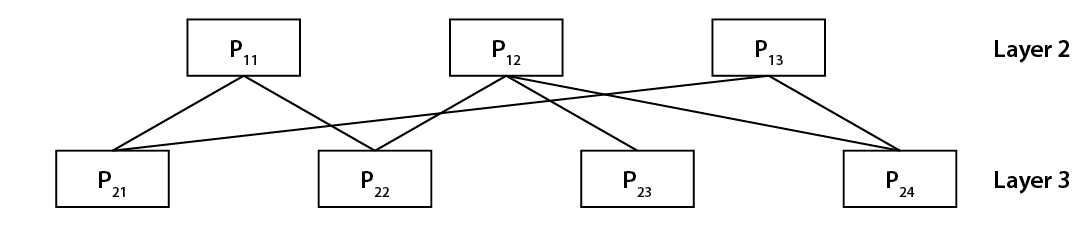
\includegraphics[scale = 0.75, angle = 0]{figures/Formalisation-09}
\caption{Instrument hierarchy representation with the two layers.}
\label{fig:Formalisation-09}
\end{figure}

There is an additional change that occurs within the policy instruments. The impact is not objective anymore. The impact is now a subjective parameters very much like the states and aims for the issues in the belief hierarchy. This is important as the agents will be able to influence other agents on their beliefs of the impact of the different instrument available to them.

%-
\subsection{Preference calculation (problems and policies)}

As mentioned within the conceptualisation, the agents can now select a policy or a problem. For that they must grade all problems and policies in every layer. They can then select the policy or problem that has the highest grade.

%0
\paragraph{Problem and policy preference calculation}

The problems and policy grades are obtained differently. The problems are based in the belief hierarchy and their grades are calculated similarly to the issues in the common core. The equation is given as:

\begin{equation}
G_{prob, i} = \left( A_i - S_i \right) + \sum_{j=1}^n \left| CW_j \left( A_j - S_j \right) \right|
\end{equation}

where $i$ corresponds to the policy core considered and $j$ the related deep core issues.

The policy instrument are assessed on their impact on the different gaps in their associated issues in the belief hierarchy. The equation used to calculate their grades is given by:

\begin{equation}
G_{policy, i} = \sum_{i=1} \left( A_i - S_i \cdot I_i \right)
\end{equation}

where $i$ corresponds to the policy core affect by the policy selected and $I$ is the impact expected from the policy.

Once all possible policies and problems have been graded, the agent will select the one with the highest grade. Then the process is repeated again but for the associated issues. This is done with only problems related to the policy selected if a policy was selected first or with the policies related to the problem selected if the problem was selected first.

The actions that the agents will perform will be based on whether they first selected a problem or a policy. These actions are detailed in a subsequent section.

%0
\paragraph{Agenda and agenda selection}

Within the three streams approach, the agenda selection is a little different than for the common core. The agenda is now composed of two parts: a problem and a policy. The issue attribute of the agenda is left empty. The rest is similar to the common. The problem selected for the agenda is the most popular problem for all agents considering their respective resources while the policy chosen is the most popular policy amongst all agents also considering their resources.

%0
\paragraph{Policy instrument selection and implementation}

For the policy formulation round, the procedure to select and implement a policy instrument is similar to the common core procedure. The policy chosen by all policy makers is considered. If a policy is beyond the threshold set but the modeller for implementation, the policy will be implemented. The problem chosen by the policy makers is not taken into account.

%-
\subsection{The actions (active agents)}

The influencing actions that the agents can perform are mostly similar to the ones in the common core. The main difference is that all their actions are performed on the problems if they have first selected a problem. The policy makers and entrepreneurs can perform framing, state influence and aim influence actions on other agents based on the problem they have selected in their belief hierarchy. The external parties can perform their blanket framing on other agents and blanket aim influence on the electorate. This is also based on the problem they have each selected.

For the agents that have selected a policy, an additional action is added. This action is an action that influences the impact beliefs of the policy instrument selected by the agent. For all agent, this action replaces the framing or blanket framing action. The aim and state influence actions remain the same. The likelihood of performing each action is calculated. Whichever action is most likely to be performed is implemented with a certain calculated impact.

The likelihood of performing a policy action is given as follows:

\begin{equation}\label{eq:likelihoodImpact}
G_{I_{issue}, n_m} = conflictLevel_{I_{issue}, n, m} \cdot affiCoef_{Aff_n,Aff_m} \cdot awareness_{n,m} \cdot actionWeight_{n,m}
\end{equation}

where $n$ is the agent performing the action, $m$ is the agent on which the action is performed, $I$ stands for the impact that the action has on the mentioned issue. Note that if the instrument has an impact on four separate issues, then the agent will assess the likelihood of influencing each of the four impacts contained in that policy instrument.

The impact of the action is then given as follows:

\begin{equation}\label{eq:impactImpact}
I_{m, issue} := I_{m, issue} + \left( I_{n, issue} - I_{m, issue} \right) \cdot resources \cdot affiCoef_{Aff_n,Aff_m}
\end{equation}

where $n$ is the agent performing the action, $m$ is the agent on which the action is performed.


%-
\subsection{The teams}

As mentioned in the conceptualisation, the three streams theory includes the concept of teams. This concept is formalised within this section.
Teams contain a number of agents that feel they share their beliefs for a specific issue. A team is therefore given as a 6-tuple written as: \texttt{(team ID, lead, members, issue, creation, resources)} where \texttt{lead} is the leader of the team (the agent that created the team), \texttt{members} is the list of members that are part of the team, \texttt{issue} is the policy issue that the team is advocating for (policy or problem), \texttt{creation} is the time at which the team has been created and \texttt{resources} consists of the resources at the disposal of the team to perform actions. The resources are calculated as the sum of all the members belonging level.

%0
\paragraph{Agent-team actions}

The agent-team actions are all actions that each agent performs to either decide to join or create a team. It also consists of actions related to the disbanding of teams and the checking that the team requirements are still met. Each agent goes through all of these actions each tick. Each agent can only be part of one team at a time in the agenda setting process and one team in the policy formulation process. Note that all actives agents can be part of teams. The following list presents the different actions that are taken in chronological order in which they are performed in the model: start a team, join a team, leave a team, disband a team and calculate belonging level.

%0
\paragraph{Start a team}

An agent that wants to start a team has to consider different requirements. Two different cases have to be considered here: the case where the agent first chose a problem and the case where the agent first chose a policy.

If the agent first chose a problem then the first requirement is that for the secondary issue chosen, the gap between aim and state must be above a certain threshold. This threshold is 0.8 in general but can be set to 0.5 in cases where a change in the magnitude of the state from the previous tick is larger than 0.5 (in case of an external event). This must be the case for all agents if they want to join the team. The second requirement relates to the belief states. For the agenda setting, it is the causal relation between the deep core issue with the highest preference for the starting agent and the policy core issue selected as the problem. For the policy formulation, the causal relation selected is the one relating the problem on the agenda and the secondary issue selected as the problem by the agent. All agents that want to join the team must be within 0.5 of the value of the causal relation for the agent starting the team.

If the agent first choses a policy, then there is a small change in the requirements looked at. The agent still looks at the gap requirement. However the second requirement is now dependent on the impact that the policy has on the secondary issues selected as the problem by the agent that is starting the team. The impact on the associated problem should be within 0.5 for the other agents considered to enter the team.

If both of these requirements are met, then the agents qualifies to join the team. Note that for each agent contacted, the agent starting the team loses 2\% of his resources and the contacted agent loses 1\% of his resources. This is to justify the resources needed for the exchange of knowledge. Furthermore, the agent starting the team will initially assess the other agents based on his knowledge of their beliefs. This leads to the spending of resources. If his perception of the other agent's beliefs are not true, then the agent will not join the team but the resources will have been spent regardless. The resources are also used to gain some information on the beliefs of the other agents. Even though the other agents might not be interested, spending these resources allow the agent to gain knowledge of the beliefs of the other agent within a certain range. Through this exchange of knowledge the agent also provides his own beliefs to the agent being contacted.

The creation of the team requirements are then based on the strategy that the agent is using. Two strategies are considered. The first strategy consists of starting a team with all the agents found that meet the requirements mentioned earlier. The team will then be composed of the maximum number of agents possible. The second strategy consists of starting a team once a certain number of agents has been established to meet the aforementioned requirement.

Upon the creation of a team, all agents that are part of the team are added to the member list. The lead agent of the team is the agent that started the team. Each agent's belonging level is also calculated based on a weighted average of the beliefs of the team on the state of the issue advocated for. Joining a team will also lead to the half of the awareness decay in the links between the agents present in the team, effectively counting as an action.

%0
\paragraph{Join a team}

An agent can join a team if (s)he is not already part of a team. For this, the agent will check the same requirements as when creating a team (gap and causal relation/impact requirements). This is done for the issue of the team (s)he is approaching. For each team that the agent probes, 2\% of his resources are spent. If the requirements are met, then the agent will join the team and be added as a member of the team. The agent is allowed to spend 50\% of his resources for such a search. Once these resources have been depleted or all team have been considered, the agent moves on.

%0
\paragraph{Leave a team}

An agent can leave another team for one reason: because his belonging level is too low. The belonging parameter of the agent is checked every time period. If it descends below 30\% then the agent will automatically leave the team. If the team remaining has less than three agents, it will be disbanded right away. Note that the belonging parameter is updated based on the perception of an agent on another agent's beliefs (partial belief) without full knowledge. This will artificially increase the life of teams. 

%0
\paragraph{Disband a team}

As mentioned earlier, a team will be disbanded if the problem or policy advocated by the team does not match the problem or policy advocated by the lead agent. This can be due to the leader being influenced and having changed his/her preferences. This is checked every five time periods. The second reason for which a team will be disbanded is if the agents present in the team to not meet the team creation requirements anymore. This is also checked every five time periods.

%A team can be disbanded if the lead agent in the team changes his advocacy parameter for which the team was created. This is checked every time period. A team can also be disbanded if the thresholds creation criteria are not met. This is checked every five time periods.  For this, the lead agent checks whether the other agent's are within 0.2 of his beliefs for the advocated issue. If they are within that threshold, then the team will remain. This check does not costs resources and is based on the lead agent's perception of the knowledge of the other agents. It does not require a knowledge exchange.

%0
\paragraph{Belonging level setting}

The belonging level in a team is used to measure how much resources an agent is willing to contribute to the team resources and how much (s)he will keep for his own individual belief influence actions. This belonging level is entirely related to the problem or the policy being advocated by the team.

The belonging level is obtained differently depending on whether the team has selected an problem or a policy. For a problem, the belonging level is obtained through the problem that is being advocated by the entire team. The steps are shown below:

\begin{enumerate}
\item The weighted average of all agent’s belief on the state of the problem being advocated by the team of all agent is calculated using:
	\begin{equation}
	S_{prob, weighted} = \sum_{i=1}^n resources_n \cdot S_n
	\end{equation}

	Note that this weighted average might be difference for each agent as it is based on partial knowledge and not full knowledge. The belonging parameter will be affected by the perception of other agent's beliefs.

\item The belonging level is then calculated using the following equation:
	\begin{equation}
	Belonging = 1 - \left| S_{prob,agent} - S_{prob,weighted} \right|
	\end{equation}
\end{enumerate}

The belonging level in a team that is advocating for a policy is different. It is calculated using the impacts that the policy has on the different issues in the belief hierarchy. The belonging level of each agent is calculated as the difference between his/her own total belief and the average of the other agent’s total beliefs. The ‘total belief’ of each agent is calculated for the policy that is being advocated by the team according to the agent’s own beliefs as the sum sum of the absolute value of all impact that policy has. To estimate the total belief of other agents, agents have to rely on their partial knowledge. The steps are provided below:

\begin{enumerate}
\item The total belief of all agents is calculated:
	\begin{equation}
	TB_{pol, m} = \sum_{i=1}^p |I_{n_m, issue}|
	\end{equation}
	where $m$ is the agent being considered, $n$ the agent performing the estimation of the total belief and $p$ the number of impacts that the policy instrument has.

\item The average of the other agent’s total belief is calculated:
	\begin{equation}
	TB_{pol, avg} = \sum_{i=1}^p |TB_{pol,m}|
	\end{equation}

\item The belonging level is then calculated using the following equation:
	\begin{equation}
	Belonging = 1 - \left| TB_{pol,m} - TB_{pol, avg} \right|
	\end{equation}
\end{enumerate}

%-
\paragraph{Team belief actions}

Once the teams have been constituted, these teams must perform actions. These are the belief actions. There are two types of actions that the team can conduct. They can first perform intra-team actions to help the team get more consistent beliefs. They can also perform inter-team actions. In this case the aim is to convince other agents outside of the team that the belief of the team are more important. Each type of actions uses 50\% of the resources reserved for the team. These actions are performed in intervals of 10\% of the total amount of resources reserved. The resources available to team are equal to the sum of the belonging attributes for each of the members of the team.

\begin{itemize}

\item Intra-team actions:

There are four main intra-team actions: blanket framing on causal relations, blanket framing on policy instrument impact, direct influence on aim and direct influence on state beliefs. The aim for these actions is to help the entire team be a more coherent entity with agents having similar beliefs regarding the issues they advocate for. As each of the team is based on awareness between the different agents, each agent has a say on which action should be chosen. Therefore each agent assesses all of the possible actions based on the partial knowledge he has of the other agents in the team. Because the agents are in a team, they all know fairly well the beliefs of the others in the team.

Within the context of a team, these actions are performed by the team leader. Considering that the agents are all in the same team, they all know each other's almost exact beliefs and it therefore does not matter who decides on which action to take as the results will be the same.

The blanket framing action on causal relation is used in the case where the team has selected a problem as the issue it is advocating for. The likelihood and impact of such actions are the same as the ones presented in \autoref{eq:likelihoodBlanketFraming} and \autoref{eq:impactBlanketFraming} respectively.

The blanket framing action on the policy impact is used in the case where the team has selected a policy as their issue. The likelihood of performing such action is calculated as follows:

\begin{equation}\label{eq:likelihoodBlanketFraming}\begin{split}
G_{I, n_m} &= conflictLevel_{I, n, m} \cdot affiCoef_{Aff_n,Aff_m} \cdot awareness_{n,m} \cdot actionWeight_{n,m}\\
G_{I, n} &= \sum_{m = 1}^{nagents-1} G_{I, n_m}
\end{split}\end{equation}

where $I$ is the impact selected, $n$ the agent considering the action, $m$ the affected agents considered and $nagents$ the total number of agents in the team.

The blanket framing action on the problem is used in the case where the team has selected a problem as their issue. The likelihood of performing this action on the states is given by the following equation:

\begin{equation} \begin{split}
G_{S, n_m} &=  conflictLevel_{I, n, m} \cdot affiCoef_{Aff_n,Aff_m} \cdot awareness_{n,m} \cdot actionWeight_{n,m}\\
G_{S, n} &= \sum_{m = 1}^{nagents-1} G_{S, n_m}
\end{split} \end{equation}

The likelihood for the influence of the aims of the problem is calculated the same way but through substitution of the conflict level from the states to the conflict level of the aims.

For each of these actions, the grade is the sum for all agents of the action. The total grades for each action is compared and the action with the highest impact is selected to be implemented.

The impact of all these actions is then given, in order, as:

\begin{equation} \begin{split}
CW_{m} &:= CW_{m} + \left( CW_{n} - CW_{m} \right) \cdot resources \cdot affiCoef_{Aff_n,Aff_m} \cdot \frac{1}{nagents} \\
I_{m} &:= I_{m} +  \left(I_{n} - I_{m} \right)  \cdot resources \cdot affiCoef_{Aff_n,Aff_m} \cdot \frac{1}{nagents} \\
S_{m} &:= S_{m} + \left(S_{n} - S_{m} \right) \cdot resources \cdot affiCoef_{Aff_n,Aff_m} \cdot \frac{1}{nagents} \\
A_{m} &:= A_{m} + \left(A_{n} - A_{m} \right) \cdot resources \cdot affiCoef_{Aff_n,Aff_m} \cdot \frac{1}{nagents} \\
\end{split}\end{equation}

\item Inter-team actions

There are also four inter-team actions: framing on causal relations, framing on policy impact, direct influence on aim and direct influence on state beliefs. The aim for these action is to influence the belief of individual agents present outside of the team. These actions are graded by each of the agents present in the team and the action that has the most merit from all actions of all the agents is the one selected by the team as a whole. To benefit better from the team, the agents can count on the overall team policy network and the team resources. The framing on causal relation is performed if the team has chosen a problem as its issue while the framing on policy impact is for when the team has chosen a policy as its issue.

To better benefit from the team network, a shadow network is established between the team and all agents outside of the team. The awareness for the established links is equal to the highest awareness found between one of the agents in the team and the outsider agent. The conflict level can then be calculated following two options: full knowledge assumption and partial knowledge assumption. The first option assumes that the team has full knowledge of the beliefs of outsider agents. The second option assumes that the team does not have full knowledge and therefore uses the partial knowledge of the agent with the higher awareness with the outsider agent. The conflict level are then calculated based on the difference between the outsider agent’s belief (based on full or partial knowledge) and the average beliefs of the team for the issue selected. The links behave similarly to the normal links between the agents.

Each of the actions are performed using 10\% of the resources of the team and using the partial knowledge of the agents within the team. As mentioned before, the awareness and conflict levels are obtained through the team-outside agent links. 


The framing on causal relation likelihood grade is obtained using \autoref{eq:likelihoodFraming}, the state influence likelihood using \autoref{eq:likelihoodStateChange}, the aim influence likelihood using \autoref{eq:likelihoodAimChange} and the impact influence likelihood using \autoref{eq:likelihoodImpact}

All of the actions are graded and the action with the highest likelihood to occur is the action that will be performed. The impact of each of these actions is then given by \autoref{eq:impactFraming}, \autoref{eq:impactStateChange}, \autoref{eq:impactAimChange} and \autoref{eq:impactImpact}. Once an action is performed, the awareness decay in all links between all agents within the team and the agent being influenced is paused for a number of time steps.

\end{itemize}

%-
\subsection{Note on the agent individual belief actions}

The agents which are part of a team can also perform actions as simple individuals similar to the actions performed in the backbone+ model. The resources used to this effect are the resources left depending on the belonging parameter. If the agent is team-less, then all his resources will go to performing individual actions.


The actions that the agent can perform are dependent on whether he has first chosen a policy or a problem similarly to the inter-team actions. In both cases, the agent can perform a state and aim influence action on other agents. Furthermore, if the agent has first chosen a problem, he will be able to perform a framing on causal relation action on causal relations related to the problem (s)he has chosen. If the agent has first chosen a policy, he will be able to perform a framing on impact action on all the impacts of the chosen policy. The likelihood and impact equations used are the same as the ones presented in the inter-team actions section. For the external parties, all these actions are blanket actions acting on all agents. 


%0
\subsection{The model cycle}

The model cycle used when the three stream theory is considered is given below. The parts that are common to the common core are not detailed but they are repeated for a better understanding.

\begin{enumerate}
\item World round:
	
	\begin{enumerate}
	\item \emph{World simulation}
	\item \emph{Trigger of external events}
	\item \emph{Update of the truth agent}
	\item \emph{Electorate action on policy makers}
	\item \emph{Transmission of the states}
	\end{enumerate}
	
\item Agenda setting round:

	\begin{enumerate}
	\item \emph{Preference calculation (problems and policies):} Each agent calculates the preference for their principle and policy core beliefs (policy and problem). The agents then each select a problem or a policy that (s)he will advocate for in his/her policy core beliefs based on the preferences calculated.
	\item \emph{Agent interactions:} 

		\begin{enumerate}
		\item \emph{Resources received}
		\item \emph{Agent-team actions:} Each agent can decide to join or start a new team depending on his belief and his choice of policy or problem.
			\begin{enumerate}
			\item \emph{Belonging parameter update:} If an agent is in a team, then its belonging parameter is updated based on the latest beliefs. 
			\item \emph{Leave a team:} An agent will leave a team of his own accord only for one reason: if the belonging level drops below 30\%. If the agent leaves the team he was part of, the team must then be checked to see if it has enough members. If it has less than three members it will have to be disbanded and all agents present in the team are removed from it.
			\item \emph{Disband the team:} If the agent is the lead of the team, there is a possibility that he will disband the team. This happens when the policy issue the agent is advocating for changes and does not match the issue of the team anymore. This is checked every five ticks. If they do not match, the team will be disbanded and all agents removed from the team. The requirements used to create a team are also checked every five ticks to see if the members should still be in the team. If the number of members falls below three during this review process, then the team will be disbanded.
			\item \emph{Join a team:} If the agent is not in a team, he will first try to join an existing team. For each team considered, he will spend a small amount of resources to gather information. If the gap in his beliefs is above the required thresholds for the issue that the considered team is supporting, and his state belief are closed enough to the team's leader state belief on that issue, then the agent can join the team.
			\item \emph{Create a team:} If the agent has not managed to join a team, then he has the possibility to create a team himself. For this the agents looks towards the agents to which he is connected and has awareness. If the agent first chose a policy, then the agent will be able to start a team around that policy only. The same is true if the agent had chosen a problem. For each of these agents, the agent considers the gap in this issue along with the state to see if he shares beliefs with the other agents. Considering each agents costs a little resources for both the agent searching and the agents he is interacting with. Then depending on the personal strategy of the agent, the agent creates a team with all the agents he has found or he creates a team once he has found a sufficient amount of agents.	
			\end{enumerate}
		\item \emph{Team actions:} Each team performs their intra-team actions followed by their inter-team actions.
		\item \emph{Network upkeep or maintenance}
		\item \emph{Belief influence actions:} All active agents perform their respective actions based on their remaining resources.
		\end{enumerate}

	\item \emph{Preference calculation (problems and policies):} Each policy maker updates his preferences for his principle and policy core beliefs. This update of the preference is necessary to take into account the changes that might have occurred as a results of the agent interactions. Each policy maker then chooses first a problem or a policy with the highest preference as their issue of preference. They then select its associated policy or problem.
	\item \emph{Agenda selection}
	\end{enumerate}
	
\item Policy formulation round:

	\begin{enumerate}
	\item \emph{Preference calculation (problems and policies)}
	\item \emph{Agent interactions:} 

		\begin{enumerate}
		\item \emph{Resources received}
		\item \emph{Agent-team actions}
		\item \emph{Team actions}
		\item \emph{Network upkeep or maintenance}
		\item \emph{Belief influence actions}
		\end{enumerate}

	\item \emph{Preference calculation (problems and policies)}
	\item \emph{Policy instrument implementation} 
	\end{enumerate}
	
\item \emph{The model advances}

\end{enumerate}

% THE ADVOCACY COALITION FRAMEWORK
\section{The advocacy framework coalition}

The ACF introduces a number of new concepts. These concepts are an extension of the common core as was mentioned in the conceptualisation. They have no relation to the concepts presented in the three streams theory. The main new concept is the concept of coalition with is presented below.

%- PARAMETERS - The coalitions
\subsection{Coalitions}

The coalitions objects use a similar approach as the teams. A coalition is given as a 5-tuple written as: \texttt{(coalition ID, lead, members, issue, resources)} where \texttt{lead} is the leader of the coalition (the agent that created the coalition), \texttt{members} is the list of members that are part of the coalition, \texttt{issue} is the issue that the coalition is advocating for and \texttt{resources} consists of the resources at the disposal of the coalitions to perform actions. The resources are calculated as the sum of all the members belonging level.

The coalition are created based on the similarity of beliefs of the agents. Coalitions are created for each tick in the agenda setting process and the policy formulation process. In the agenda setting process, the coalitions are created based on their similarity of beliefs for a principle belief chosen by the modeller. For the policy formulation, they are created based on their similarity of beliefs regarding the issue that is on the agenda. These coalitions, similarly to teams, can perform intra-coalition actions and inter-coalition actions using the resources that the coalition has at it disposal from its members. The actions that the agents part of the coalition can perform as similar to the actions presented in the backbone+.

%-
\subsection{Coalition creation}

There are several algorithms that can be used to create coalitions. One is proposed here. First the leader of any potential coalition is selected. This is done by selecting the agent with the most amount of awareness throughout his/her policy network. This agent is assigned as the head of a coalition and must then constitute a coalition. In the agenda setting step, the coalitions are formed around a common principle belief. This principle belief is selected by the modeller at the beginning of the simulation. For the policy formulation, the agents will be gathered around the policy core beliefs that is on the agenda. The leading agent will look throughout his/her network of agents and will select all agents that are within a certain threshold value of his/her own state belief for the concerned issue. All these agents will be added to the coalition by default. This decision by the leading agent is based on the perceived knowledge (s)he has of the other agents. Note that during the creation of coalitions there is no exchange of knowledge between the agents. This is different than during team creation. This is because it is assumed that the leading agent looks through his network mentally and does not have to contact the different agents. This also means that the creation of a coalition is not a resource consuming process.

With the remaining agents present in the model which are coalition-less, the same steps are reproduced. The agent with the largest amount of awareness is selected and a coalition is created around him/her. These steps are repeated until less than 10\% of the agents present in the model are left coalition-less.

The issue that will be advocated by the team is the one that the agent is supporting upon the creation of the coalition. Furthermore, the belonging level of the agents is calculated based on the issue being advocated by the team. This belonging value is calculated as the difference between the leader agent and their own belief values. This also means that the leader of the coalition will always have a belonging value of 1.

%-
\subsection{Intra-coalition actions}

There are three main intra-coalition actions. These are the blanket framing of causal relations of the issue the coalition is advocating for, and aim and state influence actions on individual agents. These actions are performed in the same was as was presented in the three streams theory for the teams. These actions are the same in the agenda setting and the policy formulation processes. The difference relates to the issue that are being influenced only. Furthermore, the actions assessed are the ones that the leader of the coalition would make, and their assessment is based on the leader partial knowledge and his/her connection to the other agent. It is a centralised process.

%-
\subsection{Inter-coalition actions}

The actions that can be performed by the coalition on agents are also limited to the three actions. These are framing on causal relation actions, and aim and state influence actions. These are once again similar to the actions presented in the three streams theory for the teams. The main difference in on how the actions are selected. Within the coalition framework, the actions are decided by the leader. Not all agents present in the team are consulted. Only the leader looks at the possible actions and implements the actions. It is therefore important that the leader have a robust policy network. 

%-
\subsection{The ACF cycle}

The policy cycle that is used for the ACF is detailed below. The main difference with the backbone+ policy cycle is the addition of coalitions-related steps.

\begin{enumerate}
\item Tick initialisation:
	\begin{enumerate}
	\item \emph{World simulation}
	\item \emph{Trigger of external events}
	\item \emph{Update of the truth agent}
	\item \emph{Electorate actions}
	\item \emph{External parties belief update}
	\item \emph{All agents belief update}
	\end{enumerate}
\item Agenda setting:
	\begin{enumerate}
	\item \emph{Agent issue classification and selection}
	\item \emph{Deliberations:}
		\begin{enumerate}
		\item \emph{Resources received}
		\item \emph{Creation of the coalitions:} Agents are assigned to specific coalitions depending on the deep core belief of interest selected by the modeller.
		\item \emph{Coalition belief actions:} Each of the coalitions can perform their belief actions. These are once again split between the intra- and inter-coalition actions.
		\item \emph{Policy network upkeep or maintenance}
		\item \emph{Individual belief actions}
		\end{enumerate}
	\item \emph{The policy makers rank the issues}
	\item \emph{Agenda setting}
	\end{enumerate}
\item Policy formulation:
	\begin{enumerate}
	\item \emph{Policy pool selection}
	\item \emph{Policy instrument selection}
	\item \emph{Deliberations:}
		\begin{enumerate}
		\item \emph{Resources received}
		\item \emph{Creation of the coalitions}
		\item \emph{Coalition belief actions}
		\item \emph{Policy network upkeep or maintenance}
		\item \emph{Individual belief actions}
		\end{enumerate}
	\item \emph{The policy makers rank the instruments}
	\item \emph{The system decides if a policy instrument should be implemented}
	\end{enumerate}
\item \emph{The model advances to the next time step}
\end{enumerate}

% FEEDBACK THEORY
\section{Feedback theory}

The feedback theory focuses mostly on the policy instruments. It activates one attribute of these instruments: \texttt{feedback}. The feedback parameter defines what additional feedback can be expected from the measure. This feedback attribute is then formed of three parameters: \texttt{citizenship, groups and agenda}. This represent each of the feedback concepts taken into account in the model: impact on the electorate composition, impact on the resource allocation for policy entrepreneurs and impact on the knowledge of the belief tree respectively.

Not all feedback attributes need to be used for every instrument. This is up to the modeller to decide based on expected feedback of the instrument chosen. The different attributes are given below:

\begin{enumerate}
\item The \emph{citizenship} attribute relates to the variation of the representation attribute of the electorate when applying the instrument. The electorate targeted along with the increase of decrease percentage of that electorate is specified within this attribute. 
\item The \emph{groups} attribute relates to the resources provided to the different groups of policy entrepreneurs and policy makers receive each round. Within this attribute, Within this attribute, the political affiliation considered is mentioned along with the percentage increase of decrease in the resources attributed to it. Note that this feedback does not apply at the agent level but at the political affiliation level.
\item The \emph{agenda} attribute relates to the issues that the awareness attribute of the issues within the agents’ belief trees. This attribute can change the awareness of specific agents to the issues in their belief tree. Depending on the feedback effect chosen, it will set the issue awareness to 1 for issues that are new to the agents and to -1 for issues that are removed from the agent’s belief hierarchy. Note that this feedback effect applies to the entire subsystem at once and not to specific agents within a subsystem. Furthermore, it can affect more than one issue at a time depending on the modeller’s inputs.
\end{enumerate}

The feedback theory is considered to be an extension of the ACF and the three streams theory. It is therefore advised to use it with these theories and not only on the common core model. On its own, the effect might be limited or not apply at all.

% DIFFUSION THEORY
\section{Diffusion theory}

The introduction of the diffusion theory brings in different concepts. The first important point is the fact that diffusion theory require a set of subsystems. Together they form the system. Each of these subsystems has its own policy network are presented above with a set of agents. Each agent has a certain belief hierarchy which is common to agents through the entire system (and so all subsystems). The policy instrument set used by the modeller is also a set used by the agents systemwide. Finally, each subsystem has a \texttt{status} attribute. This represent the influence of each of the subsystem and allows to assign resources that are used by the agents for the diffusion actions. Subsystems with a higher status will see its agents granted more resources compared to subsystems with a lower status. The two other main concepts are the super-policy network and the subsystem network. They are presented within this section.

%- PARAMETERS - The super policy network	
\subsection{Super-policy network}

The super-policy network is a network that is modelled similarly to the policy network. However, it consists of links only connecting agents which are in different subsystems. The links attributes within this network are the same as the one in the policy network. The same maintenance actions are also performed within this network. Note that initially, this network is much sparser than policy networks. Furthermore, the awareness decay is also much lower than for other systems to maintain a large network without the need for constant maintenance.

%- PARAMETERS - The subsystem network
\subsection{Subsystem network}

The subsystem network is a network similar to the affiliation network between the political affiliations. It is however composed of directed links between the different systems. This network is exclusively used in the context of the diffusion theory as it requires numerous subsystems. Each link is has a certain type which defines the directed relationship between two subsystems. It can be friendly, dominant, competitive or coercive. More details are provided later on in this chapter. The different links, and the actions that can be performed by agents based on the relation between the subsystems are explained below. Similarly to previous models, the likelihood calculations for each of these actions are based on the agent’s partial knowledge of other agent’s beliefs. Furthermore, the agents influence agents in their network on the issues they think are relevant to them in their own subsystem. There is no systemwide agenda or policy instrument implementation.

%-
\paragraph{Friendly link}

When an agent from system 1 interacts with an agent from system 2 and the link from system 1 to system 2 is friendly, the action performed will be very similar to the actions performed within the policy network. The actions possible will depend on the accompanying model. For the three streams models, the actions can be causal relation framing, impact influence, states influence or aim influence actions. For the ACF, the actors are limited to casual relation framing, state influence and aim influence. The aim within such a link is to have policy learning between the agents. The likelihood and impact of these actions are calculated similarly to what was previously shown.

%-
\paragraph{Dominant/coercive link}

If the link is a dominant or coercive link, then the actor will impose his/her aim parameter on the other agent. This means that the agent will literally change the value of the aim of the actor (s)he is linked to. The change will be much stronger than for a simple friendly link action. It is still dependent on the same parameters as before but to a less extent. The actions available to the agents are the same as the actions in the friendly link case. However, some changes are added. The likelihood of performing an action does not depend on the political affiliation anymore or the awareness. It is only based on the conflict level. Furthermore, an added coefficient is placed on the impact. This coefficient is chosen by the modeller and is meant to make the impact of the actions much more potent than the action would be in a friendly link. The different equations are given below for the likelihood:

\begin{equation}\begin{split}
G_{CW, n_m} &= conflictLevel_{CW, n, m} \cdot actionWeight_{n,m} \\
G_{I_{issue}, n_m} &= conflictLevel_{I_{issue}, n, m} \cdot actionWeight_{n,m} \\
G_{S_{issue}, n_m} &= conflictLevel_{S_{issue}, n, m} \cdot actionWeight_{n,m} \\
G_{A_{issue}, n_m} &= conflictLevel_{A_{issue}, n, m} \cdot actionWeight_{n,m}
\end{split}\end{equation}

And the impact for each of the actions is given by:

\begin{equation} \begin{split}
CW_{m} &:= CW_{m} + \left( CW_{n} - CW_{m} \right) \cdot resources \cdot coercionCoef \\
I_{m} &:= I_{m} +  \left(I_{n} - I_{m} \right)  \cdot resources \cdot coercionCoef \\
S_{m} &:= S_{m} + \left(S_{n} - S_{m} \right) \cdot resources \cdot coercionCoef \\
A_{m} &:= A_{m} + \left(A_{n} - A_{m} \right) \cdot resources \cdot coercionCoef \\
\end{split}\end{equation}

Where $coercionCoef$ is the coercion coefficient which is dependent on the link considered. This coefficient is different between coercive links and dominant links.

%-
\paragraph{Competitive link}

If the link is a competitive link, then the actor will seek to change his/her own beliefs according to what (s)he sees in another actor in a different system. The actor in system 1 will inspect the states of the actor in system 2. The action will consists of the first actor adjusting his/her aims to match the states of the second actor. The amount of adjustment will be dependent on the aforementioned parameters. This action is meant to display a need for the first actor to reach the same state as the one present in the second system. It is a competitive relationship. The likelihood and impact are obtained in the same way as for friendly links. However, the impact is not on the agent being acted upon anymore but it is applied to The agent acting. His/her beliefs are influenced by him/herself. \\

As done previously, each agent considers all possible actions for the different agents that are in his/her super-policy network. All likelihoods for all actions, regardless of the type of links between the subsystems in which the agents are, are calculated. The action that has the highest likelihood grade is then selected and the action is implemented.

The use of the diffusion theory is similar to the use of the feedback theory. Although it can be used without any other policy making theories, it is advised to consider either the three streams or the ACF theories with the backbone when using the diffusion theory.

\subsection{The diffusion cycle}

The cycle that is used for the diffusion must also consider all cycles of all subsystems. The assumption is that all internal decisions within the subsystems are performed prior to the diffusion-related actions. This means that actions that are performed at the system level will only have an impact on the subsystems within the next time period. The cycle is shown below:

\begin{enumerate}
\item Tick initialisation:
	\begin{enumerate}
	\item \emph{World simulation}
	\item \emph{Trigger of external events}
	\item \emph{Update of the truth agent}
	\item \emph{Electorate actions}
	\item \emph{External parties belief update}
	\item \emph{All agents belief update}
	\end{enumerate}
\item Agenda setting:
	\begin{enumerate}
	\item \emph{Subsystem related actions:} Each of the subsystems perform their agenda setting related actions.
	\item \emph{System deliberations:}
		\begin{enumerate}
		\item \emph{Resources received}
		\item \emph{Super-policy network upkeep or maintenance}
		\item \emph{Individual belief actions}
		\end{enumerate}
	\end{enumerate}
\item Policy formulation:
	\begin{enumerate}
	\item \emph{Subsystem related actions:} Each of the subsystems perform their policy formulation related actions.
	\item \emph{Subsystem related actions:} Each of the subsystems perform their agenda setting related actions.
	\item \emph{System deliberations:}
		\begin{enumerate}
		\item \emph{Resources received}
		\item \emph{Super-policy network upkeep or maintenance}
		\item \emph{Individual belief actions}
		\end{enumerate}
	\end{enumerate}
\item \emph{The model advances to the next time step}
\end{enumerate}

Note that this cycle assume that there is only one world simulation for the entire system. In cases where the world simulation are also defined per subsystem, then the world simulation will be performed one by one in the tick initialisation phase and each subsystem will see its states updated accordingly.


%====== Forest-fire formalisation
\chapter{Technical Model Formalisation}
\label{cha:FFformalisation}
This chapter presents the approach that was used to code the forest fire world model. The model is based on the forest fire model presented in the Mesa project. It was modified slightly to add cells, add types of cells, add firefighters or prevention measures. This changes are limited as they only introduce probabilities of a fire happening or being suppressed. Furthermore, a timer was introduced to help the forest re-grow after a certain amount of time. This is used to be able to run the model infinitely.

%
\section{Calculation of the states}

The belief states are calculated for the truth agent. They are obtained using the following equations:

\begin{enumerate}
\item DC1 - Economy: A value of $1$ would mean that the map is filled with empty and camp site cells and there was no fire. A value of $-1$ would mean that the whole map is filled with burnt cells.
	\begin{equation}
	Economy = \frac{Tourism + Safety}{2}
	\end{equation}
\item DC2 - Environment: A value of $1$ would mean that the mao is covered in forest. A value of $-1$ would mean that the map is fully burnt.
	\begin{equation}
	Environment = \frac{Forest \text{ } size + Safety}{2}
	\end{equation}
\item PC1 - Forest size: A value of $1$ would mean the map is full of thick forest. A value of $-1$ would mean it is empty of all forests.
	\begin{equation}
	Forest \text{ } size = \frac{0.75 Thick + 0.25 Thin}{Total}
	\end{equation}
\item PC2 - Tourism: A value of $1$ would mean that the map is full of camps. A value of $-1$ would mean it is full of thick forest.
	\begin{equation}
	Tourism = \frac{0.75 Camp + 0.25 Thick}{Total}
	\end{equation}
\item PC3 - Safety: A value of $1$ would mean that there is no burnt land. A value of $-1$ would mean that everything has burnt.
	\begin{equation}
	Safety = \frac{Monitoring + Firefighters + Prevention - Camp - Thick}{5}
	\end{equation}
\item S1 - Camp sites: A value of $1$ would mean the map is covered with camps. A value of $-1$ would mean the map has no camps.
	\begin{equation}
	Camp = \frac{Camp}{Total}
	\end{equation}
\item S2 - Planting: A value of $1$ would mean that there area lot of thin forests. A value of $-1$ would mean there is a no thin forests.
	\begin{equation}
	Planting = \frac{Thin}{Total}
	\end{equation}
\item S3 - Monitoring: A value of $1$ would mean that the burning probability is of 10\% for thin forest and 100\% for thick forests. A value of $-1$ would mean the probability is of 0\% for both.
	\begin{equation}
	Monitoring = 0.1 - burning \text{ } probability
	\end{equation}
\item S4 - Firefighters: A value of $-1$ would mean that there is the maximum 50\% of firefighters extinguishing the fire. A value of $1$ would mean there is no change of extinguishing the fire.
	\begin{equation}
	Firefighters = 0.5 - firefighter \text{ } probability
	\end{equation}
\item S5 - Prevention: A value of 1 would mean the map is filled with empty cells. A value of $-1$ would mean the map has no empty cells.
	\begin{equation}
	Prevention = \frac{Empty}{Total}
	\end{equation}
\end{enumerate}

%
\section{The policy instruments}

A number of policy instruments are considered within the model. They are presented below. These instruments were obtained arbitrarily. The first ten instruments only affect one secondary issues in the belief hierarchy. For the last six, they affect a mix of secondary beliefs. Each instrument was chosen with its opposite. They are presented in \autoref{tab:policyInstruments}

\begin{table}
\begin{center}
\caption{Policy instruments used affecting the secondary beliefs of the agents. Impact 1 is regarding camp sites, impact 2 planting new forets, impact 3 monitoring, impact 4 firefighters and impact 5 fire prevention.}
\begin{tabular}{| c | c | c | c | c | c|} \hline
{\bfseries Instrument}
		& {\bfseries Impact 1}
				& {\bfseries Impact 2} 
						& {\bfseries Impact 3}
								& {\bfseries Impact 4}
										& {\bfseries Impact 5} 	\\ \hline
0 		& 0.5	& 0		& 0		& 0		& 0	\\ \hline
1 		& -0.5	& 0		& 0		& 0		& 0	\\ \hline
2		& 0		& 0.5	& 0		& 0		& 0	\\ \hline
3 		& 0		& -0.5	& 0		& 0		& 0	\\ \hline
4		& 0		& 0		& 0.5	& 0		& 0	\\ \hline
5 		& 0		& 0		& -0.5	& 0		& 0	\\ \hline
6 		& 0		& 0		& 0		& 0.5	& 0	\\ \hline
7		& 0		& 0		& 0		& -0.5	& 0	\\ \hline
8 		& 0		& 0		& 0		& 0		& 0.5\\ \hline
9 		& 0		& 0		& 0		& 0		& -0.5\\ \hline
10 		& 0		& 0.2	& 0.3	& 0		& 0.5\\ \hline
11 		& 0		& -0.2	& -0.3	& 0		& -0.5\\ \hline
12 		& -0.4	& 0.5	& 0.1		& -0.9	& -0.5\\ \hline
13 		& 0.4	& -0.5	& -0.1	& 0.9	& 0.5\\ \hline
14 		& -0.8	& 0		& 0		& 0.9	& 0	\\ \hline
15 		& 0.8	& 0		& 0		& -0.9	& 0	\\ \hline
\end{tabular}
\label{tab:policyInstruments}
\end{center}
\end{table}

The policies used for the three streams theories at the policy core levels are also shown in \autoref{tab:policies}.

\begin{table}
\begin{center}
\caption{Policy instruments affecting the policy core beliefs (only used for the three streams model). Impact 1 is regarding forest sizes, impact 2 tourism and impact 3 safety.}
\begin{tabular}{| c | c | c | c |} \hline
{\bfseries Instrument}
		& {\bfseries Impact 1}
				& {\bfseries Impact 2} 
						& {\bfseries Impact 3}
								\\ \hline
0 		& 0.5	& 0		& 0		\\ \hline
1 		& -0.5	& 0		& 0		\\ \hline
2		& 0		& 0.5	& 0		\\ \hline
3 		& 0		& -0.5	& 0		\\ \hline
4		& 0		& 0		& 0.5	\\ \hline
5 		& 0		& 0		& -0.5	\\ \hline


\end{tabular}
\label{tab:policies}
\end{center}
\end{table}


%====== Model Parameters
\chapter{The Model Parameters}
\label{cha:modelParameters}
This chapter presents the different parameters that are present within the model.

%-
\section{For the technical model}

These are all the parameters that are related to the forest-fire model. These parameters are case study specific and will change when the case study is changed. The initial values used in the model for the experiments is shown in brackets.

\begin{enumerate}
\item The initial thin forest burning probability (0.2\%): This defines the probability that a thin forest will combust for any tick.
\item The initial firefighter force (10\%): This defines the probability that firefighters will intervene in a burning patch leading to a thin forest.
\item The multiplier coefficient between the thin forest burning probability and the thick forest burning probability (10): This relates to the probability that a thick forest will burn compared to the probability that a thin forest will burn.
\item Time for the growth from thin to thick forests (3): This relates to the number of ticks required for a forest to go from thin to thick.
\item Time between burnt patch and thin forest/empty patch (3): This is the number of ticks that it takes for a patch to go from burnt back to empty or thin forest.
\item The percentage between empty patch and thin forest when a patch is past burnt (50\%): This is the probability that a burnt patch will go back to being empty versus being a thin forest.
\end{enumerate}

%-
\section{For the technical-emergence bridge}

The parameters mentioned here are the ones that are related to the calculation of the states and how the technical model is coupled to the emergence model. Changes in these parameters will affect the sensitivity of the emergence model to the initial conditions of the agent's belief trees. It also has an effect on the ultimate control that the agents will have on the overall technical model.

\begin{enumerate}
\item Maximum percentage of camp sites allowed (20\%): This is used for the calculation of the states of S1.
\item Maximum percentage of thin forests allowed (60\%): This is use for the calculation of the states of S2.
\item Maximum thin forest burning probability allowed (10\%): This is used for the calculation of the states of S3.
\item Maximum firefighter force allowed (50\%): This is used for the calculation of the states of S4
\item Maximum percentage of empty patches allowed (100\%): This is used for the calculation of the states of S5.
\item Maximum percentage of thick forests allows (100\%): This is used for the calculation of the states of PC3.
\end{enumerate}

%-
\section{For the policy emergence model}

This section presents all the parameters related to the policy emergence model. In square brackets there is a mention of when these parameters appear in the four different models (backbone, backbone+, three streams (3S) and ACF). In brackets are the values currently being used when they are needed. Explanations are provided when required.

\begin{enumerate}
% [all]
\item Theory choice [all]: The modeller can choose which model to simulate which will select the appropriate cycle. The choice is between backbone, backbone+, 3S or ACF. All these models are mutually exclusive. However the backbone+ builds on the backbone, the three streams and ACF build on the backbone+.

% [backbone]
\item The belief tree aims [backbone]: These are all the inputs required for the belief hierarchy of the agents per affiliation type.
\item Number of policy makers [backbone] (6).
\item Number of affiliations [backbone] (3): Note that this code is made to only work for three affiliations. More or less affiliation would require significant changes to the infrastructure of the code throughout all of the code.
\item The affiliation weights [backbone] (0.75, 0.85, 0.95): This defines the influence of agents from different affiliations in the following order: affiliation 1 - affiliation 2, affiliation 1 - affiliation 3, affiliation  2 - affiliation 3.
\item The policy instrument set [backbone]: This relates to the overall instrument set defines by the modeller providing policy instruments and their impact ton the different secondary issues.
\item The distribution of affiliation [backbone] (33,33,34): This defines the amount of resources each affiliation will have. It relates to the electorate representation. It needs to add up to 100\%.
\item The electorate influence coefficient [backbone] (0.001).

% [backbone+]
\item Ratio of policy entrepreneurs per policy makers [backbone+] (3): This defines the number of policy entrepreneurs for every one policy maker agent added to the model.
\item Policy network strategy 1 maintenance and upkeep threshold [backbone+] (30\%): This is the thresholds that defines what is the amount of awareness is needed for the links of every agent for the upkeep and maintenance actions.
\item Allowed resources for the policy network maintenance and upkeep actions [backbone+] (4\%).
\item The different strategies for the maintenance of the agents networks [backbone+]: This parameter is agent dependent but is currently the same for all agents for simplicity and to have more consistent results.
\item The conflict level coefficients [backbone+] (0.75, 0.85, 0.95): This defines the coefficient used when the conflict is low, mild and high.
\item Partial knowledge sharing randomness coefficient [backbone+] (0.1): This is the coefficient use to set the randomness of the partial knowledge shared. For this value, a number between -0.1 and 0.1 is added to the actual value of the belief when the beliefs are shared after an action has been performed.
\item Action potency coefficient [backbone+] (1): This coefficient is used to make actions more potent. It is a tuning parameters that can be changed by the modeller to adjust the policy learning speed.
\item Resource spent per action coefficient [backbone+] (10\%): This defines the amount of resources from the total resources used for actions that can be used for each action. In this case, it would allow every agent to perform 10 actions. This parameter can be used for tuning but also computational efficiency.
\item The awareness decay level coefficient [backbone+] (0.05): This defines by how much the awareness of any link will go down for every tick.

% [3S]
\item Minimum belonging level allowed [3S] (30\%): Coefficient defining the threshold below which an agent will have to leave the team. 
\item Inter-tick checks [3S] (5): This is the interval between which the agents teams are not checked on whether they still match the team creation criteria.
\item Agent team creation strategy [3S] (strategy 1): This is an agent related input. The strategies are defined in the formalisation. Currently, all agents have the same strategy for simplicity.
\item The number of agents required to start a team for strategy 1 [3S] (3).
\item The gap requirement for the creation of teams [3S] (0.8).
\item The state requirement for the creation of teams [3S] (0.5).
\item Resources used to contact agents for team creation [3S] (2\%).
\item Resources used when being contacted for team creation [3S] (1\%).
\item Resource spent per action coefficient for teams [3S] (10\%): Similar to the backbone but for teams.

% [ACF]
\item Principle issue selection for coalition [ACF] (P1): This is decided by the modeller and defines the coalition issue for the agenda setting process in the ACF.
\item The choice of threshold for the constitution of the coalitions [ACF] (0.35): This defines the interval within which a belief is considered similar for the creation of coalitions: [-0.35, 0,35] of the agent creating the coalition.


\end{enumerate}


%====== Verification
\chapter{Verification}
\label{cha:verification}
This chapter presents the verification in more details. The different methods that were used to checked the model are outlined. This is done by looking through the code and outlining the issues that arose for the different parts of the code.

%%
\section{The belief hierarchy}

The belief hierarchy is one of the most complex part of the model. The belief hierarchy structure contains the beliefs of the agent plus the belief of all other agents (the partial knowledge). This is built into a multi-dimensional array.

The belief hierarchy is present throughout the model in most functions. The fact that it is such a complex array means that verification is required throughout to make sure that every time a part of this belief hierarchy is selected, the right indexes are chosen. If the right indexes are not chosen, the code will still run but the results will be completely wrong. This is particularly important for the causal relations which are saved in the array in a certain sequence mentioned within the code comments. Without following this sequence, the code would run but the results would be flawed as it would use the wrong causal relations.

%-
\subsection{Preference calculation}

For the preference calculation, several checks were performed to make sure the right indexes are selected. The preference calculation is performed for the agent's own beliefs but also for all the partial belief hierarchies in the belief hierarchy parameter. This is needed for the calculation of the best actions later on in the model. For the principle belief calculation, the selection of the right issue was checked, and it was made sure that the preferences of the two issues added up to one. Note that this preference calculation works regardless of the hierarchy structure. Nothing has been hardcoded.

For the policy core belief preference calculations, the selection of the right issue was checked. The selection of only the causal relations with matching sign to the gap in the principle beliefs are also checked. Finally, it was checked that all the preferences on that level add up to one.

For the secondary belief preference calculation, a check was performed that only the issues related to the issue on the agenda are selected. Then the same checks were performed as the checks performed for the policy core beliefs.

For the preference calculation for the policy hierarchies, the same procedures were performed but with the different code considering each of the impacts for each of the instruments. For all these calculations, checks were performed throughout the coding of the rest of the code. Through these checks, it was uncovered that the wrong indexes were chosen in some parts of the preferences calculation. It can now be said with certainty that the right indices are being selected and that the preference calculations are correct.

%-
\subsection{Issue/instrument/policy/problem selection}

The instrument selection was checked by comparing the actual instrument selected and the preferences of all instruments. The instrument with the highest preference must be the one that is selected by the agent. The same was done for the policies and problems for the three streams model. Check were also performed to make sure that the grade list matches the length of the number of issues being considered.

%%
\section{The individual actions selection and grading}

Before any actions are performed, the resources are provided to the agents. This was checked through print functions to make sure that the resources were different for agents with varying affiliations as they should be and followed the representation of the affiliation. Furthermore, the resources are then split, for the policy makers and policy entrepreneurs. 20\% goes to the policy network actions while 80\% go to the individual agent actions. This was checked to make sure that the resources are divided properly.

%-
\subsection{Network upgrade and maintenance actions}

The network actions are then performed by all active agents.  For this, it was made sure that the list of agents is shuffled so that it is always a different agent that is selected first. Two algorithms are used here. One for the agenda setting and one for the policy formulation. For each two strategies are possible as developed in the formalisation.

%
\paragraph{Agenda setting}

For the first strategy, checks were performed on the while loops. These loops allow actions to be performed as long as enough resources are left. Checks were then performed to see whether the links added to the list of links to be maintained did indeed meet the requirements set by this strategy (lower than 30\% awareness but above 0). It was also checked that the list of links and its associated list of awareness values were coherent with respect to indexes. Finally, checks were also performed to make sure that all links related to the agent performing the action are selected and not all links within the model.

Then for the actual maintenance of the links, it was checked that the right index of the link with the lowest awareness was selected in the list previously established. Then it was checked that the maintenance was duly performed. It was also checked that the affiliation be appropriately taken into account when increasing the awareness level. It was also made sure that if the list of links to maintain is empty, then the code moves to the next possible link maintenance. It was also checked that after each maintenance of a link, the appropriate resources are removed from the agent’s resources associated to link maintenance.

For the creation of new links, it was made sure that this is only performed when all active links from the agent concerned are above 30\%. Then a check was performed to see that only links with zero awareness within the agent’s network be selected for the creation of a new link (new links can only be created between agents that know that they exist hence not selecting awareness -1 links). Similarly to before, it was checked that when creating a link, the appropriate awareness be bestowed upon the new link and the resources be removed from the agent’s available maintenance resources. \emph{Looking at the code after implementation, it was found that the wrong equation was used for the creation of new links with the omission of the 0.5 coefficient. This had been added to the Further Work list in \autoref{cha:furtherWork}.} 

Finally, for the third step, it was checked that this step be performed only if resources are left through the same while loop as before. It was checked that only links that are below 1 and not equal to -1 in awareness be considered. Similarly to before, checks were performed to make sure that the links be added the right amount of resources depending on the affiliations and the resources. it was also made sure that the resources be removed from the agent’s resources after the action is performed. Finally, it was checked that if a link is maintained to a level higher than 1, its awareness be reduced back to 1 (no link is allowed to grow beyond 1 awareness).

For the second strategy, similar checks were performed. The main difference here is the order in which the steps are made and which steps are used. For example, it was checked that the agents must have similar beliefs. For this, it was checked and verified that the agents’ aim of the problem be within 0.2 of one another for the three streams theory and the agents’ aim of the issue be within 0.2 of one another for all other models. It was checked that the list of links considered is then appropriately formed. Then overall the checks are the same.

%
\paragraph{Policy formulation}

For the policy formulation, the checks are similar to the checks of the agenda setting process and the strategies are identical. The main difference arose in the second strategy and the definition of similar beliefs. Checks were performed to make sure that the similar beliefs relate to the issue or problem on the agenda in each cases. The rest of the code that was used was the same as the one for the agenda setting process.

%-
\subsection{External parties actions [Backbone/Backbone+/ACF]}

The external parties can perform two actions and these actions are different in the agenda setting process and the policy formulation process. They are also different in the three streams theory as there a policy and a problem can be present. The resources for the external parties are split in two: 50\% for the blanket framing and 50\% for the electorate influence. The verifications performed are shown here.

%
\paragraph{Blanket framing (AS)}

The first checks performed for the blanket framing relate to the causal relations. Not all causal relations can be used for framing but only the ones related to the issue selected by the external party, It was therefore checked that the right causal relations are being selected. Then it was checked that the while loop used to make sure that the agent has enough resources does indeed work. Then for the grading of the actions, it was checked that the actions are graded appropriately based on the equations in the formalisation. It was also made sure that in case there is no partial knowledge, the partial knowledge be set to 0 so that calculations can be performed. It was checked that this be temporary and the None partial knowledge be re-applied after the action has been graded.

For the assessment of the list of grades, it was checked that the right action is selected by checking the grades through a print command. Then it was checked that the action is appropriately applied to the right agent. For this several checks were performed by changing the number of agents manually and the number of causal relations. It was extensively cross checked with the number of grade recorded on in the lists of actions. Note that through this check, it was found several times that the actions performed were the wrong influence on the wrong agents. This has now been fixed. Finally, it was also checked that the resources be removed properly from the agent’s available resources for blanket framing actions.

%
\paragraph{Electorate influence (AS)}

For the electorate influence, the actions are performed differently. This is because the new preference of the electorates is calculated used to obtain the grade. This required the copy of some of the data to have temporary changes in the beliefs of the electorates. This was extensively checked as it is known that copy functions can lead to issue with the reference to memory. It was therefore made sure that copying the data did not have an impact on the rest of the simulation later on. Associated with this action, the preference calculation of the electorate was also verified. This was done similarly to how the verification of the preference calculations of the other agent is performed. This is because the code is mostly the same, simply adjusted for the electorate. It was also checked that the grades assigned are the appropriate ones and that they are stored in the right order.

Finally, similarly to the blanket framing, the implementation of the actions was checked several times. This was once again done to make sure that the right action is applied on the right electorate. Furthermore, it was checked that the right amount of resources are removed from the agent’s resources after each implementation of an action.

%
\paragraph{Blanket framing (PF)}

The main difference between the agenda setting and the policy formulation is the choice of causal relations. This was therefore implemented and checked to make sure that the actions are now performed on the causal relations related to the agenda chosen by the actors. Considering most of the code was re-used from the previous agenda setting section, the checks performed were then the same.

%
\paragraph{Electorate influence (PF)}

This is similar for the electorate influence. The only difference between agenda setting and policy formulation is related to the issues that are being influenced. The other checks were the same as the ones presented before.

%-
\subsection{External parties actions [3S]}

For the three streams theory, most of the code was changed. This is because the agents are not using issues anymore but they are using a policy or a problem. Therefore, although the code infrastructure remains the same, most of the code had to be rewritten. Checks were used to make sure that the agents are performing the actions based on their initial choices between problem and policy. The same checks where then performed as previously. For the problem, the choice of causal relations were checked while for the policies, the choice of impact of the policies was checked. The equations to calculate the grade of each of the actions and the implementation of the actions were also checked. This is valid for both the agenda setting process and the policy formulation process.

%-
\subsection{Policy makers and entrepreneurs actions [Backbone/Backbone+/ACF]}

The actions of the policy entrepreneurs and policy makers are exactly the same. They are constructed in a similar fashion to the actions of the external parties. The main differences are the types of actions that are available to them. This is outlined here.

%
\paragraph{Agenda setting}

There are three type of actions that the actors can perform: framing, state influence and aim influence. All of these actions are assessed at the same time and the grades are compiled into a long list. This is done for each agent. Once the list has been complied, the action with the highest grade is selected and it is implemented. The list length is therefore the number of causal relations plus two times the amount of agents that are connected to the agent performing the actions and which have an awareness higher than 0. The first verification is performed on the creation of this grade list. It is made sure that only the appropriate are considered for actions. Then it is checked that all actions grades are obtained appropriately. The checks are mostly important for the temporary assignment of the value 0 when no partial knowledge is present in the agent’s belief hierarchy. This has shown to cause memory assignment issues in the past.

Then comes the part where the best action is selected. It easy to select the action by simply finding the minimum grade. It is however trickier to define what action that is and on which agent. This was therefore verified after it was found that the wrong actions were selected. 

Then there is implementation of the actions. Depending on the action selected the action is implemented on specific actors. The equations here are mostly the same as the ones used for the assessment of the grade. The main different is the use of actual belief and not the partial beliefs anymore. The actions were thoroughly checked to make sure the right outcome is produced. A check in the code is also added to make sure that no beliefs goes above one or below minus one.

%
\paragraph{Policy formulation}

For the policy formulation, the steps are broadly the same. The main difference here relates in which issues are chosen and which causal relations are chosen. Once that is verified, the rest of the code is broadly the same and the verification checks used are also the same.

%-
\subsection{Policy makers and entrepreneurs actions [3S]}

Similarly to the addition for the external parties, the addition from the three streams model to the actions of the policy makers and policy entrepreneurs are significant. They required the writing of an entire new code but based using the infrastructure of the other models. The actions related to the problem are mostly the same as the one for the other models. The verification procedure is therefore the same. The main issue there was to identify the right indexes in the belief hierarchies of the actors as the notation is different between problem and issue.

For the policy, an entirely new code has to be put in place. It provides the same state and aim influence actions but a completely new impact framing action that had to be verified to make sure that the impact is calculated appropriately.

Beyond these changes, the rest of the code is very similar in architecture. The grades are placed in a list (different for the problem and the policy) and the lowest grade is the one selected to be implemented. Then it becomes a question of finding out what exactly that action was and to implement it on the right actor.

Checks were performed throughout the code (and the infrastructure is still there). This was done through print functions and in some case where the grade list was complex, by manually checking that the right grade is being applied. 

%%
\section{The team algorithms}

The creation of the team follows a complex algorithms that is outlined in the formalisation. This part of the code was the most challenging one as it dives deep into the object oriented part of the implementation mixed with the lists in which most of the objects are being stored. Groups are formed both in the agenda setting and policy formulation processes. Agents can only be in one group in each of the processes.

%-
\subsection{Agenda setting}

The team algorithm is a long process of steps that the agent has to go through to see if he can join a team, create a team or leave a team. 

The first step is to check if the agent has a team and if so to calculate its belonging level. This belonging level is calculated in a specific function that is used throughout the code. This function was checked to make sure that the belonging level is calculated appropriately. This was done by first checking that the same issue is selected by all agents considered. Then the average belief calculated was checked to make sure it adds up. Finally, it was checked that the belonging level calculated from this average is appropriately placed within the agent’s attributes.

The second step simple checks whether an agent has enough belonging level to remain in the team or not. If that agent is the leader then the team would have to be disbanded. This was checked by assigning belonging levels lower than 30\% to agents to see whether the code worked.

The third step consists of checking whether the agent meets the requirement to be part of the team (if s/he is in a team). Two cases must be distinguished there with the agent being checked being the leader or just being a member. If the agent is the leader and s/he does not belong in the team anymore, the team must be disbanded. If s/he is just a member, then s/he only needs to be removed from the team member list. Throughout the verification of this step, issues arose. The problem was found to be related to the way an agent is removed from the member list. This lead to memory assignment issues within the list members and the code would crash. This has now been fixed and the members are appropriately removed. When a team is disbanded, it is not deleted, it is just removed from the attributes of the agents that were in that team. The main reason to keep the team is for records keeping. This was checked carefully to make sure that the data can be saved when it is collected.

The check of the beliefs is done along two lines depending on whether the team is a problem team or a policy team. The verification here focused on checking that the appropriate equations are being used and the appropriate indexes in the belief hierarchies are selected. In some instances, it was found that the indexes were and this has since been corrected.

After removal of an agent, then the belonging level has to be recalculated. This was checked to make sure that the belonging level of all agents present in the team are upgraded according to the new level.

The fourth step is to check, if the agent is not in a team, whether the agent can join a team that already exists. The verification here is mostly the same as previously as the requirements are the same. The verification was focused on making sure that the right issues are selected depending on whether the agent is looking at a policy or problem team. And the indexes used were also checked to make sure the right issue is selected.

Finally, the fifth and last step is the creation of a team if the agent still has no team. Again, the requirements here are similar to the ones previously outlined and so is the verification. Additional steps were taken to verify that the resources used are appropriately removed from the agent’s attributes. It was also made sure that the appropriate beliefs are used for the creation of the teams as for the first step, partial knowledge is used while for the actual creation check the full beliefs are used. Finally, and this is a big part of the creation of the team, it was checked that overtime there is a contact between agents they provided one another with their beliefs. This was checked and for each of the interactions, there was a check to make sure that the partial knowledge cannot be above one or below minus one.

Checks were also performed on the creation of the teams themselves. It was made sure that the teams are added to the overall list of teams. It was checked that each of the agents considered were added to the list of members in the team. It was made sure that all agents that are part of the team have their attributes updated accordingly and their belonging level checked.

Upon the creation of a team, a shadow network is created. This is in effect the policy network of the team which is created from the network of the team’s members. This shadow network created a number of problem as it required the creation of an entirely new network several times leading to a large amount of links. Each of these networks were then stored into arrays associated with the team. This shadow network creation was checked to make sure the right amount of links were added and that they were provided with the correct awareness levels.

Note that these checks were performed for both strategies that are used to create new teams. The checks were fairly similar as the code infrastructure was the same.

%-
\subsection{Policy formulation}

For the policy formulation, the architecture of the code is mostly the same. The verification steps were therefore similar. The main difference as mentioned previously is the change of issues being considered. This was checked thoroughly to make sure the right issues are addressed at this level of the model.

%%
\section{The coalition algorithms}

The coalitions are created following what is outlined in the formalisation.  The first problem here is to make sure that the right future coalition leader is being chosen. This is particularly important when one coalition has already been created. The agents must not already be in another coalition so the total amount of awareness needs to be recalculated. This was checked to make sure that no agent is found in more than one coalition at a time.

Then the issue is to check that that the right agents are considered to be inserted in a coalition. This is defined based on the beliefs and based on the policy networks of the lead agent. This is again a question of checking the indexes in such a way that the proper issues are considered by the team leader.

The main difference between the agenda setting and the policy formulation processes is that the issue around which the coalitions are created are different. It was therefore important to check that the right issue is being considered in both cases.

Checks were also performed on the fact that the coalition must be placed in the coalition list so that it can be recorded. It was also important to check that the agents attributes are appropriately changed when they join a coalition. Finally, it was important to check that the creation of coalition stop at the right amount (in this case less than 10\% of the actors are coalition-less).

%%
\section{The teams actions selection and grading}

The actions of the teams are split in two parts: the intra-team actions and the inter-team actions. As mentioned previously in the formalisation, the former are about framing actions within the teams while the latter about actions from the teams on outside agents. These are therefore two very different parts of the code.

The actions were mostly verified in the same way as the actions of the agents. The main difference here was for the inter-team actions which were performed by all actors within the team onto all actors that are within the policy network of the team. This sometimes resulted in hundreds of actions being assessed. It was therefore paramount to rightly pinpoint the right actions, who performed it, onto who and about which issue. This was checked through a multitude print function which are still present in the code. Furthermore, a big problem here was the notation system of Python that considers that the first entry in a list is numbered 0. This leads to multiple attempts were the wrong index was selected. Ultimately, this was fixed and it is now provided with certainty that the right actions are performed.

%%
\section{The coalitions actions selection and grading}

Similarly to the team actions, the coalition actions are modelled on the individual agent actions. They were therefore verified in the same way. The coalition action are much simpler as they are performed by the coalition leader. This reduced the number of actions considered drastically and made it easier to pinpoint which actions should be implemented.

%%
\section{The awareness decay}

The awareness decay is applied at the end of the tick. This was checked by changing the value of decay to this if it works properly. Furthermore, it was checked that the awareness decay pause that is established after an action has been performed worked appropriately. This was done by changing the amount of time after which the awareness decay is paused.

%%
%\section{The technical model}

%%
\section{The initialisation}

For the initialisation, all of the inputs that are specified by the modeller are placed into a dictionary. This is then transmitted through the function and classes. To verify this dictionary, each of its entries are checked in the main class from which the model is run and all of its contents are re-assigned to the actual parameters from the model. This dictionary was used to simplify the transmission of the inputs from the initialisation file to the main file. Note that this approach can be used for any future case study.

The initialisation is also a large file that constitutes the first list of agents present in the model and the policy network. This was all checked by using print function to make sure that the right amount of resources are added or that the right links are created. Furthermore, checks are in place to make sure that the initialised beliefs of all the agents are below one and above minus one.

%%
\section{The data collection}

The data collection is a complex process that uses the architecture of the code used by Project Mesa. The original code used deep copy everywhere to appropriately copy the data into new data framed. However, this takes a very large amount of times within the model implemented (upwards of 4 hours per tick for larger models). It was therefore to change the deep copy approach to a simpler approach using copy.copy. This lead to different problems such as memory assignment issues. Ultimately, it was settled to have a mix of deep copy and copy.copy throughout the code. This was intensely verified to make sure that there are no more memory assignment issues.

%%
%\section{The transfer of the states to the agents}

%The transfer of the states to the agent is different

%States update of the electorate

%State update of the policy entrepreneurs

%States update of the truth agent

%States update of the policy makers

%States update of the external parties

%====== Further Work
\chapter{Further Work}
\label{cha:furtherWork}
This appendix presents the list of items that has been thought of for further work.

This first list describes the actions that would be required to have a more complete model.

\begin{enumerate}
\item Use the appropriate equation for the creation of new policy network links (currently the 0.5 coefficient is missing).
\item Fix of the formalisation for the awareness decay in the case of team and coalition actions.
\item The implementation of the new formalisation
\item The formalisation of the policy broker concept and its implementation.
\item The implementation of the diffusion theory.
\item The implementation of the feedback theory.
\item The implementation of the external party issue selectiveness mentioned in the conceptualisation.
\item The testing of different partial belief hierarchies initialisation methods.
\item The introduction of full knowledge at the principle belief level.
\item The adaption of the code to allow for more or less than three affiliations.
\item The addition of the infrastructure to be able to save what actions are performed by who, with what impact and whom.
\item Provide an analysis of the policy hierarchy results from the three streams model.
\item Introduce a case study and attempt to find a consistent way of designing the connection between the world and policy emergence model along with appropriate initialisation of the policy network.
\item Perform a more complete and consistent experimentation set along with a broader analysis of the results.
\item Introduce a difference between technical and non-technical issues. According to the literature \citep{nohrstedt2010logic}, this can be important. Actors are more likely to agree on technical issues and disagree on non-technical issues.
\end{enumerate}

This second list describes some extensions or some further work that could be needed to extend the model:

\begin{enumerate}
\item Introduce the possibility to have instruments that have an impact over time. This would require the addition of the possibility to grade these instruments against one time impact instruments.
\item The introduction of a policy package tool. This could be an extension where the agents can create their own policy instruments or an extension that uses current models that build policy instruments (there would then only be a need to connect both models).
\item To enrich the model, it could be possible to introduced the three types of subsystem behaviour mentioned in the literature \citep{weible2008expert, nohrstedt2010logic}. These are the unitary subsystem, the collaborative subsystem and the adversarial subsystem. The introduction of such differences could affect the behaviour algorithms of the different actors or change specific weights of specific actions within the actors' algorithms.
\item Construct an in-browser live visualisation.
\item Provide a in-browser GUI for the initialisation of the model.
\end{enumerate}

%====== Theories concepts versus model concepts
\chapter{Policy Making Theories Concepts}
\label{cha:theoriesVModel}
This appendix is a summary of all of the concepts that are mentioned within the theories. It includes their corresponding concepts within the model created in this thesis. When there is no relation, then the concept has not yet been addressed and is therefore not mentioned in the table. Note that a third column is added to signify the policy making theories concepts that have been addressed in the conceptualisation and formalisation but are not yet present within the code.

The concepts with an asterisk are detailed further after the table.

\bgroup
\def\arraystretch{1}
\begin{longtable}{|p{0.5\linewidth} | p{0.1\linewidth} | p{0.1\linewidth}|}
\hline
Policy making theories concept		& Model			& Concep.		\\ \hline \hline
\multicolumn{3}{|c|}{The three streams theory} \\ \hline
Fluid participation				& \cmark			& \cmark				\\ \hline
Problem preferences				& \cmark			& \cmark				\\ \hline
Unclear technology				& \xmark			& \xmark				\\ \hline
Policy stream					& \cmark			& \cmark				\\ \hline
Value acceptability$^*$			& \cmark			& \cmark				\\ \hline
Technical feasibility$^*$			& \cmark			& \cmark				\\ \hline
Integration of the instrument		& \xmark			& \xmark				\\ \hline
Problem stream				& \cmark			& \cmark				\\ \hline
Indicators	$^*$					& \cmark			& \cmark				\\ \hline
Focusing event					& \xmark			& \xmark				\\ \hline
Feedback$^*$					& \cmark			& \cmark				\\ \hline
Load							& \cmark			& \cmark				\\ \hline
Politics stream					& \cmark			& \cmark				\\ \hline
Policy makers					& \cmark			& \cmark				\\ \hline
Policy entrepreneurs				& \cmark			& \cmark				\\ \hline
Policy entrepreneurs	time constraints& \cmark			& \cmark				\\ \hline
Policy window					& \cmark			& \cmark				\\ \hline
Team creation criteria			& \cmark			& \cmark				\\ \hline
Leading by example				& \xmark			& \xmark				\\ \hline
Independent streams			& \cmark			& \cmark				\\ \hline

\hline
\multicolumn{3}{|c|}{The advocacy framework coalition} \\ \hline
Subsystem					& \cmark 			& \cmark 				\\ \hline
Coalitions						& \cmark 			& \cmark 				\\ \hline
Coalitons influence policy makers	& \cmark			& \cmark				\\ \hline
Devil shift						& \xmark			& \xmark				\\ \hline
Limited amount of information		& \cmark			& \cmark				\\ \hline
Deep core beliefs$^*$	 		& \cmark			& \cmark				\\ \hline
Policy core beliefs				& \cmark			& \cmark				\\ \hline
Secondary beliefs				& \cmark			& \cmark				\\ \hline
Stable coalitions				& \cmark			& \cmark				\\ \hline
Actors show substantial consensus	& \cmark			& \cmark				\\ \hline
Secondary before policy core$^*$	& \xmark			& \xmark				\\ \hline
Bounded rationality$^*$			& \cmark 			& \cmark 				\\ \hline
Belief system					& \cmark 			& \cmark 				\\ \hline
Coalitions creation criteria			& \cmark 			& \cmark 				\\ \hline
External event					& \cmark 			& \cmark 				\\ \hline
Internal subsystem event			& \xmark 			& \xmark 				\\ \hline
Negotiated agreement			& \xmark 			& \xmark 				\\ \hline
Policy-oriented learning			& \cmark 			& \cmark 				\\ \hline
Policy learning is more likely with moderate level of conflicts		
							& \cmark 			& \cmark				\\ \hline
Learning is more likely in a prestigious forum$^*$
							& \cmark 			& \cmark 				\\ \hline
Quantitative problems are more conducive to policy learning$^*$
							& \xmark			& \xmark				\\ \hline
Problems involving natural systems are more conducive to policy learning
							& \xmark			& \xmark				\\ \hline
Accumulation of technical information does not change the view of opposing coalitions
							& \xmark			& \xmark				\\ \hline
Administrative agencies advocate for more moderate measures	$^*$		
							& \cmark 			& \cmark 				\\ \hline
Actors within purposive groups are more constrained in their expression beliefs and policy positions than actors from material groups
							& \xmark			& \xmark				\\ \hline
\hline
\multicolumn{3}{|c|}{The diffusion theory} \\ \hline
Leaning mechanism				& \cmark 			& \cmark 				\\ \hline
Imitation						& \xmark 			& \xmark 				\\ \hline
Normative pressure				& \cmark 			& \cmark 				\\ \hline
Competition					& \cmark 			& \cmark 				\\ \hline
Coercion						& \cmark 			& \cmark 				\\ \hline
\hline
\multicolumn{3}{|c|}{The feedback theory} \\ \hline
Meaning of citizenship			& \cmark 			& \cmark 				\\ \hline
Form of governance				& \xmark 			& \xmark 				\\ \hline
Power of groups				& \cmark 			& \cmark 				\\ \hline
Definition of policy problems		& \cmark 			& \cmark 				\\ \hline
The resource effect				& \cmark 			& \cmark 				\\ \hline
The interpretive effect			& \cmark 			& \cmark 				\\ \hline
\multicolumn{3}{|c|}{The policy entrepreneurhsip model} \\ \hline
Social acuity					& \cmark 			& \cmark				\\ \hline
Definition of problems			& \cmark 			& \cmark 				\\ \hline
Policy entrepreneurs should be ready to build teams
							& \cmark 			& \cmark				\\ \hline
Definition of policy problems		& \xmark			& \xmark				\\ \hline
\end{longtable}
\egroup 


Notes concerning the concepts in the advocacy framework coalition:

\begin{itemize}
\item The bounded rationality concepts: The agents are not introduced within the model with bounded rationality for say. However, because the agents are included within a large set of agents and each of these agents perfom actions, the overall resulting model can be considered to have agents with boudned rationality. 
\item Value acceptability, technical feasibility, indicators: these two concepts are not part of the model for say, they can however be incorporated by the modeller in the assessment of the impact of the policy instruments as inputs to the model. In future work, they could be dynamically introduced in the model for the policy instruments. In this way, all policy instruments could be influenced by the agents present in the policy arena.
\item Focusing event: Focusing events are not part of the model. However, they can be introduced by the modeller through the use of external events. Depending on the design of the external event, it can act as a focusing event leading to changes in the policy emergence process.
\item Feedback: Feedback in the sense of the feedback theory has not been implemented (it was conceptualised and formalised). Feedback is however present through the world simulation in the model. 
\item Deep core beliefs: They are considered as principle beliefs. Additional layers in the belief hierarchy would be needed to see the use of deep core beliefs which is not excluded by the conceptualisation presented here.
\item Secondary before policy core: This assumption is not taken into account in the implementation. However, and this was mentioned within the report, it can be introduced easily.
\item Learning is more likely in a prestigious forum: This is not present directly in the model but is introduced through external events which provide a boost in awareness to specific agents participating in a forum.
\item Administrative agencies advocate for more moderate measures: This is not excluded, it is dependent on the inputs from the modeller.
\end{itemize}


\bibliography{MyBib}



%\end{appendices}


%\chapter{}
%Now that the different concepts have been introduced, it is possible to look at how these concepts are used together within the model. The first is to look at the different actions and inter-actions that the actors can perform. These relate mostly to the beliefs in their belief trees and the policy network. Note that these interactions are loosely or directly obtained from the literature. Some actions and inter-actions are also conceptualised out of necessity for the smooth simulation of the model.

The different possibilities are detailed in this chapter with the issue selection in \autoref{sec:issueSelection} and the agenda/instrument selection in \autoref{sec:agendaInstrumentSelection}. This is followed by the belief actions of the agents in \autoref{sec:actorBeliefActions} which describes all influencing actions that the different active actors can perform. The networking actions that are available to each active actor are described in \autoref{sec:actorNetworkingActions}. Then the actions related to the different policy making theories are detailed with the team actions in \autoref{sec:teamActions}, the coalition actions in \autoref{sec:coalitionActions}, the policy broker actions in \autoref{sec:policyBrokers} and the diffusion actions in \autoref{sec:diffusionActions}. The chapter is conclude with an explanation of the impact of external events on the model in \autoref{sec:externalEvents}.

%
\section{The Problem and Instrument Selection}
\label{sec:issueSelection}

Each active actor must choose a problem in the agenda setting process and an instrument in the policy formulation process. The chosen problem and instrument are the issues that the actors will advocate for throughout the policy emergence process. The actors can only choose one issue at a time because of their limited attention span. This point is outlined in multiple policy making theories \citep{zahariadis2007multiple, baumgartner2014punctuated, jenkins2014advocacy}.

During the agenda setting, the problem chosen by the actors is chosen within their belief trees. The problem is selected at the policy core level. The problem with the highest preference is the one selected. For the policy formulation, an instrument is chosen within the pool of instrument specified by the modeller. The grade of each of the instrument is calculated based on the impact they have on the gap between state and aims for each of the secondary issue. The instrument that has the highest grade is the one chosen by the actor.

Because of the streams approach, the three streams theory approach of the problem and instrument selection is slightly different. For both the agenda setting and the policy formulation processes, the actors must first choose either a problem from the belief tree or an instrument from the instrument pool.  The grades used to calculate the preference are obtained in the same way as before. The problem grade is based on the gap for that specific issue and the causal relation between the issue considered and the issues at a higher level in the belief tree. The policy grade is calculated as the sum of the impacts on the gaps of the associated issues in the belief tree. Whichever has the highest grade is first selected by the actor. In this way, each actor can either be a problem or a policy driven actor.

After their initial selection, the actors must still choose associated policy or problems to make sure they each both select both a problem and a policy. Actors which have first chosen a problem will then select a policy that is associated to this problem based on preferences. The same occurs for actors that first chose a policy.

%
\section{The Agenda and Instrument Selection}
\label{sec:agendaInstrumentSelection}

For the process of policy emergence to occur, the policy makers must exercise their decision making powers. This is done both at the end of the agenda setting and the policy formulation processes.

At the end of the agenda setting process, the issue that is the most common one amongst the policy makers can be selected to be on the agenda. This agenda will then go on to define what issues can be considered within the policy formulation process which is at a lower level of aggregation than the agenda setting process. Only issues in the belief tree related to the problem on the agenda can be selected by all actors. This set of issues might differ from actor to actor depending on their respective beliefs.

A similar process happens at the end of the policy formulation process where an instrument can be selected to be implemented in the world. This however is not automatic, it only happens once a certain number of policy makers agrees on one instrument. This will vary from system to system but can be specified as a majority for example. If there are not enough policy makers agreeing on one instrument, then no instrument is implemented.

Because of the fact that the actors choose both a problem and a policy within the three streams theory, the process is enhanced for this theory. The agenda for the three streams theory consists of a policy and a problem. This is obtained using the most chosen problem amongst the policy makers and the most chosen policy. The problem on the agenda leads to a restriction in the possible problems that can be selected for the policy formulation process and similarly for the policies.

Despite the selection of a policy and a problem, the policy formulation process within the three streams theory is approach the same way as for all other theories. If an instrument is selected by enough policy makers depending on the threshold rule used, the instrument will be implemented.

The approach chosen for the selection of the agenda and the selection of an instrument can be associated with the three streams concept of 'window of opportunity' from \cite{kingdon2003agendas}.  This window open by the creation of the agenda. The window is however not always succesful as is sometimes mentioned in the theory. The window can only be succesfull if an instrument is adopted at the end of the policy formulation. In any case, the window will close after the policy formulation regardless of the outcome of the process. The dynamics present in this conceptualisation are slightly different than what is presented in the theory. This is because despite closing the window, the same window might re-open in the following time step. This can occur until the time where the window is finally succesful and an instrument is finally adopted.

%
\section{The Policy Maker and Entrepreneur Belief Actions}
\label{sec:actorBeliefActions}

The main actions that the policy makers and policy entrepreneurs can perform are belief actions. These are actions where actors attempt to influence the beliefs of other actors based on the issue they are advocating for. These actions are performed using their resources. The amount of resources that is available to each actor is limited as was mentioned earlier on.

To define which action is performed, each actor will look at all possible actions that it can perform as illustrated in \autoref{fig:Conceptualisation_V3-04}. Each of these actions will be attributed a grade which is calculated based on the impact of the acton on the beliefs of their fellow actors. After estimation of all possible actions, the actors will go through with the action that is at the top of their list grade wise. The grade that the actor assigns to the impact is based on his understanding of the other agent's beliefs. Therefore, it is possible that, due to discrepancies between the expected impact and the real impact, the action have a different impact that the actor had planned. After performing an action, the actor performing the action and the actor influenced will both gain a certain amount of knowledge one each other's beliefs.

\begin{figure}
\centering
\includegraphics[scale = 0.33, angle = 0]{figures/Conceptualisation_V3-04}
\caption{Illustration of one actor considering all possible actions on all other actors in the system. For each arrow, three actions are considered: framing, influence on aim and influence on states. Note that actions can only be performed on the actors in the network which the actor is aware of.}
\label{fig:Conceptualisation_V3-04}
\end{figure}

There are three main actions that all active actors can perform: framing, influence on aim and influence on state. The action of framing can be performed by actors that wish to influence the way other actors understand the world. This is done by influencing the causal relations in the belief tree of other actors. The action of framing can be done on all actors at once (blanket framing, representing political ads for example, or any other means of addressing the entire political sphere) or on specifically chosen actors representing, for example, a meeting with an elected official, or a concreted effort to affect them specifically (for example encouraging people to call their representative's office). The efficiency of this framing action is dependent on the awareness level between the two actors, the amount of resources spent and the different in belief between the two agents.

Similarly to framing, the entrepreneurs can also influence the beliefs on the issues of other actors. This is done in a similar way. However, now it is the perception of the world that can be influenced (the state of an issue) or the aim that the actor has for a specific issue. This is again dependent on the awareness that the two actors have for each other, the resources spent but also on the conflict level that these two actors perceive they have on a specific issue and their different in belief. The conflict level is calculated as the perceived difference in the aim of two actors. If this difference is high, the conflict level will be qualified as high. If it is negligible, the conflict level will be qualified as low. The influence of an actor over another will be different depending on the conflict level. As explained in \cite{jenkins2014advocacy}, high and average conflict levels will encourage actors to engage while low conflict levels will not.

%
\section{The Electorate Related Actions}
\label{sec:electorateRelatedActions}

There are different actions that are related to the electorate. These are divided in two main categories: the actions performed on the electorate and the actions performed by the electorate. This is illustrated in \autoref{fig:Conceptualisation_V3-07}.

The electorate can be influenced by only one type of actors: the external parties. Through influence, the external parties can influence the aims of the different electorate. This is analogous to a partisan media influencing its audience or a think-tank educating the public. The influence is a blanket influence on all electorates at the same time. The influence is however different on each parts of the electorate as it is dependent on the affiliation relations between the external party performing the action and the electorate being acted on. The impact of the action is also dependent on the resources used by the external party. This action by the external parties is the only considered to influence the electorate within this conceptualisation.  Additional actions that would see policy makers influence the electorate are also possible but are the subject of further work.

The electorate can also influence other actors, specifically, the policy makers. The electorate does not perform that action actively, instead, the policy makers' aim are slowly shifted towards the electorate with which they share an affiliation. This happens for all issues in the belief tree of each poliy makers at the same time. This shift is a very slow influence from the electorate which can be associated with the need for policy makers to maintain their beliefs in line with the beliefs of their constituents so that they can remain in office as long as possible.

\begin{figure}
\centering
\includegraphics[scale = 0.33, angle = 0]{figures/Conceptualisation_V3-07}
\caption{Illustration of the different electorate related actions.}
\label{fig:Conceptualisation_V3-07}
\end{figure}

%
\section{The External Parties Actions}
\label{sec:EPActions}

The external parties are a special actor when it comes to their actions. They share similar actions to the other actors but with some differences and some additional actions. Similarly to the other active actors, the external parties perform belief actions. Their options are however limited to framing and more specifically blanket framing. The external parties perform this framing action on all actors that are in their network at once. This is justified by example considering the actor they represent. For example, the media will tend to try to influence or educate their entire audience on how the world actually function. This can be approached as blanket framing. The same can be said from report written by think tanks or other organisations. Note that different combination of these actions could be tested in further work. For example, it might be of interest to look at blanket influence on aim and state and see what the difference is and whether such an approach is justified. Following the present approach, external parties cannot perform aim and state influence actions.

The external parties also perform actions on the electorate. This was presented in the previous section. The external parties have to split their resources between these two types of actions: blanket framing and electorate influence. In the current approach, this is considered to be split with half of the resources going to each type of action. Further study could look into the impact of a different attribution of the resources for the two types of actions.

The external parties also perform passive actions. They retrieve the states of the world for themselves and then redistribute them to the actors in their network. This ditribution is affected by the affiliation between the external parties and the actors concerned.  Furthermore, and this was mentioned in the previous chapter, the external parties do not necessarily gather all the states present in the technical model. They can be selective depending on their area of interest. As is shown in \autoref{fig:Conceptualisation_V3-08}, actors that are not connected to any external parties will not have any states. Such occurence should be considered impossible within the policy network.

\begin{figure}
\centering
\includegraphics[scale = 0.33, angle = 0]{figures/Conceptualisation_V3-08}
\caption{Illustration of the update of the states within the policy network with one external party. Note that the external party only provides state information to policy makers and policy entrepreneurs in its network.}
\label{fig:Conceptualisation_V3-08}
\end{figure}

%
\section{The Active Actor Networking actions}
\label{sec:actorNetworkingActions}

The active actors can perform networking actions. A small proportion of the resources of the actors assigned each step is dedicated to such actions. These actions are mostly related to the maintenance and growth of their policy network. This is because it is in the interest of the actors to have a developed network. The strength of the network links is represented as the amount of awareness actors have of other actors in the system \citep{heikkila2013building}. Actors can only communicate with other actors if their connecting link has an awareness value higher than zero. The actors can spend resources to maintain their links with other actors. They can also spend resources to grow their network with other actors which they are aware of in the network but do not have an active link with. There are two strategies which the actors can use for their networking actions. They can either aim to get the largest network possible or they can focus onto a strong but smaller network. For each actor, the strategy is specified by the modeller and remains as such throughout. It could be of interest to study under what conditions these strategy could be changed by the actors themselves but this is left for further research.

The first strategy is the largest network strategy. Following this strategy, the actor will focus on links with a low level of awareness and reinforce them minimally. Then the actor will look into inactive links to activate them. Then, if the actors has resources left, the actor will strengthen the active links (s)he already has.

The second strategy is the focused network strategy. Following this strategy, the actor will focus on reinforcing links with an average or lower level of awareness and reinforce them strongly. Only if all active links are strong will the actor look into extending the network with the activation of inactive links. The priority on weak links is set on the links with actors with similar beliefs. Actors will lower beliefs are lower on the priority list of the actors.


%
\section{The Team Actions}
\label{sec:teamActions}

When considering the three streams theory, the policy entrepreneurship model is considered for this conceptualisation. Within the model, it is assumed that actors can create teams to further their interests. Team are constituted of at least three actors as was mentioned in the previous chapter. There are two type of team actions that can be distinguished: the actions that are required to create, join or disband teams, and the belief actions performed when teams are present.

%-
\subsection{Team management actions}

Before the team can perform any inter-actions with other agents, it must be created. There are several steps considered for each actor to either create or join a team. Furthermore, checks are being placed in such a way that if an actor does not feel that (s)he belongs to the team, he may leave. Another check is placed for the team disbanding if enough actors left the team. The different steps are presented below.

The first important check is to see if an actor can join a team. This can only be checked if the actor does not belong to a team yet. This is done before the creation of a team because if teams are already present in the system, the actor will first need to look if (s)he fits in any of them. The actor will check whether his/her beliefs match the average beliefs of the team for the problem or policy that the team is advocating for. This is checked along two criteria. First the actor must have a gap between aim and state large enough to fill like there is a need to do something about that issue. Second, the actor will check that his belief for the team issue is within a certain threshold of the team leader. For a problem this means that the state parameter for that issue is similar. For a policy this means that the impact parameter of the policy is similar. This assumption is made based on partial knowledge. if both criteria are met, then the actor will join the team inspected.

Note that it is assumed that the outsider actors can guess what issue the team is advocating for. This is a simplified way to look at the construction of a team but without this knowledge, then the actor would not be able to join a team. Furthermore, it is also assumed that the leader of a team is identifiable by outside agents.

If the actor has no team and cannot join one that already exists, the (s)he can start his/her own team. The checks here are similar to the joining of a team. The actor will look at other actors within his/her network. Looking around will cost a small amount of resources to the actor. When looking the actor will perform the gap and belief checks on the other actors based on his/her partial knowledge of their belief tree. These checks are performed around the issue that the actor is advocating for may it be a policy or a problem. Once the actor has found a sufficient amount of actors, then the team can formally be started. Just before the team is created, the checks are then performed with actual beliefs. If it happens that the checks performed by the original actor were incorrect and some of the actors considered do not meet the requirements, they will be excluded. This is not all lost resources as the original actor and the rejected actor will exchange their beliefs so as not to repeat the mistake. This also happens because both actors interacted and therefore did gain knowledge on each other's belief for the issue at hand. If there are enough actors remaining (more than three), then the team is created, otherwise no team is created and the process goes on.

There are two strategies that the actors can choose when creating a team. These are chosen by the modeller. The first consists of having the smallest size team possible at inception. The actor will stop looking for other actors once (s)he has found three actors. This limits the size of the team at his inception only. The second strategy consists of looking at all actors within the network of the original actor and accepting all possible actor. This leads to the largest team possible at the beginning. The two strategies could affect the behaviours within the model.

If a team is created, the team network will be created instantly. This is sometimes referred as a shadow policy network within this report. The belonging level of each of the actors in the team will be calculated. This belonging level is calculated as the difference in percentage between the average state belief of the team and each actor's state belief for the issue if it is a problem, and the average impact and actor impact if it is a policy. This belonging level will set the amount of resources that each actor will provide the team with its belief actions.

Every few time periods, checks are performed to see whether the actors within the team have had their belief change and if so, do they still belong in the team. The first one is the belonging level which is recalculated constantly. If this belonging level falls below a certain modeller defined threshold, then the actor will leave the team. The second check is performed at a regular interval specified by the modeller. This check consists of performing the same checks that are performed at the creation of the team (check on gap and beliefs). Each actor that does not pass these checks will have to leave the team. If the team is left with less than three actors, it will be disbanded.

%-
\subsection{Team belief actions}

When being part of a team, the actors benefit from some aspects of the team. The first one is the vastly increased policy network. The team network is constituted of all links that its members have with outside actors. When two members have a link with an outside actor, then the link with the highest awareness is retained for the team network. The team also has pooled resources. This means that the team resources are a combination of the resources provided by its members. The resources can therefore be one order of magnitude higher than individual agents would if there are enough members in the team. This makes the actions of the team that much more impactful.

There are two types of belief actions considered. Before these are presented, it is important to understand the approach taken here. The team are considered fragile groups that can disband at any time. It is therefore assumed that they are highly decentralised. This decentralisation leads to tensions when considering beliefs actions to be performed, may they be framing, influence on state or influence on aim actions. Within the actions, this results in having all actors within the team check all possible actions. The action selected by the team as a whole is the action that is considered to have the most impact amongst all actions considered.

The first type of action relates to the intra-team actions. These actions are meant to draw the members of one team closer to one another in their beliefs for the issue being advocated for by the team. For this, the team performs actions on itself as illustrated on the right side of \autoref{fig:Conceptualisation_V3-05}. All actors within the team assess actions on the other actors within the team. These actions are influence on the states, influence on the aims and blanket framing. The actions considered use the resources of the team but do not take into account awareness levels or even conflict level. This is because all of the actors are within one team and it is therefore assumed that they are willing to interact with one another.

\begin{figure}
\centering
\includegraphics[scale = 0.33, angle = 0]{figures/Conceptualisation_V3-05}
\caption{Illustration of the actions considered for the inter-team and intra-team actions. Note that for the inter-team actions, only actions with actors related to the team network are performed. The leader of the team is marked with a black filled icon in its center.}
\label{fig:Conceptualisation_V3-05}
\end{figure}

The second type of action is the inter-team action as illustrated on the left of \autoref{fig:Conceptualisation_V3-05}. This represent the actions of the team on outsider actors. These actions are framing, influence on aim and influence on state. These actions use the resources of the team and exploit the overall policy network of the team. The actions' impacts are calculated based on the partial knowledge of each actor on the outsider actor. There is no sharing of partial knowledge within the context of the team. There is however a partial knowledge share when an action is implemented. This knowledge sharing is between the actor whose action was chosen and the actor who was impacted by that action.


%
\section{The Coalition Actions}
\label{sec:coalitionActions}

The coalitions are similar to the teams in several aspects. They are group that perform actions on the actors present in the system. Their resources are defined on the belonging level of their members. 

Coalitions are however very different than the teams in the way they are created. As mentioned in the previous chapter, coalitions are not created by actors. They are groups to which actors are assigned based on their normative beliefs. The approach taken here is to create coalitions at the beginning of each policy cycle and to disband these coalitions at the end of the cycle. The requirements for the coalitions are the same for every cycle which leads to stable members within the coalitions recreated evety time period. Contrarily to teams, there is no need to consider an actor leaving the coalition or the coalition disbanding. This is done naturally at the end of each cycle. If an actor does not belong to a certain coalition anymore, (s)he will be assigned to a different one during the inception of the new coalitions in the next cycle. Note that this approach is unconventional when looking at the literature which assumes that coalitions are long stable entities that vary very little. Although in this approach coalition are inherently unstable, they do vary very little because of the stability of the requirement each time they are re-created.

To create a coalition, the actor with the largest amount of awareness in his/her network is selected. That actor will create the first coalition and be the leader of that said coalition. The actor will look through his/her network and integrate the actors that have similar normative beliefs. This means similar principle beliefs as chosen by the modeller for the agenda setting and similar policy core beliefs as chosen by the agenda for the policy formulation. This was explained in the previous chapter. Once the actor has found all possible actor within a certain threshold, the next most connected actor that is still coalition-less is selected. The same process occurs over and over until the number of actors left out of coalition is below an acceptable thresholds according to the modeller. This meand that there can sometimes be a few agents left coalition-less.

The issue that is advocated by a coalition is the one that has been selected by the coalition leader. Furthermore, the belonging level is calculated as the difference between the leader belief and the actor's beliefs. The average is not considered anymore. This means that any coalition leader will have a 100\% belonging level. Note that because the actors are assigned by force, their belonging level within certain coalitions can be low. This leads to these actors only provided a limited amount of resources to the coalition. Coalition which are filled with actors with similar beliefs will therefore be stronger coalitions. This is the main reason why coalitions need intra-coalition belief actions to increase their coherence.

Similarly to the teams, the coalitions can perform belief actions on the different actors in the system. This is illustrated in \autoref{fig:Conceptualisation_V3-06}. The actions are the same as for the teams and are therefore not repeated. There is one major difference however. Coalition are considered to be centralised entities from which actors can not remove themselves. The actions are therfore not graded by all actors in the team but instead, they are only graded by the leader of the coalition. It is therefore the leader that will choose which action are performed based on his/her partial knowledge, the resources of the coalition and the network of the coalition.

\begin{figure}
\centering
\includegraphics[scale = 0.33, angle = 0]{figures/Conceptualisation_V3-06}
\caption{Illustration of the actions considered for the inter-coalition and intra-coalition actions. Note that for the inter-coalition actions, only actions with actors related to the coalition network are performed. The leader of each coalition is marked with a black filled icon in its center.}
\label{fig:Conceptualisation_V3-06}
\end{figure}

%%
\section{The Policy Brokers}
\label{sec:policyBrokers}

As mentioned earlier, the policy broker is an active agent that has been upgraded to become a broker. This means that this agent has had its number of actions increased. The actor is provided with additional resources to perform his/her broker task of connecting actors together as illustrated in \autoref{fig:Conceptualisation_V3-09}. The amount of additional resources will define the number of time the policy broker can connect two actors. The amount of resources assigned to the broker is dependent on the total awareness level of the broker compared with the entire system awareness amount.

\begin{figure}
\centering
\includegraphics[scale = 0.33, angle = 0]{figures/Conceptualisation_V3-09}
\caption{Illustration of the actions of a policy broker connecting two actors within his/her network. In this case, the connection is between two actors that are not aware of each other.}
\label{fig:Conceptualisation_V3-09}
\end{figure}

It is assumed in this approach that there can only be one policy broker. This policy broker is chosen based on his/her total awareness level across all his/her network. This broker will therefore coincide with one of the coalition leader when the ACF is concerned. A policy broker is chosen every cycle.

There are three types of actions which the broker can perform. (S)he can either connect actors that are unaware of each other, connect actors which have a zero awareness value or actors with low awareness value. Which action the broker chooses will depend on the type of broker considered. Note that after the connection of two actors that were unaware of each other, the actors will become aware of each other but with an awareness value of zero. They will be able to increase that value through networking actions. For the other two cases, the connection of the actors will lead to an increase in the awareness value for the link between the two actors. This increase, similarly to network upkeep actions, will depend on the resources spent by the policy broker. It will also depend on the awareness value of the policy broker with the two actors. The raise of awareness cannot exceed the awareness level that the actors has with both actors.

If the policy broker is a neutral facilitator, the broker will start by connecting all actors that are unware of each other's presence in the policy network. The broker will then move onto actors with the lowest awareness value of each other and move upwards.

If the policy broker is playing an advocacy role, then the broker will connect actors that have similar beliefs with the broker. The actors with the lowest awareness value in their connection will be chosen first in the list of actors that meet the belief criteria. If there are no actors within that list, then the actor will have to automatically lower that threshold until two actors are considered. Note that the broker cannot increase the awareness level in a link where the two actors have higher awareness level than the broker has with both actors.

%
\section{The Diffusion Actions}
\label{sec:diffusionActions}

There are different actions that are performed by the actors within the context of the diffusion theory and through the super-policy network. The resources used for all actions in the super-policy network are different than the resources used within one system through the policy network. They are assigned separately when the inter-system actions are considered. The resources assigned depend on the status of the system and are relative between the different actors across the super-policy network. There are a number of actions that can be performed by the actors. These actions are chosen entirely depending on the link type linking the two actors. Because this link is directed, the actions are also specific depending on which actor is performing the action. All actions are graded based on the partial knowledge of the actors, the perceived conflict level and the amount of resources available. The action that is chosen amongst all actions chosen is the one that is expected to have the most impact (as shown in \autoref{fig:Conceptualisation_V3-10}). Similarly to the previously outlined actions, after an inter-action between two actors, partial knowledge of the two actors is updated based on the beliefs of these actors.

\begin{figure}
\centering
\includegraphics[scale = 0.33, angle = 0]{figures/Conceptualisation_V3-10}
\caption{Illustration of one actor considering all possible actions on all other actors in a different system. The actions considered are dependent on the type of super-policy link linking the two actors.}
\label{fig:Conceptualisation_V3-10}
\end{figure}

If the link between two actors is a friendly like, then the actions considered will be similar to the system belief actions. The actions considered are framing, aim influence and state influence. The aim here is policy learning. The results of such an action are similar to what is seen in a single system.

If the link is a dominant or coercive link, then the actor will impose his/her aim parameter on the other agent. This means that the agent will literally change the value of the aim of the actor (s)he is linked to. The change will be much stronger than for a simple friendly link action. It is still dependent on the same parameters as before but to a less extent.

If the link is a competitive link, then the actor will seek to change his/her own beliefs according to what (s)he sees in another actor in a different system. The actor in system 1 will inspect the states of the actor in system 2. The action will consists ofthe first actor adjusting his/her aims to match the states of the second actor. The amount of adjustment will be dependent on the aforementioned parameters. This action is meant to display a need for the first actor to reach the same state as the one present in the second system. It is a competitive relationship.

%
\section{Validation of the Approach}
\label{sec:validationApproach}
 
One of the topic addressed during the validation is the approach taken with the model. This is related to two main assumptions: it is possible to combine the different policy making theories and the policy cycle can be approximated as a 3-step process within the context of the present work.
 
As expected, there was pushback from each of the researchers on these two assumptions. Prof. Cairney argued strongly against the use of a policy cycle at all and noted that even Sabatier mentioned that the use of a policy cycle to explain policy emergence is hopeless. However, there was an understanding that for modelling purposes and specifically for an agent based model, reverting to a more linear approach of the policy cycle was required. Prof. Weible also argued about the use of this form of the policy cycle, no objections were raised on using only two steps: agenda setting and policy formulation.
 
Prof. Cairney also pushed back on the combination of the policy making theories. At the time of the interview, it was proposed that the model could combine the three streams theory approach for the agenda setting process and the advocacy coalition framework for the policy formulation process or vice versa. The reasoning behind such an approach was mainly that because some of the theories' concepts had been merged (consider the use of a belief tree within the three streams theory), this was technically feasible. Prof. Cairney argued that using both of these theories together within one model was ill advised as the two theories were contradictory as presented in the literature. Prof. Weible also noted that the combination of these two theories would disregard the difference in time scales that is inherently present in the two theories. In the literature, the ACF is considered to be a long term process with policy learning occurring over decades and coalitions that can last just as long. The three streams theory, on the other hand, works on a shorter time scale.
 
As a result from these discussions, some changes were performed on the approach taken for the model. The 3-step policy cycle approach was kept intact. Although there can be arguments made against the policy cycle approach, and with the fact that the policy emergence process is messy and non-linear, these descriptions are not constructive enough to provide details on alternative methods to approach the policy emergence process. This is especially striking as when using an agent based approach, there is a need for a structured approach to the system that needs to be modelled. Finally, it is important to note that, as Dr Ingold mentioned, \cite{herweg2015straightening} suggests that using the agenda setting and policy formulation fit well with a more formalised version of the three streams theory.
 
Changes were however made on the combination of the three streams theory with the advocacy coalition within one simulation. It was decided that it would make no sense to simulate both theories at the same time in different parts of the policy cycle. Although it is still technically possible to combine both theories, all experiments performed in the model will not combine both theories but will be constituted only of one theory at a time. This does not apply to the diffusion and feedback theories which can still be combined with both the three streams theory or the advocacy coalition framework.
%
%\chapter{}
%After the concepts and the actor actions and interactions have been presented, it is possible to look at the different models themselves. These models use all of the elements presented in the previous chapter and combine them into model that can represent different views of the policy emergence process. The different models considered are therefore presented and their respective differences outlined in \autoref{sec:differentModels}. This is followed by a detailed explanation of each of the model starting with the backbone in \autoref{sec:backbone}, the bacbkone+ in \autoref{sec:backbone+}, the three streams theory in \autoref{sec:3S} and the advocacy coalition framework in \autoref{sec:ACF}. This chapter is then completed with an explanation of the two extensions that can be added to these four models: the feedback theory in \autoref{sec:feedbackExtension} and the diffusion theory in \autoref{sec:diffusionExtension}.

%Now that the different concepts have been introduced, it is possible to look at how these concepts are used together within the model. The aim of this chapter is to describe how the model will operate for the different policy making theories. For this, first the actions that each of the actors can perform are shown in \autoref{sec:actorBeliefActions} and \autoref{sec:actorNetworkingActions}. Then an explanation is provided on the steps that are taken for the backbone in \autoref{sec:backboneActions}, the steps used for the backbone+ in \autoref{sec:backbone+Actions}, the three streams theory in \autoref{sec:3SActions} and the advocacy coalition framework in \autoref{sec:ACFActions}. The extensions related to the feedback theory are presented in \autoref{sec:feedbackActions} while the ones used for the diffusion theory are presented in \autoref{sec:diffusionActions}.

%
\section{The Different Models}
\label{sec:differentModels}

To represent the policy emergence process and considering that all theories are not fully compatible, different models are constructed. In total four models are built from the conceptualisation that has been presented up to now. For these models, the feedback and diffusion theories are considered to be extensions to the other theories. The three streams theory and the ACF are considered to be full fledged theories that can be modelled as stand alone models. Note that, as mentioned in the validation of the approach, the three streams theory and the ACF are never modelled simultaneously. They are always considered separately.

The first model considered is called the backbone. This model represents the skeleton that is used to model all other theories. In that spirit, it contains several of the compatible concepts while having the least amount of concepts. The second model is called the bacbkone+. While the backbone contains the smallest amount of concepts, this model contains all concepts that are compatible between the different theories. This model serves as a stepping stone between the backbone and the other models. The third model is the three streams model. This model is an extension of the bacbkone+ model with the addition of the streams and teams. Finally the fourth model is the ACF model. This model is also an extension of the backbone+ model with the addition of the coalitions.

Regarding the feedback and diffusion theories, it is up to the modeller to introduce these two extensions. It is advised to use both of them in combination with either the backbone+, the three streams or the ACF models. This makes the dynamic more interesting and allows for the full range of effects.


%
\section{The Backbone}
\label{sec:backbone}

As mentioned before, the backbone model is the skeleton of this approach to the policy emergence. It contains several of the compatible concepts. In fact, the backbone model is the smallest policy emergence model possible. The aim with the backbone model is to have the process of policy emergence with the smallest number of actor types and interactions possible while setting the infrastructure for the other policy making theory components. For this reason, only a few compatible concepts are being considered. Only three types of actors are selected: policy makers as they are the only actors with decision making power, external parties and the electorate. Only one external party is considered. This external party is used as the link between the technical model and the policy emergence model. Within the backbone model, the interaction between the actors are limited to passive interactions. This is the case for the influence of the electorate on the policy makers. The different steps for this model are now explained and are illustrated in \autoref{fig:Conceptualisation_V3-11}.

\begin{figure}
\centering
\includegraphics[scale = 0.33, angle = 0]{figures/Conceptualisation_V3-11}
\caption{Illustration of backbone model main steps.}
\label{fig:Conceptualisation_V3-11}
\end{figure}
 
The first step is to update the policy makers with the current states of the world. This happens before the agenda setting process. The external party provides the states of the world from the technical model to the policy makers without distortion. The external party also provides the states to the electorate. The policy makers are then passively influenced by the electorate based on the electorates' beliefs as was detailed in the previous chapter.
 
Then the agenda setting process starts. Each policy maker chooses an issue that they believe is most important within the policy core beliefs. This choice is made based on the preferences associated with each of the issues in their belief tree. Using the policy makers choices, one issue is chosen for the entire system. This issue is chosen as the one being the most widely accepted amongst all policy makers. This issue is the agenda. Note that within the backbone model, there are no actor interactions.
 
During the policy formulation process, the policy makers are again the only actors present. Each policy maker chooses one policy instrument which they deem best to impact their secondary beliefs based on the issue that is on the agenda. Then the policy instrument that most of the policy makers find adequate is selected system wide. This is again obtained through the calculation of the preferences of all instruments. If this policy instrument is chosen by enough policy makers based on a predefined decision rule, it will be implemented in the technical model. This marks one cycle of the backbone model. In the next cycle and once the technical model has run with the implemented instrument, the states are once again communicated to the external party which conveys them to the policy makers and electorate. It continues then as explained.
 
All policy instruments present in the model are specified prior to the simulation by the modeller. The modeller can decide what effect each of these instruments will have on the issues in the belief tree according to the technical model used. The perception of the effect from the actors can however be widely different depending on their affiliations and the way they garner their information. The policy instruments specified can have an impact on different secondary issues at the same time. Note that, at the beginning of the model, not all the policy instruments need to be known by all actors. Some can remain hidden from the actors until they are either considered to be discovered (think of technological progress) or they are introduced to the actors through diffusion-like processes.


%
\section{The Backbone+ }
\label{sec:backbone+}

\begin{figure}
\centering
\includegraphics[scale = 0.33, angle = 0]{figures/Conceptualisation_V3-12}
\caption{Illustration of backbone+ model main steps. Note the electorate influence is not drawn but only mentionned.}
\label{fig:Conceptualisation_V3-12}
\end{figure}


%
\section{The Three Streams}
\label{sec:3S}

\begin{figure}
\centering
\includegraphics[scale = 0.33, angle = 0]{figures/Conceptualisation_V3-13}
\caption{Illustration of three streams theory model main steps. Note that several steps are not drawn but only mentionned.}
\label{fig:Conceptualisation_V3-13}
\end{figure}

\textcolor{red}{[REWRITE]}

Using the different concepts presented above and present within the backbone model, it is possible to conceptualise a model that represents the three streams theory \citep{kingdon2003agendas, zahariadis2007multiple}. In three streams theory, the agenda settiing and policy formulation processes are more complex than the mechanics outlined for the backbone. The agenda can no longer be only composed of only an issue and the policy formulation can no longer look only at an instrument. The new approach must considers the three streams: politics, policy and problem.  For this, the actors must first be allowed to choose between a policy or a problem in both steps. Once their first choice is obtained, they can look for the associated problem or policy. To allow such choice, several elements have to be modified or added to the model. First, the issues present in the belief tree are qualified as problems within the three streams approach. Second, a set of policies is added to the agenda setting step. These are devised by the modeller. These policies are conceptualised in a similar way to the belief tree. Each policy has a certain impact on specific issues at the same level of aggregation (the policy core issues) in the belief tree. Based on this impact, a preference can be set by the actor. The impact is subjective and will vary for each actor. This impact belief can also be influenced by other actors. A similar structure is established at the policy formulation step. The instruments are similar to the policies with subjective impacts. The problems are now the secondary issues in the belief tree. The instruments that can be chosen are limited to the instruments which are related to the policy on the agenda. These parent-children relations between policies and instruments are defined by the modeller and are not subjective.
 
This approach attempts to imitate the streams approach. The agents will choose whatever they find most pertinent between the policies and problems. The pertinence is defined based on calculated preferences. If they find a policy most pertinent, they will choose that and, de facto, open a policy window. They can then select an associated problem and start influencing other agents based on their selection. This happens both in the agenda setting step and the policy formulation step.
 
Throughout both steps, actors which have chosen a problem first will be able to influence other actor's beliefs on that problem. Actors that have chosen a policy first will influence other's actors belief on that policy. The actors interacting here are the so-called action actors which are the policy makers, the policy entrepreneurs and the external parties. There respective sets of actions are slightly different. This is detailed later on in this chapter. In the agenda setting process, once all these actions have been performed and similarly to the backbone, the policy and the problem that received the most interest amongst policy makers are placed on the agenda. For the policy formulation, once again each actors picks up a problem and an instrument related to the ones that have been chosen during the agenda setting stage, but at a finer resolution (lower level of abstraction). They can then interact to influence each other's belief. At the end of this round of interaction, the policy makers decide if an instrument can be implemented. This happens if the threshold to implementation has been reached amongst the policy makers.
 
Added to the individual actions and as mentioned in the literature, the actors present in the three streams theory can build teams \citep{mintrom2009policy, brouwer2011towards}. These teams are groups of actors of similar beliefs assembled to better influence other actors. These teams are short lived groups that can be a mix of policy makers, policy entrepreneurs and external parties. They are created with different actors that have a similar goal regarding a specific issue. If their attempt to convince other actors fail, then the groups will disperse. This approach represents the relatively short lived teams that come together to pass or block a specific bill or executive order for example. 


%
\section{The Advocacy Coalition Framework}
\label{sec:ACF}

\begin{figure}
\centering
\includegraphics[scale = 0.33, angle = 0]{figures/Conceptualisation_V3-14}
\caption{Illustration of ACF model main steps. Note that several steps are not drawn but only mentionned.}
\label{fig:Conceptualisation_V3-14}
\end{figure}

\textcolor{red}{[REWRITE]}

The steps used within the ACF model are closely related to the ones in the backbone. The actors considered are similar to the three streams theory: the policy makers, the policy entrepreneurs and the external parties. The states of all the actors are updated at the beginning of the model. Based on these states and on their respective aims, each of the actors can calculate their preferences for the issues in their respective belief trees. Each actor selects to advocate for the issue (s)he most prefers. For the agenda setting, they can then influence each other. At the end of this round of interaction, the policy makers select the agenda based on the issue that has been most selected. For the policy formulation, similarly to the backbone, each actor assigns a preference to an instrument based on the issue on the agenda and his/her own beliefs. After a round of interaction, the policy makers decide whether a policy instrument can be implemented or not.
 
However, there is a major addition compared to the backbone model for the ACF: coalitions. Besides individual interactions, the actors are also placed into coalitions \citep{mintrom1996advocacy}. Within the ACF, the actors do not group into teams but instead are grouped into coalitions. Coalitions are long-term entities to which actors are added based on their principle beliefs for the agenda setting and policy core beliefs for the policy formulation. Due to the nature and inertia of these higher level beliefs, these coalitions are very stable and only vary over long periods of time. Within the model, actors are added by default to coalitions with which they have most similar principle beliefs. The actions they then perform are influenced by the coalition in which they are. Furthermore, and because these coalitions are more stable, the policies and problem they advocate for coalition-wide might be different than the ones they would advocate for on a personal level. Note that the coalitions might be different in the agenda setting and the policy formulation processes.

%-
\subsection{The policy brokers}

For neutral policy brokers, the additional action that the broker has is the ability to place two actors within his network in direct contact temporarily. Conceptually, the link between the two actors joined by the policy broker gains the same level of trust as the link between the policy broker and the actors he is connecting. This increase is temporary. The aim of such action is to increase the speed of policy learning and potentially a consensus between different actors or coalitions. The policy broker needs to spend resources for such an action.


%
\section{The Feedback Theory Extension}
\label{sec:feedbackExtension}

\textcolor{red}{[REWRITE]}


%
\section{The Diffusion Theory Extension}
\label{sec:diffusionExtension}

\textcolor{red}{[REWRITE]}

The diffusion theory is an add-on theory that can be added on top of the backbone, the three streams theory or the advocacy coalition framework. It allows to connect different systems together to see whether they have an impact on each other. This is greatly affected by the different links that are present in the super-policy network. The interactions occurring in the diffusion theory happen after the intra-system interactions but before the choice of the agenda for the agenda setting and before the decision on the implementation of an instrument in the policy formulation step. These actions are provided below depending on the link between the agents. They are related to the different diffusion processes outlined in the literature \citep{berry1999innovation}.
 
\begin{enumerate}
\item Friendly: This type addresses the learning and imitation diffusion mechanisms. Within the context of this type, the actors will behave in the super-policy network similarly to the way they are behaving in the policy network. The actions are similar so as to engage in policy learning.
\item Dominant: This type addresses the normative pressure diffusion mechanism. For this type of diffusion, the actors from system 1 will actively influence the beliefs of actors of system 2. This is done on an issue per issue basis. These actions are more aggressive and different from the friendly actions.
\item Competitive: This type addresses the competitive diffusion mechanism. The competitive type will see a reverse type of action where actors from system 1 will look at actors from system 2 and change their own beliefs on the state of the world. This will have for effect that will attempt to introduce policy instruments related or stronger than the ones implemented in system 2.
\item Coercive: This type addresses the coercion diffusion mechanism. The coercive type is a stronger from of the dominant type where actors will force actors in another system into specific beliefs on specific issues.
\end{enumerate}
 
The diffusion theory does not mention any possibility of groups as seen in the three streams theory or the ACF. All actions are performed by singular agents. If there is a need for teams or coalitions, it would then be advised to change the level of aggregation of the actors and include them all into one system.


%
\section{Validation of the Three Streams Theory}
\label{sec:validation3S}
 
The approach used for the three streams theory was mostly discussed with Prof. Zahariadis considering a lot of his research is related to this theory \citep{zahariadis2007multiple, zahariadis2014ambiguity, zahariadis2003ambiguity}. Comments were targeted mostly at the concept of policy window and whether such a policy window would be observable within the three streams theory. This is also related to the selection of the problem and/or the policy by the actors present in the system. At the time of the interview, the three streams theory was using an approach where, during the agenda setting the actors would select a problem and during the policy formulation the actors would select a policy. However, and this was noted by Prof. Zahariadis, this is not how the policy window is described in the literature. The approach that was used only allowed for problem driven policy windows. It made it impossible for actors to first chose a policy and then proceed to the selection of a problem based on that policy.

Following this discussion, a considerable change was performed on the approach chosen for the three streams theory conceptualisation in the model. To better represent the policy window, it was decided that during both steps in the policy cycle, the actors would select a problem and a policy. They could decide to select first a policy or a window based on their beliefs of what is currently most important. These changes are aimed at better representing the aspect of the policy window where actors choose a problem or a policy only considering their own beliefs.
 
Additional comments related to the three streams theory approach were linked to the transparency with which the modelling assumptions are made. Prof. Zahariadis insisted on the importance of reporting on all assumptions made as they can have a major impact on the behaviour obtained from the model.
 
Comments were also made on the approach considered for the introduction of external events in the model. The conceptualisation originally argued that external event (a crisis) would lead to a larger amount of resources for the actors in the system which have to deal with this crisis. Prof. Zahariadis argued the opposite, stating that an external event would lead to a constriction of the resources available to the actors. However, this should also be accompanied by a relaxing of the threshold that define consensus between the actors. The reduction of actions allowed, along with the larger threshold for the acceptance of a policy instrument, should then lead to the faster adoption of policy instruments to deal with the external event. The approach to the external event modelling was subsequently modified to fit with this approach.
 
%
\section{Validation of the ACF}
\label{sec:validationACF}
 
Feedback on the advocacy coalition framework was mostly discussed with Prof. Weible considering a lot of his research is related to this framework \citep{weible2009themes, sabatier2014theories, nohrstedt2010logic, jenkins2014advocacy}. The feedback provided on the ACF was mostly related to the importance of documenting the concepts that are transferred into a model. This effort would be useful to understand how many of the concepts are modelled so as to represent the messiness of the policy emergence process. A comment was also made on the term deep core belief that was used throughout the conceptualisation to represent the highest belief of the actors. However, strictly related to the deep core definition that is provided in the literature, the belief level considered does not match with what a deep core belief is. The term was therefore changed to principle belief which illustrates a lower level of belief than deep core beliefs. 


%%====== Reference index
%\chapter{Reference index}
%
%Papers groups with their typical general topic:
%
%\begin{itemize}
%\item Policy reviews papers \citep{skocpol1999bringing, geyer2015handbook, room2015complexity, adrian2015complexity, heclo1972review, klijn2008complexity, richardson2000government, mccool1998subsystem, lindblom1959science, jordan1981iron, cairney2016politics, cairney2012complexity, bovaird2008emergent, walker2000policy}
%\item Complex systems papers \citep{ehrenfeld2000industrial}
%\item LSSTS papers \citep{castells2000rise, herder2008designing, luhmann1995social, watts1998collective}
%\item ABM papers \citep{axelrod2006evolution, bak1988self, bednar2007can, castelfranchi1998simulating, cohen2001role, epstein2006generative, mika2004social, naveh2006cognitively, epstein1996growing, miller2009complex, holland1995hidden}
%\item Policy entrepeneur papers \citep{brouwer2011towards, mintrom1996advocacy, mintrom1998policy, mintrom2009policy}
%\item Media impact papers \citep{waldherr2014emergence, birkland2004world, van2000new, mccombs1972agenda, cook1983media, kosicki1993problems, van1993domestic}
%\item Policy brokers papers \citep{ingold2011treating, ingold2011network}
%\item Learning papers (individual and for organisations) \citep{kim1998link, liao2008relationships, levitt1988organizational, fiol1985organizational, fazey2005learning, dunlop2013systematising, moran2008oxford, freeman2006learning, borgatti2003relational, crossan1999organizational, crossan1995organizational, dyck2005learning, levinthal1993myopia, nonaka1994dynamic, ohlsson2011deep, holcomb2009architecture, nicholson2009politics, mantzavinos2004learning, williams2009exogenous, contu2003re, meijerink2008explaining, hoberg1996putting, grin1996implementation, grin1996technology, hajer2003policy, howlett2002policy, hall1993policy, radaelli1999harmful}
%\item Learning and structures papers \citep{newig2010synapses, cashore2007punctuating, schneider1988systematically, may1992policy, huber1991organizational}
%\item Learning and collective change of behaviour papers \citep{knight2002network, henry2009challenge, argyris2003life}
%\item Conceptualisation of the learning process papers \citep{heikkila2013building}
%\item Crisis papers \citep{boin2003public, dekker2004learning, dudley2007individuals, alink2001institutional}
%\item Belief papers \citep{stern2000new, henry2012understanding, henry2011belief, mcpherson2001birds, lord1979biased, munro2002biased, henry2012understanding}
%\item ACF papers \citep{nohrstedt2005external, nohrstedt2010logic, zohlnhofer2009politics, howlett2009dependent}
%\item Rules papers (ADICO) \cite{crawford1995grammar}
%\item Policy papers \cite{grin200615}
%\item Diffusion papers \citep{rapaport2009puzzle, boehmke2009approaches, braun2006taking, gray1973innovation, walker1969diffusion}
%\item Election papers \citep{fowler2005dynamic}
%\item Model papers \citep{barreteau2010framework}
%\item Conceptualisation media papers \citep{krassa1988social, neuman1990threshold, elmelund2008s, nisbet2006attention, vasterman2005media, djerf2013green}
%\item Causal maps and everything related to the belief system \citep{huff1990mapping, axelrod2015structure, chaib1998relational}
%\item DANA stuff: \citep{bots2000designing, bots2000automatic, bots2007analysis, bots2008benchmarking, rahmatian1989toward}
%\item Cairney Skype: \citep{howlett2015streams, bendor1995model}
%\end{itemize}

%\input{appendix-a}

%\bibliographystyle{ieetr}


\end{document}

